\documentclass[utf8,zihao=-4,a4paper]{ctexart}

\usepackage{xeCJK}
\newcommand{\zhongsong}{\CJKfontspec{STZhongsong}} %华文中宋,请自行下载字体并安装
\newcommand{\xiaosi}{\fontsize{12pt}{18pt}\selectfont}            % 小四, 1.5倍行距
\newcommand{\sihao}{\fontsize{14pt}{21pt}\selectfont}            % 四号, 1.5 倍行距
\newcommand{\xiaosan}{\fontsize{15pt}{22pt}\selectfont}        % 小三, 1.5倍行距
\newcommand{\xingkai}{\CJKfontspec{STXingkai}}
\newcommand{\grad}{\ensuremath{^{\circ}}}
\usepackage{fontspec}
\setmainfont{Times New Roman}


%==================== 数学符号公式 ============
\usepackage{amsmath}                 % AMS LaTeX宏包
\usepackage[ruled]{algorithm2e}              %伪代码
\usepackage{amssymb}                % 用来排版漂亮的数学公式
\usepackage{amsbsy}
\usepackage[style=1]{mdframed}
\usepackage{amsthm}
\usepackage{amsfonts}
\usepackage{mathrsfs}                % 英文花体字 体
\usepackage{bm}                      % 数学公式中的黑斜体
\usepackage{bbding,manfnt}           % 一些图标,如 \dbend
\usepackage{lettrine}                % 首字下沉,命令\lettrine
\usepackage{gbt7714}                 %配置gb7714引用格式
\usepackage{lscape}

\def\attention{\lettrine[lines=2,lraise=0,nindent=0em]{\large\textdbend\hspace{1mm}}{}}
\usepackage{longtable}
\usepackage[toc,page]{appendix}
\usepackage{geometry}                % 页边距调整
\geometry{top=3.5cm,bottom=2.5cm,left=2.5cm,right=2.5cm}
%\usepackage{relsize}                % 调整公式字体大小:\mathsmaller,\mathlarger
%\usepackage{caption2}               % 浮动图形和表格标题样式
\usepackage{booktabs}                %三线表上下加粗
\usepackage{diagbox}                 % 分类表头

\newlength\szg
\newcommand\quan[1]{%
\settoheight\szg{#1}%
\tikz[baseline]{\pgfmathparse{
ifthenelse(#1 < 10, 1, ifthenelse(#1 < 100, 0.75, 0.5))
}
\let\hfs\pgfmathresult
\node at (0,\szg/2) {\makebox[0em][c]{\scalebox{\hfs}[1]{#1}}};
\draw (0,\szg/2) circle (\szg/2+0.35ex);
}}

%====================公式按章编号==========================
\numberwithin{equation}{section}
\numberwithin{table}{section}
\numberwithin{figure}{section}
%================= 基本格式预置 ===========================
\usepackage{fancyhdr}

\pagestyle{fancy}
\fancyhf{}  
\fancyhead[C]{\zihao{5} 河南旅游中心项目安全施工组织设计 }
\fancyfoot[C]{~\zihao{5} -\thepage-~}
\renewcommand{\headrulewidth}{0.65pt} 
\ctexset{
    section = {
        format = \bfseries \zihao{-3} \heiti ,
        name = {, }
    },
    subsection = {
        nameformat = \bfseries \zihao{-4} \heiti
    },
    subsubsection = {
        nameformat = \bfseries \zihao{-4} \heiti
    }
}

%================== 图形支持宏包 =========================
\usepackage{subfigure}
\usepackage{graphicx}                % 嵌入png图像
\usepackage{color,xcolor}            % 支持彩色文本、底色、文本框等
\usepackage{hyperref}                % 交叉引用
\usepackage{caption}
\usepackage{multirow}                  %合并表格
% set up labelformat and labelsep for figure
\captionsetup{labelsep=quad}
\captionsetup{figurewithin=section}

\renewcommand{\thesubfigure}{(\arabic{subfigure})} %还可设置图编号显示格式,加括号或者不加括号


%==================== 源码和流程图 =====================
\usepackage{listings}                % 粘贴源代码
\usepackage{tikz}                    
\usepackage{tikz-3dplot}
\usetikzlibrary{shapes,arrows,positioning}
%===================   正文开始    ===================
\begin{document}
%===================  定理类环境定义 ===================
\newtheorem{example}{例}              % 整体编号
%\newtheorem{algorithm}{算法}
\newtheorem{theorem}{定理}            % 按 section 编号
\newtheorem{definition}{定义}
\newtheorem{axiom}{公理}
\newtheorem{property}{性质}
\newtheorem{proposition}{命题}
\newtheorem{lemma}{引理}
\newtheorem{corollary}{推论}
\newtheorem{remark}{注解}
\newtheorem{condition}{条件}
\newtheorem{conclusion}{结论}
\newtheorem{assumption}{假设}
%==================重定义 ===================
\renewcommand{\contentsname}{目 ~~ 录}     
\renewcommand{\abstractname}{摘 ~~ 要} 
\renewcommand{\refname}{参考文献}     
\renewcommand{\indexname}{索引}
\renewcommand{\figurename}{图}
\renewcommand{\tablename}{表}
\renewcommand{\appendixname}{附录}
\renewcommand{\proofname}{证明}
\renewcommand{\algorithmcfname}{算法} 
%\renewcommand{\algorithm}{算法} 
%============== 封皮和前言 =================
%===============  封面  =================
\smallskip
\begin{center}

\vspace*{1.2cm}
{\linespread{1.25}\selectfont
\heiti{\zihao{-1} \textbf{大连交通大学本科毕业设计}} \\
\vspace*{2.2cm}
{\zihao{2} 论文标题 }\\
\heiti{\zihao{3} \textbf{Safety Construction Organization design of\\ Henan Tourism Center} }\\}
\vspace*{3.5cm}

\zhongsong
\begin{tabular}{cc}
 \zihao{-3} 学\ \ \ \ \ \ \ \ 院:&\underline{\makebox[7cm][c]{\zihao{-2}交通运输工程学院}} \\ 
 \\
 \zihao{-3} 专\ \ \ \ \ \ \ \ 业: & \underline{\makebox[7cm][c]{\zihao{-2}安全工程}} \\ 
 \\
 \zihao{-3} 学生姓名: & \underline{\makebox[7cm][c]{\zihao{-2}刘汐伦}} \\ 
 \\
 \zihao{-3} 学\ \ \ \ \ \ \ \ 号: & \underline{\makebox[7cm][c]{\zihao{-2}1803080114}} \\ 
 \\
 \zihao{-3} 指导教师: & \underline{\makebox[7cm][c]{\zihao{-2}李博}} \\ 
 \\
 \zihao{-3} 评阅教师: & \underline{\makebox[7cm][c]{\zihao{-2}教师}} \\ 
 \\
 \zihao{-3} 完成日期: & \underline{\makebox[7cm][c]{\zihao{-2}2022 年 6 月}} \\ 
 \\
\end{tabular} 

\vspace*{2.2cm}
\xingkai{\zihao{-2} 大连交通大学} \\
\heiti{\zihao{-4} Dalian Jiaotong University }\\
\thispagestyle{empty}
\end{center}
\clearpage
%=====================原创性声明===========
\begin{center}
{\zihao{2} \textbf{学位论文原创性声明}}
\end{center}

\songti \zihao{-3} \linespread{1.25} \selectfont {本人郑重声明:本人所呈交的毕业设计(论文),是在指导老师的指导下独立进行研究所取得的成果。
毕业设计(论文)中凡引用他人已经发表或未发表的成果、数据、观点等,均已明确注明出处。
除文中已经注明引用的内容外,不包含任何其他个人或集体已经发表或撰写过的科研成果。
对本文的研究成果做出重要贡献的个人和集体,均已在文中以明确方式标明。\\}

本声明的法律责任由本人承担。\\

\begin{flushleft}
\zihao{4} 作者签名: \quad\quad\quad\quad  \quad\quad\quad\quad \quad\quad\quad\quad   \quad\quad\quad\quad 日期:\quad\quad 年 \quad  月  \quad  日\\
\end{flushleft}
\clearpage
\begin{center}
\heiti{\zihao{2} \textbf{关于使用授权的声明}}
\end{center}

\songti \zihao{-3} \linespread{1.25} \selectfont {本人在指导老师指导下所完成的毕业设计(论文)及相关资料(包括图纸、试验记录、原始数据、实物照片、图片、录音带、设计手稿等),
知识产权归属大连交通大学。本人完全了解大连交通大学有关保存、使用毕业设计(论文)的规定,
本人授权沈阳建筑大学可以将本毕业设计(论文)的全部或部分内容编入有关数据库进行检索,
可以采用任何复制手段保存和汇编本毕业设计(论文)。如果发表相关成果,一定征得指导教师同意,
且第一署名单位为沈阳建筑大学。本人离校后使用毕业毕业设计(论文)或与该论文直接相关的学术论文或成果时,
第一署名单位仍然为沈阳建筑大学。\\}
\begin{flushleft}
    \zihao{-3} 作者签名: \quad\quad\quad\quad  \quad\quad\quad\quad \quad\quad\quad\quad   \quad\quad 日期:\quad\quad 年 \quad  月  \quad  日\\
    \zihao{-3} 导师签名: \quad\quad\quad\quad  \quad\quad\quad\quad \quad\quad\quad\quad   \quad\quad 日期:\quad\quad 年 \quad  月  \quad  日\\ 
\end{flushleft}

\clearpage

%%=============设计(论文)任务书===========
%\begin{center}
%\zihao{-2}\textbf{\songti 本科生毕业设计(论文)任务书} 
%\end{center}
%\smallskip
%\renewcommand{\arraystretch}{1.3}
%\begin{tabular}{lll}
%\zihao{4} \textbf{\songti 学生姓名: 曹宇} & & \zihao{4} \textbf{\songti 专业班级:\quad\quad 船海1006班} \\ 
%\zihao{4} \textbf{\songti 指导教师:徐海祥}&\makebox [3cm] & \zihao{4} \textbf{\songti 工作单位:\quad 武汉理工大学} \\ 
%\end{tabular}\\
%\begin{tabular}{lll}
%\zihao{4} \textbf{\songti 设计(论文)题目:}& \zihao{4} \textbf{\songti  武汉理工本科论文\LaTeX 模板 } &\\ 
%\zihao{4} \textbf{\songti 设计(论文)主要内容:} \\
%\end{tabular} \\ 
%\begin{enumerate}
%\item \LaTeX 环境的配置
%\item 主要字体的控制和数学公式的选用
%\item 图表和代码的粘贴
%\end{enumerate}
%\begin{tabular}{ll}
%\zihao{4} \textbf{\songti 要求完成的主要任务:}
%\end{tabular} \\ 
%\begin{enumerate}
%\item 选择合适的\TeX 编辑系统
%\item 学习如何使用控制代码完成排版
%\item 合理的安排学习和科研的时间来发展自己兴趣爱好
%\end{enumerate}
%\begin{tabular}{ll}
%\zihao{4} \textbf{\songti 必读参考资料:}
%\end{tabular}
%\begin{enumerate}
%\item \LaTeX  \quad User Manual
%\item  字体设计的艺术
%\end{enumerate}
%\begin{tabular}{lll}
%\zihao{4} \textbf{\songti 指导教师签名: }&\makebox [4cm]& \zihao{4} \textbf{\songti 系主任签名:} \\
%& & \zihao{4} \textbf{\songti 院长签名(章)}
%\end{tabular}
%\thispagestyle{empty}
%\clearpage
%==========本科生毕业设计(论文)开题报告  =============
%\begin{center}
%\zihao{-2} \textbf{\songti 武汉理工大学}\\
%\zihao{-2} \textbf{\songti 本科生毕业设计(论文)开题报告} 
%\end{center}
%\begin{tabular}{|l|}
%\hline \rule[-2ex]{0pt}{5.5ex} \makebox[13.5cm][l]{\zihao{4} \heiti 1、目的及意义(含国内外的研究现状分析) } \\ 
%\quad \LaTeX 是国际通行的科技论文排版软件,国际上科研机构和大学都采用它写作\\
%\quad 国内著名高校都有自己的本科生\LaTeX 模板供毕业生使用\\
%\quad 但是武汉理工大学还没有本科生\LaTeX 模板可以参考\\
%\quad 人类的价值在于创造而不是索取 \\
%\hline \rule[-2ex]{0pt}{5.5ex}  \zihao{4} \heiti
%2、基本内容和技术方案\\ 
%\quad 采用GITHUB托管降低代码维护成本\\
%\quad 加入在线\TeX 编辑器的使用简介 \\
%\quad 授人以渔,注重方法和理念的引导\\
%\hline \rule[-2ex]{0pt}{5.5ex}  \zihao{4} \heiti
%3、进度安排 \\ 
%\quad 离 deadline 两个月吃喝玩乐 \\
%\quad 离 deadline 一个月吃喝玩乐 \\
%\quad 离 deadline 半个月吃喝玩乐 \\
%\quad 离 deadline 一个星期狂写论文 \\
%\hline \rule[-2ex]{0pt}{5.5ex} \zihao{4} \heiti
%4、指导教师意见 \\ 
%\quad 曹宇同学是个好同志\\
%\quad 曹宇同志是个好同学\\
%\quad 本表格是支持跨页的长表格,你可以复制上面的内容进行测试\\
%\quad 具体方法是将tabular改为 longtable然后再编译\\
%\makebox[10cm][r]指导教师签名:\\
%\makebox[12cm][r]\quad 年\quad 月\quad 日\\
%\hline 
%\end{tabular} 
%\thispagestyle{empty}

\pagestyle{plain}
\pagenumbering{Roman}
\begin{center}
\section*{\zihao{3}  \textbf{摘 ~~ 要}}
\end{center}

\vskip0.5cm
\zihao{-4}
\setlength{\baselineskip}{20pt}

本设计名称为“河南省旅游中心项目”,建筑总高度为 32.25m, 建筑层数为 5  层,主要针对该项目的施工过程进行全面的安全方案设计。
通过制定本工程的施工组织设计,了解各个部分工程的基本施工方案,制定评价单元,从而确定施工过程中人的不安全行为和物的不安全状态,
对施工现场中的危险源进行辨识, 运用事故树、预先危害分析、安全检查表等方法对施工现场中存在的危险源进行评价, 对已经发现的危险危害因素做出预防措施,
并且制定相应的应急预案。

本工程建设地点为河南省郑州市,用地面积为 33333 平方米,总建筑面积为 29175 平方米,其中地上建筑面积 21332 平方米,
地下建筑面积为 7843 平方米,建筑占地面积 8116 平方米,建筑高度 36 米,地上五层,地下一层;本工程为一类高层
建筑,建筑耐火等级为一级,设计使用年限为 50 年。结构性质为 A 级高度高层建筑,结构体系为钢筋硂框架——剪力墙结构,
安全等级二级,主体结构采用桩基。

根据 “安全第一,预防为主,综合治理”的安全方针,建立项目安全生产管理组织机构,健全和完善相关管理制度。根据危险源辨识与评价,制定重大事故的相应应急预案,
形成完整的管理责任流程,为项目部安全管理提供完整、高效的管理依据。\\



{\zihao{5} \heiti \textbf{关键词}: \zihao{5} \zhongsong 施工组织设计;危险源辨识;安全评价;专项施工方案;应急预案}
\addcontentsline{toc}{section}{摘要}
\pagestyle{fancy}




\clearpage
\begin{center}
    \section*{\zihao{3}  \textbf{Safety Construction Organization design of Henan Tourism Center}}
    \zihao{3} \textbf{Abstract}
    \end{center}

   %用了Times New Roman字体来美化观感

   \zihao{-4}This design is entitled "Henan Tourism Center safety construction or ganization and design", building a total height of 95.25 m, building layer number is 30, 
   mainly for the project construction process to conduct a comprehensive safety plan design. Are formulated by the construction organization design, 
   to understand each part project of basic construction plan, make evaluation unit, to determine the construction process of human uns afe behavior 
   and unsafe state of the content of the construction site of the hazards are identif ied, using the fault tree, preliminary hazard analysis, safety 
   check list method to evaluate th e hazards that exist in the construction site, have found that the risk of harm factors to make preventive measures,
    and formulate the corresponding contingency plans.

    The construction site of the project is Zhengzhou City, Henan Province, with a land area of 33333 square meters and a total construction area of 29175 square meters, 
    including 21332 square meters of above ground construction area, 7843 square meters of underground construction area, 8116 square meters of floor area and 36 square 
    meters of building height M, five floors above the ground and one floor underground; this project is a class I high-rise building, with fire resistance rating of 
    class I and design service life of 50 years. The structural property is A-level high-rise building, the structural system is reinforced concrete frame shear wall 
    structure, the safety level is level II, and the main structure is pile foundation.
    
    The safety level is level II, and the main structure adopts pile foundation.
   According to the safety policy of "safety first, prevention first, comprehensive management ", the project safety production management 
   organization is established, and related manage ment system is improved. According to the identification and evaluation of dangerous sources,
    the corresponding emergency plan for major accidents is formulated to form a complete management responsibility flow, providing a complete 
    and efficient management basis for t he safety management of the project department.


{\zihao{5}  \textbf{Key Words}: Construction organization design; Hazard identification; Safety assessment; Special construction plans; The emergency response plan}
\pagestyle{fancy}
\addcontentsline{toc}{section}{Abstract}




\begin{center}
\tableofcontents 
\end{center}
\begin{center}
    \section*{\zihao{-3}  \textbf{引 ~~ 言}}
\end{center}
\pagenumbering{arabic}

\vskip0.5cm
\zihao{-4}
现代工程项目中安全总是整个项目由为重要的一环,是现场施工人员人身安全与项目经济指标的基本保障,“安全生产”一直是
各大企业和公司都在追求的目标,安全工作的落实与否直接关系着企业的发展和命脉,尤其是建筑类行业。安全的生产工作环境
会给职工带来更好的工作体验,极地的风险记录会给企业的名望和信誉带来很大的正面影响,没有了安全,就谈不上生产,
自然也谈不上效益。安全不是一个人或一个部门的工作,它是一个集体化的,高度需要协作庞大的工程。

而纵观社会上所有的行业,建筑行业又是与人们生活最相关的一个行业,虽然建筑行业并非事故率最高,但是建筑项目参与人数多,
投入大,交叉作业频繁,因此出现事故的概率和事故的严重性都不可忽视,所以,在建筑项目中有着合理,科学的安全设计就显得
由为重要。

本项目是河南省旅游中心工程,结合项目的特点和当地的条件,寻找现场可能隐含的危险源,选择评价方法对其评价,再根据其状态和
评价结果制定专项方案,最后在保证安全的情况下做到文明施工,在常态状态下做好应急预案。
\addcontentsline{toc}{section}{引言}
\pagestyle{fancy}

%============== 论文正文   =================
\pagestyle{fancy}

\section{工程概况}
\subsection{施工组织设计编制基本原则}

施工组织设计按照编制对象,可分为施工组织总设计、单位工程施工组织设计。
施工组织设计应包括编制依据、工程概况、施工部署、施工准备与资料配置计划、
施工进度计划、主要施工方法、施工管理措施、施工现场平面布置等主要内容;
施工组织设计的编制必须遵循工程建设程序,并符合下列原则:

(1) 符合国家有关法律法规、现行规范,符合地方规程、行业标准的要求;

(2) 满足建筑施工合同或招标文件中关于建筑工程进度、质量、环境保护、职业健康、安全、工程造价等工程管理目标的要求;

(3) 积极开发、推广运用新技术、新工艺、新材料、新设备;

(4) 坚持科学的施工程序和合理的施工顺序,做到资源的优化组织和合理配置,采用流水施工和网络计划的方法,实现均衡施工,努力实现科学、合理的经济技术指标;

(5) 积极响应国家关于低碳、节能、环保方面的方针、政策;采取先进的技术和管理措施,推广建筑节能和绿色施工。

(6) 与建筑施工单位质量、环境、职业健康安全、项目管理规范四合一标准的有效结合,贯彻质量、环境、职业健康安全管理国家管理规范的要求;

\subsection{施工组织设计编制程序}

施工组织设计的编制程序应遵守如下流程:

(1)收集和熟悉编制施工组织总设计所需的有关资料和图纸,进行项目特点的施工条件的调查研究;

(2)计算主要工种工程的工程量;

(3)确定施工的总体部署;

(4)拟定施工方案;

(5)编制施工总进度计划;

(6)编制资源需求量计划;

(7)编制施工准备工作计划;

(8)施工总平面图设计;

(9)计算主要技术经济指标。应该指出以上顺序中有些顺序必须固定,不可逆转,如:

\quan{1} 拟定施工方案后才可编制施工总进度计划(因为进度的安排取决于施工的方案);

\quan{2} 编制施工总进度计划后才可编制资源需求量计划(因为资源需求量计划要反映各种资源在时间上的需求)

施工组织设计的编制程序流程图见图 \ref{fig:c1f1}

\begin{figure}[thbp!]
    \centering
    \includegraphics[width=1.0\linewidth]{figure/c1f1.png}
    \caption{单位工程施工组织设计编制程序}
    \label{fig:c1f1}
\end{figure}

\subsection{指导方针及编制依据}

\subsubsection{指导方针}

(1) 主要指导方针\\

为保证在计划工期内圆满地完成施工任务,本施工组织设计的主要指导方针是“服务至上,质量争先,科技先导,管理一流”。\\

(2) 科学组织、精心施工\\

组建一个高效团结的工程项目部和一支技术熟练、作风过硬的施工队伍,运用先进科学的现代化管理手段,
调动企业人力、物力、机械设备等各方面的优势资源,精心组织,与甲方、监理、各专业施工单位、工种密切配合,
根据工期进度要求,从图纸设计、现场测量、材料组织、现场施工、质量检验实行流水节拍式循环作业,
确保工程顺利按时完工。\\

(3) 质量第一、安全至上\\

制定严格的质量保证制度,充分考虑国家现行有关施工质量验收规范、标准和规定的要求,
从人员、材料、机械、环境等方面采取保证质量的措施,实施全员质量管理,确保工程质量达到预定目标。
建立完善的安全保证体系,制定严格的安全管理制度,遵守有关施工安全、防火、环卫的法律、法规,
坚决杜绝重大伤亡事故的发生,保证安全施工、文明施工。\\

(4) 科技先导、争创一流\\

采用先进的施工技术,科学合理地确定施工方案,在确保施工质量和效果的前提下,提高材料利
用率和工作效率,降低施工成本,提高经济效益。

\subsubsection{编制依据}

施工组织设计应以下列内容为主要编制依据:

(1) 与建筑工程有关的法律、法规和相关文件;

(2) 国家现行有关标准、规范和技术经济指标;

(3) 工程所在地的行政主管部门的管理要求;

(4) 建筑施工行业相关的的质量、环境、职业健康安全管理体系管理规范的要求;

(5) 工程施工合同及招投标文件;

(6) 工程设计文件;

(7) 项目周边环境、现场条件、工程地质和水文、气象等自然条件;

(8) 与工程项目施工有关的资源供应、生产要素配置情况;

(9) 施工单位的生产能力、机具设备状况、技术水平等等。
    
\subsection{工程概况}
\subsubsection{建筑设计概况}

本工程名称为河南省旅游服务中心,建设地点为河南省郑州市,用地面积为 33333 平方米,总建筑面积为 29175 平方米,其中地上建筑面积 21332 平方米,其中地上建筑面积
地下建筑面积为 7843 平方米,建筑占地面积 8116 平方米,建筑高度 36 米,地上五层,地下一层;本工程为一类高层
建筑,建筑耐火等级为一级,设计使用年限为 50 年。

\subsubsection{结构设计概况}

本工程建造于河南省郑州市郑东新区,拟建层数地上五层,地下一层,主体结构高度 32.25m。
本工程的结构性质为 A 级高度高层建筑,使用年限 50 年
安全等级二级,主体结构采用桩基,设计等级甲级,基础安全等级二级。结合本工程所处地理位置,建筑
抗震设防类别为丙类,抗震设防烈度为 7 度。

\subsection{气象地质特点}
\subsubsection{气象特点}

郑州市位于河南省中部地区, 属暖温带亚湿润季风气候。四季分明,雨热同期,干冷同季。随着四季更替,依次呈现春季干旱少雨,
夏季炎热多雨,秋季晴朗日照长,冬季寒冷少雨雪的基本气候特征。年平均气温 14.3° C,7 月最热,平均 27°C;1 月最冷,
平均 0.1°C;年平均降雨量 632 毫米,无霜期 220 天,全年日照时间约 2400 小时。适宜的温度条件,充足的光照和农作物生长季节较为丰沛的雨量,构成了良好的农业气象条件。

\subsubsection{地质特点}

郑州市,位于东经 112°42'-114°13' ,北纬 34°16'-34°58',山地面积约 2377 平方公里, 水面面积约 11.4 平方公里。郑州北临黄河,西依嵩山,东南为广阔的黄淮平原,
东面是七朝古都东京开封市,西面为十三朝古都洛阳市,南面是许昌市,北面为焦作市和新乡市。郑州市横跨中国二、三级地貌台阶,西南部嵩山属第二级地貌台阶前缘,
东部平原为第三级地貌台阶的组成部分,山地与平原之间是低山丘陵地带。郑州最高点位于登封市的少室山,连天峰海拔约 1512.4 米;最低点位于中牟县韩寺镇胡辛庄,
海拔73米。邙山位于郑州市西北隅,邙山的地貌主要为黄土台地和黄土丘陵,由于黄河的侧蚀和众多沟谷侵蚀作用,使得黄土丘陵形态显得异常陡峻。

郑州地区位于丘陵岗地与泛滥平原相交接地带,为华北的平原一部分。地形比较平坦,地势由西南向东北倾斜。郑州区内地貌类型复杂多样,按其形态区内地貌依次分为:
丘陵岗地,波状平原,倾斜平原及泛滥平原。
\section{施工组织设计}
\subsection{施工流向、程序及顺序}


项目总体施工顺序按照先地下、后地上;先结构、后围护;先主体、后装修;先土建、后专业的总施工顺序原则进行部署。
主体工程自下而上施工,室内装修采用自上而下的流向,水、电、电梯和设备等各专业分项工程在结构阶段配合结构施工做好预埋及预留的同步作业,
其施工阶段随结构与装修工程穿插进行,专业分项工程与土建工程必须相互密切配合,由项目部统一协调与指挥,确保工程顺利进行。

对于与场内外有联系的一些工程,如道路工程、管线工程等,其施工应从场外开始,然后再逐步向场内延伸。

先完成全场性的工程,然后再完成各独立的建筑物和构筑物。

在施工时应先完成零点标高以下的工程,然后再完成零点标高以上的部分。施工时应贯彻先深后浅的原则,即先做深层的,再做浅层的。一层一层的做上来,
只有在完成零点标高以下的工程之后,再进行地面以上工程的施工。

主要的施工流向和顺序详见 \ref{fig:c2f3}

\begin{figure}[thbp!]
    \centering
    \includegraphics[width=1.0\linewidth]{figure/c2f3.png}
    \caption{主要施工顺序图}
    \label{fig:c2f3}
\end{figure}

\subsection{施工组织机构及主要管理人员职能}
\subsubsection{施工组织机构}

本工程拟实行项目法施工管理,委派实践经验丰富和管理水平高的同志担任项目部主要负责人,选聘技术、管理水平高的技术人员、管理人员、专业工长组建项目部。

项目管理层由项目经理、项目副经理、技术负责人、安全主管、质量主管、材料主管、保卫主管、机械主管和后勤主管等成员组成,
在建设单位、监理单位和公司的指导下,负责对本工程的工期、质量、安全、成本等实施计划。组织、协调、控制和决策,对各生产施工要素实施全过程的动态管理。

项目经理部对工程项目进行计划管理。计划管理主要体现在工程项目综合进度计划和经济计划。

作业层人员的配备:施工人员均挑选有丰富施工经验和劳动技能的正式工和合同工,分工种组成作业班组,挑选技术过硬、思想素质好的正式职工带班。

为保证项目部管理层指令畅通有效,工作安排采用“施工任务书”的形式。要求签发人和执行人签字,项目经理层作为执行的监督者。

项目经理部组织机构图见 \ref{fig:c2f1}

\begin{figure}[thbp!]
    \centering
    \includegraphics[width=0.7\linewidth]{figure/c2f1.png}
    \caption{施工组织机构图}
    \label{fig:c2f1}
\end{figure}

\subsubsection{主要管理人员职责}

(1) 项目经理岗位职责\\

\quan{1} 全面负责本工程的一切事务,认真贯彻执行《建筑法》、《合同法》和国家有关劳动保护法令和制度以及公司的各项管理制度,
贯彻安全第一、预防为主的方针,按规定搞好安全防范措施,把安全工作落到实处,在各种经济承包中必须包括安全生产、做到讲效益必须讲安全,抓生产首先必须抓安全;

\quan{2} 认真熟悉施工图纸、组织编制施工组织设计方案和施工安全技术措施,组织编制工程总进度计划表和月进度计划表及各施工班
组的月进度计划表。会同项目部相关人员精选强有力的施工队伍,编制工程进度计划及人力、物力计划和机具、用具、设备计划,做到合理组织施工,如发现计划工期无法保证应及时进行调整;

\quan{3} 制定适合本工程项目的管理细则、方案及措施,组织项目部例会,合理安排、科学引导、顺利完成本工程的各项施工任务。
对项目质量全面负责,负责制定质量考核目标,并监督检查;

\quan{4} 对项目成本控制负责,安排、搞好项目的成本核算(按单项和分部分项)单独及时核算,并将核算结果及时通知公司各部门部的管理人员,
以便及时改进施工计划及方案,争创更高效益。及时向各班组下达施工任务书及材料限额领料单;

\quan{5} 对现场文明施工管理负责,组织制定现场文明各项施工管理规定。根据本工程施工现场情况合理规划布局现场平面图,安排、实施、创建文明工地。要求布局合理、经济;

\quan{6} 深入实际了解员工的生活工作学习情况,采纳员工中的合理化建议,妥善解决好施工中出现的各类问题,保质保量顺利完成本工程施工任务。\\

(2) 施工员岗位职责\\

\quan{1} 在项目经理的直接领导下开展工作,贯彻安全第一、预防为主的方针,按规定搞好安全防范措施,把安全工作落到实处,做到讲效益必须讲安全,抓生产首先必须抓安全;

\quan{2} 认真熟悉施工图纸、编制各项施工组织设计方案和施工安全、质量、技术方案,编制各单项工程进度计划及人力、物力计划和机具、用具、设备计划。并监督计划执行情况;

\quan{3} 组织新进场员工技术培训,并做好每道工序的技术交底工作;

\quan{4} 编制文明工地实施方案,根据本工程施工现场合理规划布局现场平面图,安排、实施、创建文明工地;

\quan{5} 编制工程总进度计划表和月进度计划表及各施工班组的月进度计划表,并跟踪实施情况;

\quan{6} 向各班组下达施工任务书及材料限额领料单。配合项目经理工作。\\

(3) 安全员岗位职责\\

\quan{1} 在项目经理领导下,全面负责监督实施施工组织设计中的安全措施、并负责向作业班组进行安全技术交底;

\quan{2} 检查施工现场安全防护、用电安全、机械设施、等是否符合安全规定和标准。如发现施工现场有不安全隐患,应及时提出改进措施,
督促实施并对改进后的设施进行检查验收。对不改进的,提出处置意见报项目负责人处理;

\quan{3} 正确填报施工现场安全措施检查情况的安全生产报告,定期提出安全生产的情况分析报告的意见;

\quan{4} 处理一般性的安全事故;

\quan{5} 按照规定进行工伤事故的登记,统计和分析工作;

\quan{6} 同各施工班组及个人签订安全生产协议书;

\quan{7} 随时对施工现场进行安全监督、检查、指导,并做好安全检查记录。对不符合安全规范施工的班组及个人进行安全教育、处罚,并及时责令整改;

\quan{8} 在安全检查工作中不深入、不细致及存在问题不提出意见又不向上级汇报,所造成的责任事故,应承担全部责任及后果。\\

(4) 质检员岗位职责\\

\quan{1} 在项目经理领导下,负责检查监督施工组织设计的质量保证措施的实施,组织建立各级质量监督保证体系;

\quan{2} 严格监督进场材料的质量、型号、规格、监督各项施工班组操作是否符合规程;

\quan{3} 按照规范规定的分部分项检验方法和验收评定标准,正确进行自检和实测实量,填报各项检查表格,
对不符合工程质量标准、质量要求返工的分部分项工程,写出返工意见并出具罚款单。保证按规定对每一层次、工序不漏检,
并配合施工进度不影响施工。凡经检验不合格的工程,应及时报告项目经理以便采取措施;

\quan{4} 提出工程质量通病的防治措施,提出制订新工艺、新技术的质量保证措施建议;

\quan{5} 对工程的质量事故进行分析,提出处理意见;

\quan{6} 向每个施工班组做(质量验收评定标准)交底;

\quan{7} 每个房间施工都应在施工段(墙、柱、梁、板)贴上质量检查验收表。只有经检验合格才能进入下一工序施工。 \\

\subsubsection{主要管理人员安全生产岗位责任制}

(1) 项目经理安全生产岗位责任制\\

\quan{1} 工程项目经理对工程项目的安全生产负有全面责任;

\quan{2} 建立和健全项目体安全管理网络,确定安全管理目标,组织编制安全保证计划;

\quan{3} 根据工程特点,加强对分包单位的控制和管理;

\quan{4} 认真执行各项安全生产规章制度,明确项目体各管理岗位的安全生产职责,负责检查项目体的安全生产责任制落实情况;

\quan{5} 适时组织对工程项目部的安全体系评审和协调;

\quan{6} 落实安全保证计划的资源配置;

\quan{7} 依据施工组织设计,落实各项安全技术措施,对分部分项工程必须派人进行安全技术交底;

\quan{8} 落实专人负责检查特种作业人员持证情况,对新的分包单位进入工地,要有针对地进行安全教育,制止违章操作;

\quan{9} 发生工伤事故成立即时组织抢救,保护现场,迅速如实上报,并参加事故调查处理,按“四不放过”的原则,落实各项整改工作;

\quan{10} 自觉接受上级安全生产部门的监督和管理。\\

(2) 安全员安全生产岗位责任制\\

\quan{1} 贯彻执行劳动保护法规、制度,做好安全生产的宣传,教育和管理工作;

\quan{2} 贯彻安全保证计划中的各项安全技术措施,组织参与安全设施、施工用电、施工机械的验收;

\quan{3} 对进入现场使用的各种安全用品及机械设备进行各项必要材料的存档及抽查工作;

\quan{4} 对分包单位进行安全、消防检查,指导或协助生产负责人解决生产中不安全问题;

\quan{5} 参加组织安全、消防活动和安全、消防检查,制止违章作业。对事故隐患开具整改单限期整改并复验,
对有严重险情的有权决定轶作业并及时上报。对违反劳动保护、安全生产法规的行为,经说服劝阻无效时,有权越级上报或举报;

\quan{6} 督促有关分包单位做好对新工人、特殊工种人员以及换岗人员的安全技术教育,做好个人安全档案工作;

\quan{7} 对施工组织设计中的安全技术措施在实施过程中进行督促检查;

\quan{8} 负责对分包单位安全生产的责任考核工作;

\quan{9} 参加伤亡事故调查、分析、处理工作。按照“四不放过”的原则,做好安全事故的统计、分析和报告以及归档工作。\\

(7) 项目部生产班组长岗位责任制\\

\quan{1} 按照施工方案,组织劳动力进场,彻底做好班组的施工工艺和安全技术措施交底工作;

\quan{2} 监督、检查本班组操作工人按图纸、规范、施工方案施工;

\quan{3} 组织班组进行自检、互检和交接检工作,发现不合格项目及时组织工人进行整改,确保本班组工作面的质量符合标准;

\quan{4} 负责传达项目部的各项管理内容和上报班组各项情况,及时进行调解;

\quan{5} 认真遵守安全规章和有关安全生产制度,对本组人员在生产中的安全健康负责;

\quan{6} 搞好安全活动日,开好班前、班后安全会,对新调入的工人进行现场班组级安全教育;

\quan{7} 组织本班级职工学习施工技术和安全规程及制度,检查执行情况,在任何情况下,均不得违章,不得擅自动用机械、电气、架子等设备;

\quan{8} 经常检查施工现场的安全生产情况,加强安全自检,发现问题及时解决,不能解决的采取措施并及时上报;

\quan{9} 发生工伤事故要详细记录并及时上报,组织全组人员认真分析,提出防范措施。发生重大伤亡事故要保护现场并立即上报项目部主管。\\

\subsection{施工总平面布置说明}

施工总平面图布置图的设计和布置应该符合以下原则:

(1) 施工平面布置应严格控制在建筑红线之内,平面布置要紧凑合理,尽量减少施工用地且应尽量利用原有建筑物或构筑物。

(2) 合理组织运输,保证现场运输道路畅通,尽量减少二次搬运。

(3) 各项施工设施布置都要满足方便施工、安全防火、环境保护和劳动保护的要求。

(4) 在平面交通上,要尽量避免土建、安装以及其他各专业施工相互干扰。

(5) 平面布置应符合施工现场卫生及安全技术要求和防火规范。

(6) 结合拟采用的施工方案及施工顺序。

(7) 满足半成品、原材料、周转材料堆放及钢筋加工需要。

(8) 满足不同阶段、各种专业作业队伍对宿舍、办公场所及材料储存、加工场地的需要。

(9) 各种施工机械既满足各工作面作业需要又便于安装、拆卸。

\subsubsection{现场道路}

根据各加工厂、仓库及各施工对象的相对位置,研究货物转运图,区分主要道路和次要道路,进行道路的规划。规划厂区内道路时,应考虑以下几点,

\quan{1} 合理规划临时道路与地下管网的施工程序。在规划临时道路时,应充分利用拟建的永久性道路,提前修建永久性道路或者先修路基和简易路面,
作为施工所需的道路,以达到节约投资的目的。若地下管网的图纸尚未出全,必须采取先施工道路,后施工管网的顺序时,
临时道路就不能完全建造在永久性道路的位置,而应尽量布置在无管网地区或扩建工程范围地段上,以免开挖管道沟时破坏路面;

\quan{2} 保证运输通畅。道路应有两个以上进出口,道路末端应设置回车场地,且尽量避免临时道路与铁路交叉。
厂内道路干线应采用环形布置,主要道路宜采用双车道,宽度不小于 6m,次要道路宜采用单车道,宽度不小于 3.5m;

\quan{3} 选择合理的路面结构。临时道路的路面结构,应当根据运输情况和运输工具的不同类型而定。一般场外与省、市公路相连的干线、因其以后会成为永久性道路,
因此,一开始就建成混凝土路面;场区内的干线和施工机械行驶路线,最好采用碎石级配路面,以利修补。场内支线一般为土路或砂石路。

\subsubsection{现场材料堆放}


仓库的布置较灵活。一般中心仓库布置在工地中央或靠近使用的地方,也可以布置在靠近于外部交通连接处。砂石,水泥、石灰木材等仓库或堆场宜布置在搅拌站、
预制场和木材加工厂附近;砖、瓦和预制构件等直接使用的材料应该直接布置在施工对象附近,以免二次搬运。工业项目建筑工地还应考虑主要设备的仓库(或堆场),
一般笨重设备应尽量放在车间附近,其他设备仓库可布置在外围或其他空地上。

\subsubsection{现场临时水电布置}


当有可以利用的水源、电源时,可以将水电从外面接入工地,沿主要干道布置干管、主线,然后与各用户接通。临时总变电站应设置在高压电引入处,不应放在工地中心;
临时水池应放在地势较高处。当无法利用现有水电时,为了获得电源,可在工地中心或工地中心附近设置临时发电设备,沿干道布置主线;为了获得水源可以利用地上水或地下水,
并设置抽水设备和加压设备(简易水塔或加压泵,,以便储水和提高水压。然后把水管接出,布置管网。施工现场供水管网有环状、枝状和混合式三种形式,根据工程防火要求,
应设立消防站,一般设置在易燃建筑物(木材、仓库等)附近,并须有通畅的出口和消防车道,其宽度不宜小于 6m,与拟建房屋的距离不得大于 25m,也不得小于 5m,沿道路布置消防栓时,
其间距不得大于 100 ,消防栓到路边的距离不得大于 2m。

临时配电线路布置与水管网相似。工地电力网 3-10kV 的高压线采用环状,沿主干道布置;380/220V 低压线采用枝状布置。工地上通常采用架空布置,距路面或建筑物不小于 6m。

\subsubsection{现场生活区与行政区布置}


行政与生活临时设施包括:办公室、汽车库、职工休息室、开水房、小卖部、食堂、俱乐部和浴室等。
根据工地施工人数,可计算这些临时设施的建筑面积。应尽量利用建设单位的生活基地或其他永久建筑,不足部分另行建造。

一般全工地性行政管理用房宜设在全工地入口处,以便对外联系;也可设在工地中间,便于全工地管理。
工人用的福利设施应设置在工人较集中的地方,或工人必经之处。生活基地应设在场外,距工地 500-1000m 为宜。食堂可布置在工地内部或工地与生活区之间。

\subsection{施工总进度计划及工期保证措施}
\subsubsection{整体工期控制目标}


针对关键路径上的各分项工程制定进度控制计划,各流水段制定流水计划,每月、每周均制定进度计划加以控制,每天通过工程例会监督进度计划落实情况,加以动态管理。 

根据施工进度计划制定具体的材料采购及进场计划,详细了解生产周期、运输周期、可能的影响因素,确保材料的生产、运输、进场、检验各环节均处于受控状态,
在合同条款中对材料拖期到货明确相应罚则。

每日落实进度计划,对工期影响因素做好提前的沟通解决,当出现严重影响工程总体进度的情况,及时向公司汇报,并协调以全力解决,
并适当调整进度计划以确保项目总进度按期完成。

项目施工的管理流程见图 \ref{fig:c2f2}

\begin{figure}[thbp!]
    \centering
    \includegraphics[width=0.8\linewidth]{figure/c2f2.png}
    \caption{项目施工管理流程}
    \label{fig:c2f2}
\end{figure}

\clearpage
\subsubsection{工期保证措施}

为确保本工程如期、保质保量地完成,项目部将在以下几个方面采取相应的措施:\\

(1) 施工组织保障措施\\

为保证施工计划完成,我们将选派有丰富的现场施工组织管理经验的、并曾担任过类似工程的项目经理担任该工程项目经理。
以加强项目部管理能力和组织协调能力,及时解决施工中遇到的问题,保证施工中各环节、各专业、各工种之间的协调与平衡。
对工程质量、安全进行监督及人力、财力、物力的统一调度,确保施工顺利进行,杜绝因管理不善造成施工脱节、资源浪费、工期延误现象的发生。\\

(2) 合理的施工方案\\

\quan{1} 充分熟悉本工程的设计图纸,对拟定的施工组织设计、施工方案及方法进行认真的分析比较,作到统筹组织、全面安排,确保总体目标计划。在施工过程中制定阶段性工期控制点,确保按期完工。针对工程特点,采用分段流水施工方法,减少技术间歇,突出重点,制定严密的、紧凑的、合理的施工穿插,尽可能压缩工期,加快施工进度;

\quan{2} 合理地加入投入机械,提高机械化作业程度,充分满足工程所需的人、财、物要求;

\quan{3} 对各班组进行教育,责任到人。各区分段划分负责人,举行施工质量、进度、安全等评比,奖优罚劣。\\

(3) 做好各种资源的供应\\

\quan{4} 根据施工组织设计的要求和施工进度计划中各个阶段控制点的要求,编制劳动力进场计划、材料进场计划、机械设备进场计划、资金使用计划,以保证各种资源能满足施工需要;

\quan{5} 物资材料计划有明确的材料数量、规格和进场时间,现场材料储备应有一定的库存量,以保证工程进度提前或节假日运输困难时工程对物资的需要,确保现场施工正常进行;

\quan{6} 劳动力进场要保证质量,工人进场前必须进行严格的培训和考核。保证足够数量的劳动力;

\quan{7} 按照计划施工机械进场前对机械进行必要的维护、保养和试运转工作,保证所有机械进场后能够投入正常使用。使用期间加强维护与保养,确保机械能正常运行;

\quan{8} 保证足够的资金用于施工,专款专用,确保本工程正常运转。\\

(4) 严格的管理与控制\\

\quan{1} 强化项目方法管理,推行项目方法施工,实行项目经理负责制,设立能协调各方面关系的调度指挥机构,配备素质高、能力强,有开拓精神的管理班子,确保施工进度;

\quan{2} 全面推行计划动态管理,控制工程进度,建立主要形象进度控制点,运用网络计划跟踪技术和动态管理方法,做到周保旬,旬保
月,坚持月平横,周调度、工期倒排,确保总进度的计划实施;

\quan{3} 认真做好施工中的计划统筹、协助与控制。严格坚持落实每周工地施工例会制度,做好每日工程进度安排,确保各项计划落实。
编排详细的工程施工总进度计划,并采用微机管理技术,对施工计划实行动态管理;建立主要工程进度控制点,
围绕总进度计划,编制月、周施工进度计划,作到各分部分项工程的实际进度按计划要求进行;每期根据前期完成情况和其他预测情况变化,
对当期计划和后期计划、总计划进行重新调整和部署,确保按原定或因非施工原因调整了的期限交工;

\quan{4} 实行奖励机制,拟定拿出一定的资金作为目标管理和科技进步奖励基金,充分调动全体施工人员的积极性和创造性,力保各项目标按期实现;

\quan{5} 制定各工序的操作规程和质量标准,强化施工现场管理,做到安全文明施工,努力实现施工管理的标准化、科学化、合理化,使施工有条不紊;

\quan{6} 强化项目部内部管理人员效率与协调,增强与业主的联系,加强对劳务人员的控制和与各供货商的协作,并确保各方及个人的职责分工,
减少扯皮现象,争取将围绕本工程建设的各方面人员充分调动起来,共同完成工期总目标;

\quan{7} 创造和保持施工现场各方面各专业之间的良好的人际关系,使现场各方认清其间的相互依赖和相互制约的关系。特别是加强同交通疏导、
材料运输、周围居民的协调,增进与业主、监理、设计单位的联系和配合,及时解决问题。

\subsection{主要项目施工方法和技术措施}
\subsubsection{土方工程}

\begin{itemize}
    \item [1)]场地清理后,即可进行土方开挖,开挖顺序为:按已划分的二个施工流水段分别同时开挖,就地堆积余土。
    \item [2)]基坑开挖按确定的施工顺序逐个采用人工开挖,人工装土,自卸车运土的方式施工。
    \item [3)]根据工程标底的要求:土方开挖为三类土,为保证土壁稳定,开挖时放坡系数暂为 1:0.33 ,由于无现成地质资料参考暂不考虑基坑护壁的支撑。
    \item [4)]土方开挖先测放基坑开挖白线,人工开挖至基底标高后,进行修正清理,测量放线人员准确测放基底标高、轴线、基础的外形尺寸,经自验无误后,做好基坑隐蔽记录,并请监理工程师复核。
    \item [5)]基坑回填采用人工夯实。回填注意控制土含水率,采用同类土填筑,分层回填虚铺厚度每层控制在 30cm 以内,夯实后,干容重不得小于 1.65$\mathsf{g/cm^3}$。
    \item [6)]基坑开挖程序一般是:测量放线 → 切线分层开挖 → 排降水 → 修坡 → 整平 → 留足预留土层等。相邻基坑开挖时,应遵循先深后浅或同时进行的施工程序。挖土应自上而下水平分段分层进行,每层 0.3m 左右,边挖边检查坑底宽及坡度,不够时及时修整,每3m左右修一次坡,至设计标高,再统一进行一次修坡清底,检查坑底宽和标高,要求坑底凹凸不超过1.5m。
    \item [7)]基坑开挖应防止对地基土的扰动。采用机械开挖,为避免破坏基底土,应在基底标高以上预留一层人工清理。
    \item [8)]基坑开挖完后应进行验槽,作好记录,如发现地基土质与地质勘探报告、设计要求不符时,应与有关人员研究及时处理。
\end{itemize}

\subsubsection{钢筋工程}

(1) 钢筋制作\\

钢筋加工制作时,要将钢筋加工下料表与设计图复核,检查下料表是否有错误和遗漏,对每种钢筋要按下料表检查是否达到要求,经过这两道检查后,
再按下料表放出实样,试制合格后方可成批制作,加工好的钢筋要挂牌堆放整齐有序。

施工中如需要钢筋代换时,必须先充分了解设计意图和代换材料性能,严格遵守现行钢筋混凝土设计规范的各种规定,并不得以等面积的高强度钢筋代换低强度的钢筋。
凡重要部位的钢筋代换,须征得设计单位同意,并有书面通知时方可代换。

\quan{1} 钢筋表面应洁净,粘着的油污、泥土、浮锈使用前必须清理干净,可结合冷拉工艺除锈;

\quan{2} 钢筋调直,可用机械或人工调直。经调直后的钢筋不得有局部弯曲、死弯、小波浪形,其表面伤痕不应使钢筋截面减小 5\%;

\quan{3} 钢筋切断应根据钢筋号、直径、长度和数量,长短搭配,先断长料后断短料,尽量减少和缩短钢筋短头,以节约钢材。\\


(2)钢筋绑扎与安装\\

钢筋绑扎前先认真熟悉图纸,检查配料表与图纸,设计是否有出入,仔细检查成品尺寸、形状是否与下料表相符。核对无误后方可进行绑扎。
采用 20# 铁丝绑扎直径 12 以上钢筋,22# 铁丝绑扎直径 10 以下钢筋;

\quan{1} 竖向钢筋的弯钩应朝向柱心,角部钢筋的弯钩平面与模板面夹角,对矩形柱应为 45° 角,截面小的柱,用插入振动器时,弯钩和模板所成的角度不小于 15°;

\quan{2} 箍筋的接头应交错排列垂直放置;箍筋转角与竖向钢筋交叉点均应扎牢(箍筋平直部分与竖向钢筋交叉点可每隔一根互成梅花式扎牢)。绑扎箍筋时,铁线扣要相互成八字形绑扎;

\quan{3} 柱筋绑扎时应吊线控制垂直度,并严格控制主筋间距。柱筋搭接处的箍筋及柱立筋应满扎,其余可梅花点绑扎;

\quan{4} 当梁高范围内柱(墙)纵筋斜度 b/a≤1/6 时,可不设接头插筋;当 b/a>1/6 时,应增设上下柱(墙)纵筋的连接插筋,锚入柱(墙)内。 \\

(3)质量标准\\

\quan{1} 钢筋的材质。规格及焊条类型应符合钢筋工程的设计和施工规范,有材质及产品合格证书和物理性能检验,对于进口钢材需增加化学性能检定,检验合格后方能使用;

\quan{2} 钢筋的规格、形状、尺寸、数量、间距、锚固长度、接头位置、保护层厚度必须符合设计要求和施工规范的规定;

\quan{3} 焊工必须持相应等级焊工证才允许上岗操作;

\quan{4} 在焊接前应预先用相同的材料、焊接条件及参数,制作二个抗拉试件,其试验结果大于该类别钢筋的抗拉强度时,才允许正式施焊,此时可不再从成品抽样取试件。


\subsubsection{模板及支撑工程}

柱模板安装前,应按设计要求绑扎好柱筋,做好隐蔽记录,按照柱脚轴线及断面尺寸装好柱脚外围拦板,再扶柱板,扶直后先用临时支撑固定,待一列(纵横方向)柱模板装好,
进行中轴线和垂直度校正,校正无误后四周用斜撑钉牢固。

墙自身固定均采用竖向木枋(@≤300)和水平Φ48钢管(间距同螺杆)组成,用 Φ16 螺栓水平钢管对拉以控制截面,螺杆起步间距 ≤250,横向间距为 ≤500mm,竖向间距 ≤500,
楼层上预埋 Φ20@500 的钢筋定位桩以定位并防止墙根部浇混凝土时移位。

外墙模板的空间固定采用顶撑相结合的方法固定,即钢支撑作为压杆,钢丝绳花蓝螺杆作拉杆,压杆与拉杆的间距为 1.8m,内墙模板的空间固定采用钢支撑在墙两侧,
斜向对顶的方法固定。为了防止外墙根部上下层接头位置胀模,上层模板应落下并低于下层楼面不小于 300,并支撑于架设在下层柱顶预埋螺栓上的枋木面上。

附墙柱用胶合板,自身固定用坚向木枋和水平钢管,Ф16 对拉螺杆控制截面(竖向 @≤500)。墙柱支模前根据楼层放线先用 30 宽 18 厚胶全板条在砼楼面上钉出墙模板位置,
这样既便于柱模板定位准确,又便于加强柱模板根部固定,防止柱根部混凝土漏浆。

对通排柱模板,应先装两端柱模板,校正固定,拉通长线校正中间各柱模板。

对截面大于	400mm 的柱,用螺栓或钢筋箍收紧柱模木枋,以不鼓突、不漏浆为准。安装柱模时应在下脚留清扫口。


\subsubsection{混凝土工程}

(1) 浇筑的一般要求\\

\quan{1} 浇筑前应对模板浇水湿润,柱模板的清扫口应在清除杂物及积水后再封闭;

\quan{2} 混凝土自吊斗口下落的自由倾落高度不得超过 2 米,如超过 2m 时必须采取加串筒措施;

\quan{3} 浇筑竖向结构混凝土时,如浇筑高度超过3m时,应采用串筒、导管、溜槽或在模板侧面开门子洞;

\quan{4} 浇筑混凝土时应分段分层进行,每层浇筑高度应根据结构特点、钢筋疏密决定。一般分层高度为插入式振动器作用部分长度的 1.25 倍,大不超过 500mm,平板振动器的分层厚度为 200mm;

\quan{5} 使用插入式振动器应快插慢拔,插点要均匀排列,逐点移动,按顺序进行,不得遗漏,做到均匀振实。移动问距不大于振动棒作用半径的 1.5 倍(一般为 300\textasciitilde400mm);
振捣上一层时应插入下层混凝土面 50mm,以消除两层间的接缝。平板振动器的移动间距应能保证振动器的平板覆盖已振实部分边缘;

\quan{6} 浇筑混凝土应连续进行。如必须间歇,其间歇时问应尽量缩短。并应在前层混凝土初凝之前,将次层混凝土浇筑完毕。问歇的最长时间应按所有水泥品种及混凝土初凝条件确定
一般超过 2 小时应按施工缝处理;

\quan{7} 浇筑混凝土时应派专人经常观察模板钢筋、预留孔洞、预埋件、插筋等有无位移变形或堵塞情况,发现问题应立即停止浇灌,并应在已浇筑的混凝土上初凝前修整完毕;

\quan{8} 混凝土浇筑前准确掌握天气情况,避开雨天,尽量安排混凝土在夜间浇筑,以降低较厚处混凝土内部水化热。浇注混凝土时,模板、钢筋、应设专人值班,如有位移、变形应及时处理,确保混凝土质量。\\

(2) 梁、板、柱混凝土浇筑方法\\

\quan{1} 柱、墙浇筑前,或新浇混凝土与下层混凝土结合处,应在底面上均匀浇筑 50mm 厚与混凝土配比相同的水泥砂浆。砂浆应用铁铲入模,不应用料斗直接倒入模内;

\quan{2} 柱、墙混凝土应分层浇筑振捣,每层浇筑厚度控制在 500mm 左右。混凝土下料点应分散布置循环推进,连续进行;构造柱混凝土应分层浇筑,每层厚度不得超过 300mm;

\quan{3} 浇筑墙体洞口时,要使洞口两侧混凝土高大体一致。混凝土振捣要均匀密实,特别是墙厚较小,门窗洞口结构加筋与连接交错钢筋较密的部位,应采用 Φ25 振动棒,
其它墙梁部位采用 Φ50 振动棒,考虑到墙窗洞下墙体位混凝土封模后无法直接振捣,可事先将窗洞下口留成活口,待混凝土浇至该位置并振捣密实后再行封模和加固。
振捣时,振动棒应距洞边 300mm 以上,并从两侧同时振捣,以防止洞口变形。大洞口下部模板应开口并补充振捣;

\quan{4} 肋形楼板的梁板应同时浇筑,浇筑方法应由一端开始用" 赶浆法"推进,先将梁分层浇筑成阶梯 ,当达到楼板位置时再与板的混凝土一起浇筑;

\quan{5} 楼板浇筑的虚铺厚度应略大于板厚,用平板振动器垂直浇筑方向来回振捣。注意不断用移动标志或插杆检查以控制混凝土板厚度。振捣完毕,用刮尺或拖板抹平表面;

\quan{6} 在浇筑与柱、墙连成整体的梁和板时,应在柱和墙浇筑完毕后停歇 1\textasciitilde1.5 小时,使其获得初步沉实,再继续浇筑;

\quan{7} 施工缝设置:宜沿着次梁方向浇筑楼板,施工缝应留置在次梁跨度 1/3 范围内,施工缝表面应与次梁轴线或板面垂直。单向板的施工缝留置在平行于板的短边的任何位置;

\quan{8} 施工缝应用木板、钢丝网挡牢。施工缝处须待已浇混凝土的抗压强度不少于 1.2MPa 时,才允许继续浇筑;

\quan{9} 在施工缝处继续浇筑混凝土前,混凝土施工缝表面应凿毛,清除水泥薄膜和松动石子,并用水冲洗干净。排除积水后,先浇一层水泥浆或与混凝土成分相同的水泥砂浆然后继续浇筑混凝土。\\

(3) 楼梯混凝土浇筑\\

\quan{1} 楼梯段混凝土自下而上浇筑。底板混凝土与踏步混凝土一起浇筑,不断连续向上推进;

\quan{2} 楼梯混凝土宜连续浇筑完成;

\quan{3} 施工缝位置:根据结构情况可留设于楼梯平台板跨中或楼梯段 1/3 范围内; \\

(4) 混凝土的养护\\

\quan{1} 混凝土浇筑完毕后,应在 12 小时以内加以覆盖,并浇水养护;

\quan{2} 混凝土浇水养护日期,掺用缓凝型外加剂的混凝土不得小于 14 天。在混凝土强度达到 1.2MPa 之前,
不得在其上踩踏或施工振动。柱拆模后,用棉布包住,浇水在棉花布上养护,以确保立面结构表面保持湿润状态;

\quan{3} 每日浇水次数应能保持混凝土处于足够的润湿状态。


\subsubsection{脚手架工程}

(1)  钢管采用外径 48mm、壁厚 3.5mm 的焊接钢管,也可采用同样规格的无缝钢管或外径 51mm 、壁厚 3mm 的焊接钢管,钢管材质宜使用力学性能适中的 Q235 钢,
其材性应符合《碳素结构钢》(CB700—88)的相应规定。用于立杆、大横杆、剪力撑和斜杆的钢管长度为 4~6.5m,用于小横杆的钢管长度为 1.8~2.2m,以适应脚手架宽的需要。

(2)  作为脚手架杆件使用的钢管必须进行防锈处理:即对购进的钢管先行除锈,然后内壁擦涂两道防锈漆,处壁涂防锈漆一道和面漆两道。
在脚手架使用一段时间以后,由于防锈层会受到一定的损伤,因此需重新进行防锈处理。

(3)  扣件式脚手架的作业层面可根据所用脚手板的支承要求设置横向平杆,因而可使用各种形式的脚手板。

(4) 对脚手板的技术要求为:

\quan{1} 脚手板的厚度不宜小于 50mm,宽度不宜小于 200mm,重量不宜大于 30kg;

\quan{2} 确保材质符合规定;

\quan{3} 不得有超过允许的变形和缺陷。


\subsubsection{砌体工程}

(1) 砌筑砖砌体时,砖应提前1—2d浇水湿润,含水率宜为10—15\%。

(2) 砖墙砌筑应上下错缝,内外搭砌,灰缝平直,砂浆饱满,水平灰缝厚度和竖向灰缝宽度一般为 10mm,但不应小于 8mm,也不应大于 12mm。

(3) 砖墙的转角处和交接处应同时砌筑,均应错缝搭接,所有填充墙在互相连接、转角处及与混凝土墙连接处均应沿墙高设置 2Φ6@500 通长拉结筋。
对不能同时砌筑而又必须留置的临地问断处应砌成斜槎。如临时间断处留斜槎确有困难时,除转角处外,也可留直槎,但必须做成阳槎,
并加设拉结筋,拉结筋的数量按每 12cm 墙厚原放置一根直径 6mm 的钢筋,间距沿墙高不得超过 50cm,埋入长度从墙的留槎处算起,每边均不应小于50cm,未端应有90° 弯钩。

(4) 隔墙和填充墙的顶面与上部结构接触处用侧砖或立砖斜砌挤紧。

\section{危险因素辨识与评价}

\subsection{危险因素辨识目的和范围}

根据规范《重大危险源辨识》(GB 18218-2018),所谓重大危险源就是指长期或临时地生产、加工、搬运或贮存危险物质,
且危险物质的数量等于或大于临界量的单元。对于路桥工程施工过程中,对于重大危险源的界定主要包括:
人的危险行为及管理的漏洞、物的不安全的状态、恶劣的环境影响等,由于建筑施工现场的复杂性,工程施工事故可能随时发生,
并可导致人员死亡及伤害、破坏、财产损失,这对于建筑施工工程的整体施工进度已经企业的经济效益都会造成恶劣的影响,
甚至危及企业的发展,因此建筑施工过程中对于重大危险源的辨识、评价和控制,就显得格外重要。

对于重大危险源的辨识,可根据对危险源危险等级的评定方法进行,一般是对施工过程中危险源带来的风险进行评价分析,
根据评价结果又针对性地进行风险控制,从而达到持续改进的目的。常用的风险评价方法有:
作业条件危险性评价法(LEC)、矩阵法、预先危害分析 (PHA)、故障类型及影响分析 (FMEA)、风险概率评价法 (PRA)、危险可操作性研究 (HAZOP)、事故树分析 (ETA) 等等。

\subsection{危险源辨识}
\subsubsection{基坑工程危险源辨识}

\quan{1} 由于未经妥善的土层地质水文勘察而导致的坍塌;

\quan{2} 由于未明确周围既有建筑、地下构筑物、基础平面与周围地下管线的关系而导致的坍塌,触电和其他多重伤害;

\quan{3} 由于深基坑作业人员连续加班、疲劳作业而导致的多重伤害;

\quan{4} 由于基坑降水或围护的抗渗设计未有设计妥善或未按照设计方案施工而导致的坍塌;

\quan{5} 由于夜间作业照明不良而引发的包括物体打击和高处坠落在内的多种伤害;

\quan{6} 由于深基坑未设有临边防护措施而造成的高处坠落和物体打击;

\quan{7} 由于土壤内含有有毒物质而并未提供相应的防护措施而导致的中毒;

\quan{8} 由于水平工作面工作间距不足而造成的包括物体打击,机械伤害和触电在内的多重伤害;

\quan{9} 由于汛期无抗洪措施、冻融期未经特殊处理而导致的坍塌;

\quan{10} 由于施工人员未按设计强度用料或施工导致的坍塌;

\quan{11} 作业人员由于误操作,指挥信号不清或抢工而造成的机械伤害;

\quan{12} 由于桩或桩材料不合规或腐蚀而导致的坍塌或物体打击。

\subsubsection{钢筋工程危险源辨识}

\quan{1} 钢筋加工操作人员未经过相关技术交底和培训,不了解钢筋加工机械的操作方法,导致钢筋加工过程中造成机具伤害;

\quan{2} 钢筋作业人员未取得从业资格证件,无特种作业操作证,在焊接过程中误操作导致触电或者火灾;

\quan{3} 预应力钢筋材料进场未经过检验,导致材料不合格;

\quan{4} 钢筋加工机械未经检验或未按时保养,造成在使用过程中造成触电;

\quan{5} 当使用卷扬机进行冷拉操作时,由于卷扬机固定未有妥善导致被拔出而造成的物体打击;或是卷扬机钢丝绳破损而造成的伤害;

\quan{6} 钢筋切断机锯盘无安全防护导致的机械伤害;

\quan{7} 由于未控制钢筋的冷拉率而造成的的超拉现象,导致机械伤害;

\quan{8} 采用切割机进行切割作业时由于无挡板造成火星飞溅而引起火灾;

\quan{9} 带电操作时未执行“一机一闸一箱一漏”的管理规定而导致触电。

\subsubsection{模板工程危险源辨识}

\quan{1} 由于回填土没压实或压实不到位而造成地基不均匀沉降而导致的模板坍塌;

\quan{2} 由于回填土地基未浇筑硂层或未设置垫板而导致的结构问题或模板坍塌;

\quan{3} 由于立杆、水平杆等支架未按规范搭设而导致的整体支架失稳倒塌;

\quan{4} 由于施工方案与设计方案不符而导致的结构失衡而导致模板或支架倒塌;

\quan{5} 由于构建不齐全而导致的体系坍塌;

\quan{6} 由于模板超载使用,或堆放物过于集中而导致的模板破碎;

\quan{7} 由于违规在模板支架上悬挂起重设备、或是混凝土泵送管搭在模板支架而导致的局部荷载超过设计值而造成模板坍塌;

\quan{8} 高大跨模板搭设是未指定检测方案,或是布置检测点位不足而导致的支撑体系变形,
或是地基不均匀沉降。

\subsubsection{混凝土工程危险源辨识}

\quan{1} 由于运送混凝土时操作人重心失稳或脱把而造成的高处坠落;

\quan{2} 由于运送车道上有杂物而导致的运送推车失稳而造成的高处坠落或物体打击;

\quan{3} 由于运送车道过窄而造成的高处坠落或是物体打击;

\quan{4} 由于泵送混凝土管道架设不规范、不牢靠而导致的机械伤害;

\quan{5} 由于混凝土泵未放置稳妥就开始作业而造成的机械伤害;

\quan{6} 由于作业前未进行试压操作而造成的机械伤害或压力容器爆炸;

\quan{7} 由于乱搭乱接泵送管道或其他工具而造成的储电;

\quan{8} 由于操作工具无接地,无绝缘货物或无漏电保护而造成的触电;

\quan{9} 由于混凝土爆模而导致荷载过于集中而超过最大允许荷载而发生坍塌;

\quan{10} 由于临边洞口未经防护而造成的高处坠落或物体打击。

\subsubsection{脚手架工程危险源辨识}

\quan{1} 由于连墙件未按规定搭设、随意拆除、搭设位置或搭设结构不合理而造成的架体倾倒;

\quan{2} 由于基础发生严重破坏或地基不均匀沉降而造成的架体倾倒;

\quan{3} 由于脚手架设计承载力不足而造成超载而引发的架体倾倒;

\quan{4} 由于脚手架作业成没有铺设妥善脚手板,或者是架体边缘的空隙过大而引发的高处坠落;

\quan{5} 由于作业人员高空抛物而造成的物体打击或是高处坠落;

\quan{6} 脚手架上随意堆放物品而造成的物体打击;

\quan{7} 工人作业未有佩戴防护措施而造成的物体打击或高处坠落。

\subsubsection{吊装作业危险源辨识}

\quan{1} 起重机在运行中对人体造成的挤压或撞击;

\quan{2} 起重机吊钩超载断裂、吊运时钢丝绳从吊钩中滑出;

\quan{3} 吊运中重物坠落造成物体打击,重物从空中落到地面又反弹伤人;

\quan{4} 钢丝绳或麻绳断裂造成重物下落;使用应报废的钢丝绳,使用的吊具吊运超过额定起重量的重物等造成重物下落;

\quan{5} 汽车起重机作业场所地面不平整、支撑不稳定、配重不平衡、重物超过额定起重量而造成起重机倾覆;

\quan{6} 风力过大、违章作业造成起重机倾覆;

\quan{7} 机械传动部分未加防护,造成机械伤害;违章在卷扬机钢丝绳上面通过,运动中的钢丝绳将人挤伤或绊倒;

\quan{8} 载货升降机违章载人;

\quan{9} 人站在起重臂下等危险区域。

\subsubsection{其他危险源辨识}

\quan{1} 由于施工车辆未按照规定走行在内部道路引发的车辆伤害;

\quan{2} 由于作业人员未经培训或未经安全交底而造成的多重伤害;

\quan{3} 由于作业人员在进行动火时未报备项目部,开具动火票而造成的火灾或爆炸;

\quan{4} 由于大型机械作业未有明确的指挥信号而造成的包括物体打击,机械伤害和触电在内的多重伤害;

\quan{5} 雪后未经处理就进场作业而导致的包括车辆伤害和物体打击在内的多重伤害;

\quan{6} 作业工人未有佩戴或未按规定佩戴安全绳而导致的物体打击和高处坠落;

\quan{7} 带电工具未进行绝缘测试就投入使用而引发的触电;

\quan{8} 油漆、涂料和胶水未按规定存放而引起的火灾或中毒;

\quan{9} 由于管理人员违章指挥或指挥失误而引起的多重伤害;

\quan{10} 由于手持机具和金属外壳未进行接地操作而造成的触电;

\quan{11} 由于振捣器工作而产生的震动危害;

\quan{12} 由于易燃易爆物质未经妥善储存而引起的火灾、中毒和窒息、爆炸和压力容器爆炸;

\quan{13} 临边洞口未设置警示标志或未设置防护措施而导致的物体打击或高处坠落;

\quan{14} 高压电未有设置专门的配电箱而引发的火灾或爆炸;

\quan{15} 由于高温,高强度工作,酒后上工等个人因素造成的多重伤害。

\subsection{安全评价}
\subsubsection{评价依据}
\subsubsection{评价目的与评价范围}

(1) 评价目的

安全评价目的是查找、分析和预测工程、系统、生产经营活动中存在的危险、有害因素及可能导致的危险、危害后果和程度,提出合理可行的安全对策措施,
指导危险源监控和事故预防,以达到最低事故率、最少损失和最优的安全投资效益。

\quan{1} 系统地从计划、设计、制造、运行、贮运和维修等全过程进行控制。

\quan{2}  建立使系统安全的最优方案,为决策提供依据。

\quan{3} 为实现安全技术、安全管理的标准化和科学化创造条件。促进企业实现本质安全化。

(2) 评价范围

依据《中华人民共和国新安全生产法》,安全评价所涉及的范围是以下经营范围的企业:

\quan{1} 项目在进行可行性研究时,要进行安全生产条件论证和安全预评价,有非煤矿矿山建设项目;

\quan{2} 生产储存危险化学品(包括使用长输管道输送危险化学品)的建设项目;

\quan{3} 生产、储存烟花爆竹的建设项目;

\quan{4} 军工、公路、水运、轨道交通、电力等行业的国家和省级重点建设项目;还有规定的其他项目。

\subsubsection{基坑坍塌事故故障树法安全分析}

基坑坍塌造成的人员伤亡应发生在“基坑坍塌”和“逃生失败”两种情况下。基坑坍塌事故可能是设计问题、施工过程和方法问题,也可能是现场管理不当。
逃跑的失败可以分为“无法逃脱”和“没有意识到生命危险”。基坑坍塌事故故障树见图。\ref{fig:c3f1};

\begin{figure}[thbp!]
    \centering
    \includegraphics[width=1.0\linewidth]{figure/c3f2.png}
    \caption{基坑坍塌事故树法安全分析}
    \label{fig:c3f1}
\end{figure}

根据图 \ref{fig:c3f1} 列出结构逻辑函数式如下:\\

$T_0=M_1M_2=X_1M_3(M_5+M_6+M_7)=X_1(X_2+M_4)(M_5+M_6+M_7)=X_1[X_2+(X_3+X_4+X_5+X_6)][(X_7+X_8+X_9)+(X_{10}+X_{11}+X_{12}+X_{13}+X_{14})+(X_{15}+X_{16}+X_{17})+X_{18}]$\\

根据布尔代数简化,得到共有 54 组割集,从整理结果可看出,这 54 组都是最小割集。\\

(1) 结果分析\\

\quan{1} 由事故树可知,或门个数多而与门个数少。根据或门定义,只要有任意一个基本事件发生就有输出,而与门表示只有全部基本事件发生时才有输出。

\quan{2} 通过对图 \ref{fig:c3f1} 的定性分析可知,基坑坍塌引起人员伤亡最小割集最多 54 个,最小径集 3 个,即导致基坑坍塌引起人员伤亡的可能性有 54 种,可见基坑坍塌造成人员伤亡是很容易发生的。

\quan{3} 从结构的重要顺序可以看出,在众多的基本原因中,操作人员在事故后未能及时发现安全隐患和危险是最重要的两个因素。其次,设计不到位、施工方法不当、基坑监测不足等因素也导致了事故的发生。\\

(2) 防治办法\\

\quan{1} 安全知识教育、安全技能教育,提高人员安全意识,提高规避风险能力,提高自我防范能力;

\quan{2} 建立和完善应急救援体系,做好应急体系的教育和培训;储备好应急救援设备;开展有针对性的应急救援预案演练,不断提高应急反应能力;

\quan{3} 要加强基坑施工安全技术管理,从设计到施工,制订完善、可行、能操作的安全技术措施,把每一项工作,每一步工序扎扎实实地落实;

\quan{4} 要坚持动态施工,动态设计的原则,一旦发现施工实际情况与原方案不符合,要及时调整施工方案和方法。


\subsubsection{吊装作业事故故障树法安全分析}

造成吊装事故而造成人员伤亡的情况要同时满足“人与起吊物位置不当”和“起吊物坠落”的任意一种事件发生;人与起吊物位置不当的情况有可能是起吊物在人上方经过或人在起吊物下方;
起吊物坠落则有可能在吊钩有缺陷、吊具损坏、司机与工人配合出错等方面中任意发生。
关于吊装作业事故的故障树详见图 \ref{fig:c3f3};

\begin{landscape}
\begin{figure}[thbp!]
    \centering
    \includegraphics[width=1.0\linewidth]{figure/c3f3.png}
    \caption{吊装作业事故故障树}
    \label{fig:c3f3}
\end{figure}
\end{landscape}

在事故树中,如果所有的基本事件都发生,则顶上事件必然发生。因此,了解哪些基本事件的组合对顶上事件发生具有较大影响,这对有效地预防事故的发生是非常重要的。\\

$T=A_1A_2=(B_1+B_2)·(B_3+B_4+B_5+B_6+B_7+B_8+_B9)=[(X_1+X_2)+(X_3+X_4)]·[(X_5·C_1)+(X_{15}+C_2)+(X_{18}+X_{19})+(X_{20}+X_{21}+C_3)+(X_{24}·X_{25})+(X_{26}+X_{27})+(X_{28}+X_{29})]
=(X_1+X_2+X_3+X_4)·[X_5·(D_1+D_2+D_3)+X_{15}+(X_{16}+X_{17})+(X_{18}+X_{19})+X_{20}+X_{21}+
(X_{22}+X_{23})+X_{24}·X_{25}+X_{26}+X_{27}+X_{28}+X_{29}]
=(X_1+X_2+X_3+X_4)·[X_3·(X_6+X_7+X_8+X_9+X_{10}+X_{11}+X_{12}+X_{13}·X_{14}+X_{15}+X_{16}+X_{17}+X_{18}+X_{19}
+X_{20}+X_{21}+X_{22}+X_{23}+X_{24}+X_{25}+X_{26}+X_{27}+X_{28})]$\\

由上式求得事故树的最小割集共有 84 个,
这说明起重机械发生吊物坠落伤人的可能是非常多的。如果不采取必要的安全技术措施,这样的系统是不能被接受的。

事故树分析中的径集 G 就是系统防止事故的模式,避免顶上事件发生的最低限度的径集称最小径集。
每一个最小径集表示每一种防止顶上事件发生的途径。事故树中最小径集越多,顶上事件发生的可能性就越上,系统就越安全。\\

$T=G_1G_2G_3G_4G_5G_6G_7G_8G_9G_{10}G_{11}$\\

由上式求得该事故树的最小径集有 11 个,说明要预防起吊物坠落伤人就必须从 11 条途径进行考虑。

所以经分析,只要避免吊物从人头顶经过、避免人体从吊物下经过,避免挂吊工未离开就起吊和避免起吊物靠近人经过,就能避免起吊物伤人的发生。
预防事故要采取的措施相对要多一些。经过分析这些基本事件可分为以下四类:

(1) 第一类为起重设备及环境设施缺陷

(2) 第二类为起重设备设施的维修、保养缺陷

(3)第三类为操作人员技能缺陷

(4)第四类为违章作业

因此,只要确保起重设备、设施和工作环境完整和完好,起重司机和挂吊工培训后持证上岗,杜绝违章作业就能避免起吊物坠落,也不会发生伤人事故。


\subsubsection{吊装作业安全检查表法安全分析}

吊装作业的安全检查表的检查项目涉及有吊钩、电动机、控制盘、安全装置、钢丝绳与制动器;每一个部位都有其各自的标准和可能发生事故的频次,
具体的安全检查项目及得分情况详见表 \ref{tab:c3t1}:

\begin{landscape}
\begin{table*}[!t]
    \centering
    \caption{吊装作业的安全检查表}
    \label{tab:c3t1}
    \resizebox{240mm}{50mm}{
    \begin{tabular}{|c|c|c|c|c|c|c|c|c|c|c|c|c|c|}
    \hline
    \multirow{2}{*}{序号} & \multirow{2}{*}{检查项目} & \multirow{2}{*}{标准} & \multirow{2}{*}{不符合标准情况及后果} & \multicolumn{5}{c|}{现有控制措施} & \multicolumn{4}{c|}{风险评价} & \multirow{2}{*}{级别评价} \\ \cline{5-13}
    &  &  &  & 工程技术措施 & 管理措施 & 培训教育措施 & 个体防护措施 & 应急处置措施 & 可能性 & 严重性 & 频次 & 风险值 &  \\ \hline
   1 & 吊钩 & \begin{tabular}[c]{@{}c@{}}吊钩不得出现裂纹、磨损或者变形\\ 吊钩防脱器配置齐全。\end{tabular} & \multirow{7}{*}{起重伤害} & 设置防脱钩装置 & \begin{tabular}[c]{@{}c@{}}按照特种设备检查周期进行检查,\\ 出具检测报告\\ 有故障进行维修时,\\ 应停靠在安全地点\\ 切断电源,并\\ 挂上“禁止合闸”的警示牌\end{tabular} & \multirow{7}{*}{\begin{tabular}[c]{@{}c@{}}三级教育,\\ 每年安全培训不少于8课时;\\ 特种作业人员和维修人员持证上岗\end{tabular}} & \multirow{7}{*}{\begin{tabular}[c]{@{}c@{}}进入工作现场和上岗前,\\ 必须按岗位、工种的防护要求\\ 正确穿戴安全帽、\\ 防护手套、工作鞋、工作服。\end{tabular}} & \multirow{7}{*}{\begin{tabular}[c]{@{}c@{}}发生事故,立即进行救治\\ 如有必要拨打120就医,\\ 及时向上级汇报。\end{tabular}} & 1 & 7 & 6 & 42 & 低风险 \\ \cline{1-3} \cline{5-6} \cline{10-14} 
   2 & 电动机 & \begin{tabular}[c]{@{}c@{}}电机与联轴器连接牢固、电缆线绝缘良好;\\ 减速机无缺油、断齿\\ 固定螺栓无松动、联轴器无松动现象,\\ 减速机护罩齐全完好。\end{tabular} &  & 旋转部位设置防护罩 & \begin{tabular}[c]{@{}c@{}}按照特种设备检查周期进行检查,\\ 出具检测报告\\ 有故障进行维修时,\\ 应停靠在安全地点\\ 切断电源,并\\ 挂上“禁止合闸”的警示牌\end{tabular} &  &  &  & 3 & 2 & 6 & 36 & 低风险 \\ \cline{1-3} \cline{5-6} \cline{10-14} 
   3 & 控制盘 & \begin{tabular}[c]{@{}c@{}}控制盘固定螺栓牢固\\ 设备接地可靠\end{tabular} &  & \begin{tabular}[c]{@{}c@{}}按钮、线缆无破损\\ 设备接地良好;\\ 安全滑触线\end{tabular} & \begin{tabular}[c]{@{}c@{}}按照特种设备检查周期进行检查,\\ 出具检测报告\\ 有故障进行维修时,\\ 应停靠在安全地点\\ 切断电源,并\\ 挂上“禁止合闸”的警示牌\end{tabular} &  &  &  & 3 & 2 & 6 & 36 & 低风险 \\ \cline{1-3} \cline{5-6} \cline{10-14} 
   4 & 安全装置 & 联锁开关灵敏可靠 &  & \begin{tabular}[c]{@{}c@{}}设有联锁保护装置,\\ 限位装置\\ 极限位置缓冲装置。\end{tabular} & \begin{tabular}[c]{@{}c@{}}按照特种设备检查周期进行检查,\\ 出具检测报告\\ 有故障进行维修时,\\ 应停靠在安全地点\\ 切断电源,并\\ 挂上“禁止合闸”的警示牌\end{tabular} &  &  &  & 1 & 7 & 15 & 105 & 一般风险 \\ \cline{1-3} \cline{5-6} \cline{10-14} 
   5 & 钢丝绳 & \begin{tabular}[c]{@{}c@{}}无断丝断股现象,\\ 磨损不超标\\ 固定压板牢固,无缺油;\\ 滑轮完好可靠\end{tabular} &  & \begin{tabular}[c]{@{}c@{}}设有联锁保护装置,\\ 限位装置\\ 极限位置缓冲装置。\end{tabular} & \begin{tabular}[c]{@{}c@{}}检查钢丝绳\\ 吊钩发现失效立即更换或处理\end{tabular} &  &  &  & 3 & 2 & 6 & 36 & 低风险 \\ \cline{1-3} \cline{5-6} \cline{10-14} 
   6 & 制动器 & \begin{tabular}[c]{@{}c@{}}制动轮无裂纹\\ 制动力矩符合要求\end{tabular} &  & \begin{tabular}[c]{@{}c@{}}设有联锁保护装置,\\ 限位装置\\ 极限位置缓冲装置。\end{tabular} & \begin{tabular}[c]{@{}c@{}}检查钢丝绳\\ 吊钩发现失效立即更换或处理\end{tabular} &  &  &  & 3 & 2 & 6 & 36 & 低风险 \\ \cline{1-3} \cline{5-6} \cline{10-14} 
   7 & 导轨与滑轨 & 螺栓松动 &  & 螺栓采用防松弹垫 & 每季度检查导轨连接块松动情况和螺栓紧固情况 &  &  &  & 1 & 7 & 6 & 42 & 低风险 \\ \hline
    \end{tabular}}
    \end{table*}
\end{landscape}

\subsubsection{现场用电预先危害分析法安全分析}

现场的用电情况分为施工用变配电和一般性供电设施,对于施工用变配电的潜在危险是火灾与短路、跳闸和触电;对于一般性供电设施的潜在危险有触电和物体打击,
针对施工用变配电的火灾潜在风险做预先危害分析:\\

(1) 分析对象或系统:\\

施工用变配电\\

(2) 潜在事故:\\

火灾\\

(3) 触发事件:\\

\quan{1} 电气线路老化;

\quan{2} 电气短路;

\quan{3} 雷击;

\quan{4} 静电;

\quan{5} 变配电场所散热不良;

\quan{6} 小动物进入变配电场所;

\quan{7} 开关设备桩头松动发热;

\quan{8}小家电带至岗位使用;\\

(4) 发生条件:\\

\quan{1} 易燃、易爆物蒸气浓度达到爆炸极限 

\quan{2} 易燃物质遇明火;

\quan{3} 存在点火源、静电火花、高温物体等到引燃、引爆能量\\

(5) 事故后果:\\

人员伤亡、停产、造成严重经济损失\\

(6) 危险等级:\\

IV 灾难性的

造成人员重大伤亡及系统严重破坏的灾难性事故,必须立即予以排除\\

(7) 防范措施:\\

控制与消除火源:\\

\quan{1} 严禁吸烟、携带火种、穿带钉皮鞋进入易燃、易爆区;

\quan{2} 动火必须严格按动火手续办理动火证,并采取有效防范措施;

\quan{3} 易燃易爆场所使用防爆型电器;

\quan{4} 使用“防爆”工具,严禁钢质工具敲打、撞击、抛掷;

\quan{5} 按规定安装避雷装置,并定期进行检测;

\quan{6} 按规定采取防静电措施;\\

严格控制设备质量及其安装:\\

\quan{1} 管道、压力容器及其仪器等有关设施要按要求进行定期检验、检测、试压;

\quan{2} 对设备、管线、泵、阀、仪表、报警器、监测装置等要定期进行检查、保养、维修,保持完好状态;

\quan{3} 按标准安装电气线路,定期进行检查、维修、保养,保持完好状态;

\quan{4} 有易燃易爆物质挥发或散落的场所,高温部件要采取隔热、密闭措施;

\quan{5} 生产装置区的地沟进出口设置阻火、隔油井。\\

防止易燃、易爆物料的跑、冒、滴、漏\\

加强管理、严格工艺纪律:\\

\quan{1} 禁火区内张贴作业场所危险化学品安全标签;

\quan{2} 杜绝“三违”现象;

\quan{3} 检查有否违章、违纪现象;

\quan{4} 加强培训、教育、考核工作;

\quan{5} 防止车辆撞坏管线及管架桥等设施。\\

安全设施要齐全完好

\quan{1} 安全设施(如消防设施、遥控装置)齐全并保持完好;

\quan{2} 贮槽安装高、低液位报警器;

\quan{3}易燃、易爆场所安装可燃气体检测报警装置。\\

针对电气设备的短路跳闸潜在风险做预先危害分析:\\

(1) 分析对象或系统:\\

电气设备\\

(2) 潜在事故:\\

短路跳闸\\

(3) 触发事件:\\

\quan{1} 保护失灵或保护不当;

\quan{2} 过载;

\quan{3} 受潮;

\quan{4} 小动物;

\quan{5} 雷击;\\

(4) 发生条件:\\

\quan{1} 冲洗设备;

\quan{2} 小动物进入变配电场所;

\quan{3} 机械损伤(如动土作业、车辆振压)。\\


(5) 事故后果:\\

影响生产,引起爆炸、泄露、中毒、设备损坏等\\

(6) 危险等级:\\

III 危险的

会造成人员伤亡和系统损坏,要立即采取防范措施\\

(7) 防范措施:\\

\quan{1} 输电线路主管领导应高度重视线路跳闸故障,应根据不同季节的气候特点,及时制定线路的定期巡视和特殊巡视制度,
并认真执行。所制定的制度要任务明确,责任到人。运行人员若发现绝缘子破损、裂纹、有放电痕迹、有鸟窝或导线上挂有异物,要及时报告并排除; 

\quan{2} 运行单位要认真研究和分析线路故障的原因和特点,从中吸取教训,并在本系统内经常开展安全大检查活动,
提高各级人员的安全意识;

\quan{3} 结合春、秋检工作,并健全定期清扫、巡视制度,保证清扫、巡视责任制的落实;

\quan{4} 在鸟害集结和大风季节,要加强对线路的巡视,并在横担上安装各类防鸟装置,确保线路安全可靠运行。

\subsubsection{运输工程工作危害分析法安全分析}

在现场需要大量的水平运输以运输材料和工具。场内使用最广泛的运输工具是叉车,由于叉车作业面范围广,涉及部门复杂,极其容易包括造成误工、火灾和车辆伤害在内的诸多严重事故,
关于铲车运输的工作危害分析记录表见表 \ref{tab:c3t3}

\begin{table*}[!t]
    \centering
    \caption{运输过程中的工作危害分析记录表}
    \label{tab:c3t3}
    \resizebox{\textwidth}{!}{
        \begin{tabular}{@{}llllllll@{}}
            \toprule
            序号 & 危害 & 主要后果 & 解决方案 & L & S & 风险度 & 结论 \\ \midrule
            1 & 刹车失灵 & 车辆伤害 & 及时维修叉车同时换用手推车 & 1 & 5 & 5 & 可接受风险 \\
            2 & 方向盘失灵 & 车辆伤害 & 及时维修叉车同时换用手推车 & 1 & 5 & 5 & 可接受风险 \\
            3 & 照明不足 & 车辆伤害 & 增加照明 & 3 & 3 & 9 & 中等风险 \\
            4 & 车速过快 & 车辆伤害 & 执行铲车司机安全管理规定 & 3 & 2 & 6 & 可接受风险 \\
            5 & 铲车铲脚与地面摩擦 & 火灾 & 抬高铲脚 & 5 & 2 & 10 & 中等风险 \\
            6 & 铲角升起过高 & 车辆伤害 & 控制高度 & 3 & 2 & 6 & 可接受风险 \\
            7 & 铲车不熄火 & 车辆伤害 & 不用时熄火 & 2 & 1 & 2 & 轻微风险 \\
            8 & 铲脚不在地面 & 物体打击 & 停用时铲脚放在地面上 & 2 & 2 & 4 & 可接受风险 \\ \bottomrule
            \end{tabular}}
    \end{table*}

\subsubsection{危险区粉尘处理工作安全检查表法安全分析}

在危险区域内,粉尘的处理是一个首要问题。由于粉尘引起的火灾和爆炸不但难以避免,而且会造成巨大的人员伤亡和直接经济损失。在日常工作中,仓库,储备间等地是粉尘
集聚的高发地,产生粉尘的主要操作为搬运材料、拆装仓库等。关于粉尘处理的工作危害分析记录表见表 \ref{tab:c3t2}

\begin{table*}
    \centering
    \caption{粉尘处理的工作危害分析记录表}
    \label{tab:c3t2}
    \resizebox{\textwidth}{!}{
        \begin{tabular}{@{}ccccccccc@{}}
            \toprule
            序号 & 工作步骤 & 危害 & 主要后果 & 解决方案 & L & S & 风险度 & 结论 \\ \midrule
            1 & 搬运材料 & 仓库中存有粉尘 & 火灾或爆炸 & 作业前扫吹 & 1 & 5 & 5 & 可接受风险 \\
            2 & 搬运材料 & 负责人不在现场 & 火灾或爆炸 & 加强教育 & 2 & 5 & 10 & 中等风险 \\
            3 & 搬运材料 & 现场无消防器材 & 火灾或爆炸 & 现场常备消防器材 & 1 & 5 & 5 & 可接受风险 \\
            4 & 搬运材料 & 物料坠落 & 物体打击 & \begin{tabular}[c]{@{}c@{}}控制无关人员禁止入场\\ 佩戴安全防护用品\end{tabular} & 2 & 3 & 6 & 可接受风险 \\ \bottomrule
            \end{tabular}}
    \end{table*}

\section{脚手架工程专项安全施工方案}
\subsection{编制依据}

脚手架的搭设规范主要参考自以下规范或文件:

(1) 《建筑施工脚手架使实用手册》

(2) 《建筑施工扣件式钢管脚手架安全技术规范》(JGJ130-2011)

(3) 《建筑施工高处作业安全规范》(JGJ80-2016)

(4) 《钢结构工程施工规范》(GB50755-2012)

(5) 《建筑结构荷载规范》(GB50009-2012)

(6) 《建筑施工手册》

(7) 《建设工程安全生产管理条例》(国务院令第 393 号)

\subsection{脚手架搭设要求}
\subsubsection{落地式脚手架搭设要求}

(1) 立杆基础设置应符合下列规定:\\

\quan{1} 基础应平整夯实,落地立杆应垂直稳放在金属底座或坚固底板上。

\quan{2} 立杆下部应设置纵横扫地杆。纵向扫地杆应采用直角扣件固定在距底座上面不大于 200mm 处的立杆上,

横向扫地杆应采用直角扣件固定在紧靠纵向扫地杆下方的立杆上。当立杆基础不在同一高度上时,必须将高处的纵向扫地杆向低处延长两跨与立杆固定,
高低差不应大于 1m。靠边坡上方的立杆轴线到边坡的距离不应小 于500mm.

\quan{3} 立杆基础外侧应设置截面不小于 200×200mm 的排水沟,保持立杆基础不积水,并在外侧 800mm 宽范围内采用混凝土硬化。

\quan{4} 外脚手架不宜支设在屋面、雨棚、阳台等处。确因需要,因分别对屋面、雨棚、阳台等部位的结构安全性进行验算,并在专项施工方案中明确。

\quan{5} 当脚手架基础下有设备基础、管沟时,在脚手架使用过程中不应开挖。当必须开挖时,应采取加固措施。

\quan{6} 钢管脚手架底步步距高度不大于 2m,其余不大于 1.8m,立杆纵距不大于 1.8m,横距不大于 1.5m.横距宜为 0.85m 或 1.05m.

\quan{7} 搭设高度超过 25m 须采用双立杆或缩小间距的方法搭设,双立杆中的副立杆的高度不应低于 3 步,且不少于6 m.

\quan{8} 底步立杆必须设置纵横向扫地杆,纵向扫地杆宜采用直角扣件固定在距底座上皮不大于 200mm 的立杆上,横向扫地杆也应用直角扣件固定在纵向扫地杆下方的立杆上。

\quan{9} 底排立杆、扫地杆、剪刀撑均漆黄黑或红白相间色。\\

\subsubsection{悬挑式脚手架搭设要求}

\quan{1} 挑架外挑梁或悬挑梁应积极采用型钢或定型桁架;

\quan{2} 悬挑型钢或悬挑架通过预埋与建筑结构固定,安装符合设计要求;

\quan{3} 挑架立杆与悬挑型钢连接必须固定,防止滑移;

\quan{4} 架体与建筑结构之间进行刚性拉结,按水平方向小于 7m、垂直方向等于层高设拉结点。

\quan{5} 挑架层层满铺脚手板,脚手板需要使用不小于 18\# 的铅丝双股并联绑扎不少于 4 点 ,要求交界处凭证,无探头板,不留空隙,
脚手片应保证完好无损,破损的及时更换;

\quan{6} 施工荷载应均匀堆放,并不能超过 $3.0kN/m^2$,建筑垃圾或不用的物料应及时清除;

\quan{7} 挑架外侧必须用经认证合格的密目式安全网封闭维护,安全网应用不小于 18\# 的铅丝张挂严密。且应将安全网挂在挑架立杆里侧,不得将网围在外侧;

\quan{8} 架体应该表面平整光滑,无锈蚀、裂纹、分层、压痕和硬弯,搭设架子前应该进行保养,除锈并统一上色,颜色应合理美观;

\quan{9} 脚手架搭设使用的扣件应该符合建设部《钢管脚手架扣减标准》,有合格证,扣件不得有裂纹、气孔、缩松、砂眼等锻造缺陷,贴合面应凭证,活动部位灵活,夹紧钢管时开口处最小距离不得小于 5mm;

\quan{10} 型钢宜采用 A3 号工字钢或槽钢。

\subsection{主要参数}

(1) 落地式、悬挑式脚手架搭设高度均为 18.00m。

(2) 脚手架采用外径 48.3mm,壁厚 3.6mm 的钢管。

(3) 架子立杆纵向间距 1.5m,内、外立杆横向距离 1.05m,内立杆距墙距离 150mm。

(4) 步高均按 1.5m 搭设。

(5) 小横杆间距 500mm,用扣件与立杆相连。

(6) 连墙杆水平方向每 4.5m 设一个,竖向每层应与建筑物相连。

(7) 扫地杆距垫块 200mm。

(8) 剪刀撑:应随外架的搭设而同时搭设,剪刀撑与地面的夹角一般为 45-60 度,
剪刀撑应连续设置不得中断。

(9) 脚手板:采用 50mm 厚木脚手板,且与小横杆固定。

(10) 安全网:架子外侧满挂密目尼龙安全网。

\subsection{脚手架计算书}
\subsubsection{双排脚手架安全性验算}

(1) 小横杆计算\\

按照 JGJ130-2011,小横杆按照简支梁进行强度和挠度计算,用大横杆支座的最大反力计算值作为小横杆集中荷载,在最不利荷
载布置下计算小横杆的最大弯矩和变形。\\

    \begin{figure}[thbp!]
        \centering
        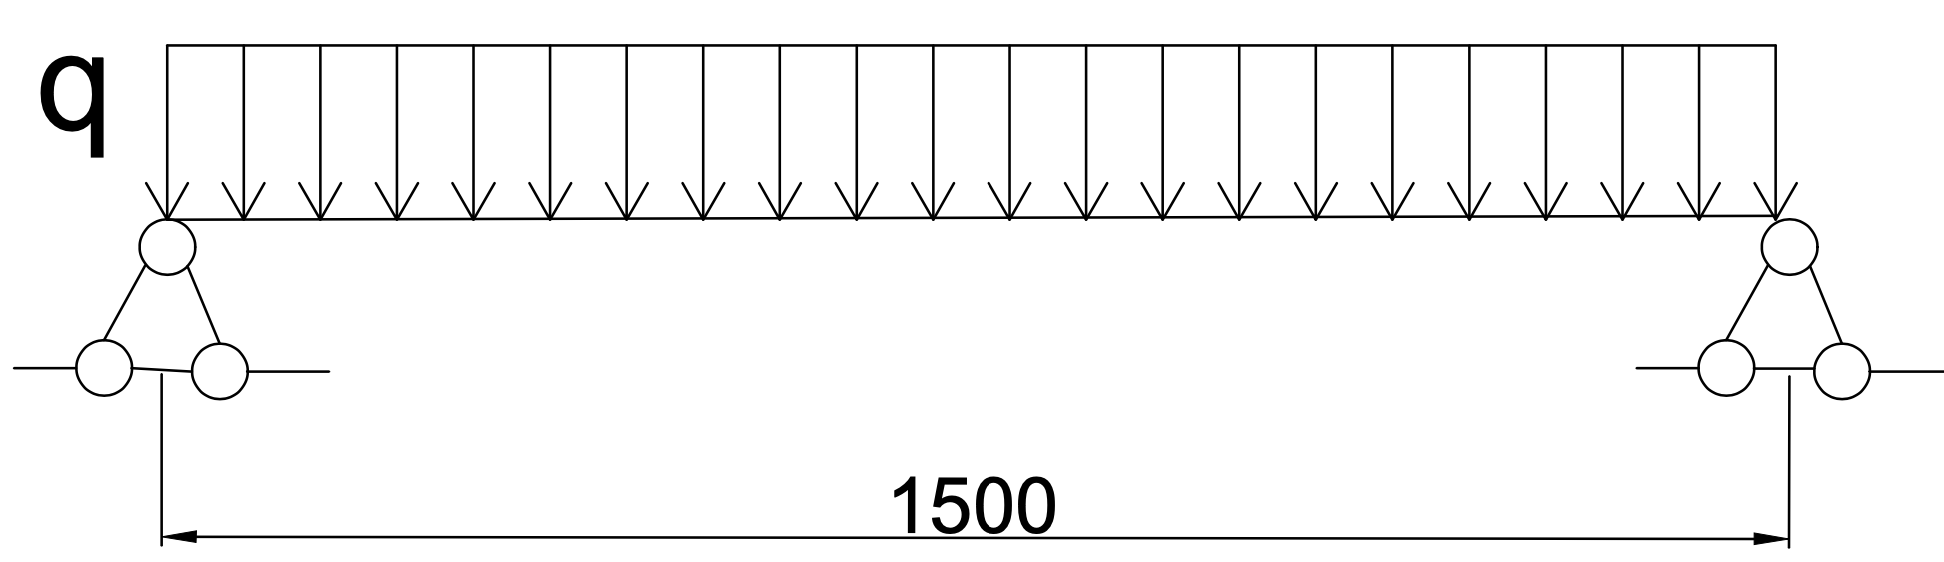
\includegraphics[width=0.8\linewidth]{figure/c4f1.png}
        \caption{小横杆受力简图}
        \label{fig:c4f1}
    \end{figure}

\quan{1} 均布荷载计算\\

小横杆的自重标准值:

$$p_1=0.0397 \times 1=0.0397 kN/m$$

脚手板的自重标准值:

$$p_2=\frac{0.35 \times 1.5}{2+1}=0.175 kN/m$$

施工荷载自重标准值:

$$Q=\frac{3 \times 1.5}{2+1}=1.5 kN/m$$

恒荷载做控制荷载设计值:

$$q_1=1.35\times(0.0397+0.175)+1.4\times 0.7\times 1.5=1.759 kN/m$$

活荷载做控制荷载设计值:

$$q_2=1.2\times(0.0397+0.175)+1.4\times 1.5=2.396 kN/m$$

\quan{2} 强度验算\\

恒荷载、活荷载二者取最大值,得出由活荷载做控制 $q=2.396 $kN/m。由于小横杆按照简支梁计算,故跨中弯矩值最大;

\begin{align}
    M_{max}=\frac{ql^2}{8}=\frac{2.396\times 1.05^2}{8}=0.33 kN\cdot m
\end{align}

式中:$q$ 为小横杆荷载设计值;$l$ 为小横杆计算跨度,即立杆横距。

计算最大应力,其中 $M_{max}$ 为最大弯矩, $W$ 为截面模量,取 $5.26 cm^3$,可得:

\begin{align}
    \label{fx:load}
    \sigma =\frac{M}{W}=\frac{0.33\times 10^6}{5.26\times10^3}=173.58N/mm^2
\end{align}

小横杆的计算强度 $173.58N/mm^2$ 小于小横杆的抗弯强度设计值 $205N/mm^2$,故强度满足要求!\\

\quan{3} 挠度验算\\

水平杆的挠度验算应满足 $v\leq [v] $,其中 $v$ 是挠度;小横杆的挠度计算式为:

\begin{align}
    V=\frac{5ql^4}{384EI}=\frac{5\times (0.397+0.175)\times 1050\times 10^4}{384\times 20.6\times 10^5\times 121870}=0.36 \text{mm}
\end{align}

式中 $E$ 为弹性模量,取$2.06\times 10^5$,$I$ 为惯性矩。

小横杆的最大挠度 0.36mm 小于 $1050.0/150=7.000$ 与 10mm,故挠度满足要求! \\

(2) 大横杆计算\\

按照《扣件式钢管脚手架安全技术规范》规定,大横杆按
照三跨连续梁进行强度和挠度计算,小横杆在大横杆的上面。
大横杆最大弯矩考虑均布荷载与集中荷载的最不利组合,且集中荷载、均布荷载最大弯矩值均出现在支座处,均上侧受拉。\\

\begin{figure}[thbp!]
    \centering
    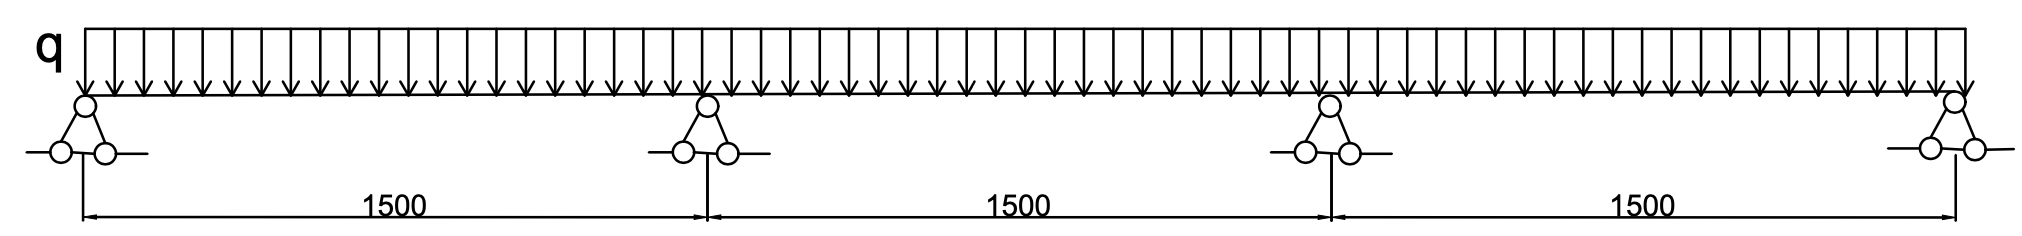
\includegraphics[width=1.0\linewidth]{figure/c4f2.png}
    \caption{大横杆受力简图}
    \label{fig:c4f2}
\end{figure}


\quan{1} 均布荷载值计算\\

小横杆的自重标准值:

$$p_1=0.0397 \times 1.05=0.042 kN/m$$

脚手板的自重标准值:

$$p_2=\frac{0.35 \times 1.5\times 1.05}{2+1}=0.184 kN/m$$

施工荷载自重标准值:

$$Q=\frac{3 \times 1.5\times 1.05}{2+1}=1.575 kN/m$$

恒荷载做控制荷载设计值:

$$q_1=\frac{[1.35\times(0.042+0.184)+1.4\times 0.7\times 1.575]}{2}=0.96 kN/M$$

活荷载做控制荷载设计值:

$$q_2=\frac{[1.2\times(0.042+0.184)+1.4\times 1.575]}{2}=1.27 kN/M$$

\quan{2} 强度验算\\

恒荷载、活荷载二者取最大值,得出由活荷载做控制 $q=1.27 kN/M$ 。由于大横杆最大弯矩考虑均布荷载与集中荷载的最不利组合,
且集中荷载、均布荷载最大弯矩值均出现在支座处,则

\begin{align}
    M_{max}=0.1pl^2+0.289ql
\end{align}

根据公式 \ref{fx:load} 可得 $\sigma =(0.503\times 10^6)/(5.26\times 10^3)=95.63 N/mm^2 \leq f=205 N/mm^2$\\
故强度满足要求!\\

\quan{3} 挠度验算\\

大横杆最大挠度考虑均布荷载与集中荷载的最不利组合;故荷载的最大挠度为:

\begin{align}
    V_{max}=\frac{0.99pl^4+2.76ql^3}{100EI}
\end{align}

带入数值得

$$V_{max}=\frac{0.99\times 0.397\times 1500^4+2.76\times (0.042+0.184)\times 1500^3/2}{100\times 2.06\times 10^5\times 121870}=0.792$$

大横杆的最大挠度 $0.792mm$ 小于 $1050.0/150=7.000$ 与 $10mm$,故挠度满足要求! \\

(3) 扣件抗滑计算\\

按照规范,直角,旋转单扣件承载力设计值取 $8.00kN$,纵向或横向水平杆与立杆连接时,扣件的抗滑承载力按照 《建筑施工扣件式钢管脚手架安全技术规范》 计算:

\begin{align}
    \label{fx:rc}
    R \leq R_c
\end{align}

竖向作用力设计值 $R$ 计算:

\quan{1} 大横杆自重标准值:$P_1=0.0397×1.5=0.059kN$

\quan{2} 小横杆自重标准值平均分配到两侧立杆:$P_2=0.0397×1.05/2=0.02kN$ 

\quan{3} 脚手板自重标准值平均分配到两侧立杆:$P_3=0.35×1.05×1.5/2=0.27kN$ 

\quan{4} 活荷载自重标准值平均分配到两侧立杆:$Q=3×1.05×1.5/2=2.36kN$

根据公式 \ref{fx:rc} ,荷载设计值:

$$R=1.2×(0.059+0.02+0.27)+1.4×2.36=3.72kN<R_c=8.0kN$$

故单扣件抗滑移能力可以满足要求。\\

(4 )立杆稳定性验算\\

根据 《建筑施工扣件式钢管脚手架安全技术规范》 ,立杆的稳定性应按照下列公式计算:

不组合风荷载时:

\begin{align}
    \label{fx:nw}
    \frac{N}{\varphi A}\leq f
\end{align}

组合风荷载时:

\begin{align}
    \label{fx:w}
    \frac{N}{\varphi A}+ \frac{M_W}{W}\leq f
\end{align}

式中:

$N$ 为计算立杆的轴向设计值;

$\phi$ 为轴心受压构件的稳定系数,根据规范取值;

$\lambda$ 为长细比,$\lambda =l_0/I$;

$l_0$ 为计算长度,根据规范计算;

$i$ 为截面回转半径,根据规范取值;

$A$ 为立竿截面面积,根据规范取值;

$M_W$ 为计算立杆段由风荷载设计值产生的弯矩,根据规范计算;

$f$ 为钢材的抗压强度设计值,根据规范取值;

按照组合风荷载计算,立杆的轴向设计值应该为:

\begin{align}
    \label{fx:Nzhou}
    N=1.2(N_{G1k+G2k})+0.9\times 1.4\sum N_{Qk}
\end{align}

式中:

$N_{G1k}$ 为脚手架结构自重产生的轴向力标准值; 

$N_{G2k}$ 为构配件自重产生的轴向力标准值;

$\sum N_{Qk}$ 为施工荷载产生的轴向力标准值总和,内、外立杆割按一纵距内施工荷载
总和的 $1/2$ 取值。

可得:

$N_{G1k}=18.0\times 0.144=2.59 kN$

$N_{G2k}=0.5\times (1.05+0.15)\times 1.5\times 2\times 0.35+1.5\times 2\times 0.16+1.5\times 18\times 0.01=1.41 kN$

$N=1.2\times (2.59+1.41)+0.85\times 1.4\times 4.5=10.15 kN$

立杆段由风荷载设计值产生的弯矩为:

\begin{align}
    M_W=0.9\times 1.4M_{Wk}=0.9\times 1.4\omega _kl_ah^2/10=0.21kN\cdot m
\end{align}

可得立杆稳定性的设计值为

$$\frac{10150}{0.265×5.06×10^2}+\frac{210000}{5.26×10^3}=115.6 N\cdot mm \leq f=205 N\cdot mm$$

故立杆的稳定性满足要求。\\

(5) 连墙件计算\\

连墙件杆件的强度应满足:

\begin{align}
    \sigma =\frac{N_l}{A_c}\leq 0.85f
\end{align}

稳定性应满足:

\begin{align}
    \label{fx:stb}    
    \frac{N_l}{\phi A}\leq 0.85f
\end{align}

\begin{align}
    N_l=N_{lw}+N_0
\end{align}

式中:

$A_c$ 为连墙件的净截面面积;  

$N_l$ 为连墙件轴向力设计值;   

$N_{lw}$ 为风荷载产生的连墙件轴向力设计值,按照公式 $N_{lw}=1.4\cdot w_k\cdot A_w$ 计算;

$N_0$ 为连墙件约束脚手架平面外变形所产生的轴向力,双排架取 $3.0kN$。

计算连墙件强度: 

$$\sigma=\frac{1.4×0.5×6×1.5×1.5+3}{506}=24.6 N/mm^2<0.85f=174 N/mm^2$$

故强度满足设计要求。

计算连墙件稳定性:

构件长细比为 $\lambda =l_0/I=150/1.59=9.43$,查表可得 $\phi=0.976$

根据公式 \ref{fx:stb} ,代入数据:

$$\sigma =\frac{12450}{0.976\times 1912}=6.67 N/mm^2<0.85f=174 N/mm^2$$

故稳定性满足设计要求。\\

(6) 地基承载力计算\\

立杆基础底面平均压力应满足下式:

\begin{align}
    p_k=\frac{N_k}{A} \leq f_g
\end{align}

\begin{align}
    f_c=k_c\times f_{g}
\end{align}

式中:

$p_k$ 为立杆基础底面处的平均压力标准值;   

$N_k$ 为上部结构传至立杆基础顶面的轴向力标准值; 

$A$ 为基础地面面积;                       

$f_g$ 为地基承载力特征值(kPa);$k_c$ 取 0.4。

可得 $N_{G1k}=H\times G_k=18.0\times 0.1444=2.59kN$、$N_{G2k}=1.41kN$、$N_{Qk}=4.54kN$;
按照公式 \ref{fx:Nzhou} 可得

$N=1.2\times (2.59+1.41)+1.4\times 4.54=9.9kN $

$Pk=9.9/(0.5×0.5)=39.6kN/m^2\leq f_g/0.4=99.4kN/m^2$

故地基承载力满足设计要求。\\

(7)最大允许搭设高度计算\\

双排脚手架的可搭设高度 $[H]$ 应按照下列公式计算,并取最小值:

不组合风荷载时:

\begin{align}
    \label{fx:bzh} 
    [H]=\frac{\phi Af-(1.2N_{G2k}+1.4\sum N_{Qk})}{1.2g_k}
\end{align}

组合风荷载时:

\begin{align}
    \label{fx:zh} 
    [H]=\frac{\phi Af-[1.2N_{G2k}+0.9\times 1.4(\sum N_{Qk}+\frac{M_{wk}}{W}\phi A)]}{1.2g_k}
\end{align}

式中:

$[H]$ 为脚手架最大允许搭设高度;

$g_k$ 为立杆承受的每米结构自重标准值,查规范可得 $g_k=0.1444kN/m$;

$A$ 为脚手架钢管截面面积; 

$f$ 为钢材强度设计值; 

$W$ 为截面模量。\\

当不组合风荷载时,将数据带入公式 \ref{fx:bzh} 得:

\begin{align*}
    [H] &=\frac{0.265\times 5.06\times10^{-4}\times 2.05\times 10^5-(1.2\times 1.41+1.4\times 4.5)}{1.2\times 0.1444}\\
    &=109.1m
\end{align*}

当组合风荷载时,将数据带入公式 \ref{fx:zh} 得:

\begin{align*}
[H] &=\frac{0.265\times 5.06\times10^{-4}\times 2.05\times10^5-[1.2\times 1.41+0.9\times 1.4\times(6.18+\frac{0.22\times 0.265\times 5.06\times 10^{-4}}{5.26\times 10^{-6}})]}{1.2\times 0.1444}\\
&=85m
\end{align*}

取最大允许搭设高度 50m,18.0m 符合要求。

\subsection{脚手架质量验收}

(1) 脚手架搭设前,对进入现场的各种构配件应按下列规定进行检查验收,不合格的应及时清除出场;
构配件应有相应的产品标识及产品质量合格证;构配件应有相应的技术参数及产品使用说明书;当对构配件质量有疑问时,应进行质量抽检和实
验。

(2) 脚手架在悬挑层顶梁板浇筑后及脚手架搭设前;作业层上施加荷载前;每搭设完两层后;达到设计高度后;遇有六级强风及以上风或大雨后;停
用超过一个月时应该进行检查与验收,按规定对脚手架工程的质量进行检查,合格后方可交付使用;

(3) 架子搭设和组装完毕,使用前必须由项目经理、技术负责人、项目安全负责人、架子班长等人员组成验收小组,
进行验收,并填写验收单。

(4) 脚手架使用期间必须设专人经常检查,符合要求后,必须经过项目经理签字批准,才能使用;
不合格部位必须及时修复或更换,符合规定后,方准许继续使用。 

\subsection{安全技术措施}
\subsubsection{脚手架搭设安全技术措施}

(1) 钢管架应设置避雷针,分置于主楼外架转角立杆之上,并联通大横杆,形成避雷网络。

(2) 脚手架不得搭设在距离外电架空线路的安全距离内,并做好可靠的安全接地处理。

(3) 定期检查脚手架,发现问题和隐患,在施工作业前应及时维修加固。

(4) 脚手架严禁钢木混用。

(5) 严禁脚手板存在探头板,铺设脚手板以及多层作业时,应尽量使施工荷载内、外传递平衡。

(6) 结构外脚手架每支搭一层,支搭完毕后,经项目部安全员验收合格后方可使用。任何班组长和个人,未经同意不得任意拆除脚手架部件。

(7) 脚手板不得集中堆料施荷,施工荷载不得大于 $4kN/m^2$。

\subsubsection{脚手架拆除安全技术措施}

(1) 拆除前应全面检查脚手架,根据检查结果指定施工计划,并报请批准;

(2) 拆架时应划分作业区,周围设置围栏竖立警示标志,地面应有专人指挥并禁止非作业人员进入;

(3) 拆架程序应先上后下,先搭后拆。即先插拉杆、脚手板、剪刀撑、斜撑;后拆小横杆、大横杆、立杆等,并按照一步一清的原则严格执行,禁止上下同时拆架;

(4) 连墙件应随拆除进度逐层拆除,拆除时应用临时支撑固定,然后才能拆除;

(5) 作业时应统一指挥,上下呼应,动作协调。当解开与人有关的结扣时,应先通知对方,以防坠落;

(6) 拆架时严禁触碰脚手架附近的电源线,以防触电;

(7) 拆架过程中不得中途换人,如必须换人必须将拆除情况交代清楚;

(8) 拆下的材料严禁抛掷,运至地面后应分类堆放,当天拆下的材料应及时运走;

(9) 高层建筑脚手架拆除时应配备良好的通讯设备;

(10) 强风、暴雨、暴雪等恶劣条件下禁止拆架,夜间不得进行拆架作业。
\section{模板工程专项安全施工方案}
\subsection{编制依据}

(1) 《建筑工程施工质量验收统一标准》(GB50300-2001)

(2) 《建筑结构荷载规范》(GB50009-2001)

(3) 《建筑施工模板安全技术规范》(JGJ162-2008)

(4) 《建筑施工扣件式钢管脚手架安全技术规范》(JGJ130-2011)

(5) 《建筑施工脚手架安全技术统一标准》(GB51210-2016)

(6) 《建筑施工安全检查标准》(JGJ59-2011)

(7) 《混凝土结构工程施工及验收规范》(GB50204-2015) 

\subsection{模板支撑架搭设要求}

(1) 必须设置纵横扫地杆。纵向扫地杆应采用直角扣件固定在距底座上皮不大于200mm 处的立杆上,
横向扫地杆也应采用直角扣件固定在紧靠纵向扫地杆下方的立杆上。当立杆基础不在同一高度上时,必须将高出的纵向扫地杆向低处延长两跨与立杆固定,高低差不应大于 1m。

(2) 立杆应采用对接接头,且接头位置不应设置在同一步内,同一步立杆的两个相隔接头在高度方向错开的距离不宜小于 500,
各接头中心至柱节点的距离不宜大于步距的 1/3。

(3) 纵向水平杆接长宜采用对接扣件连接,对接扣件应交错布置,两根相邻纵向水平杆接头不宜设置在同步或同跨内,
不同步或不同跨两个相邻接头在水平方向错开的距离不应小于 500m,各接头中心至最近主节点的距离不宜大于纵距的 1/3。

(4) 搭接长度不应小于 1m,应等距离设置 3 个旋转扣件固定,端部扣件盖板边缘至搭接纵向水平杆端的距离不应小于 100mm。

\subsection{模板计算书}
\subsubsection{基本参数}

(1) 钢筋混凝土板厚 $120mm$,板的模板采用木胶合板厚 $15mm$,面板下次愣采用 $40\times 80mm$ 木方,间距 $300mm$,主楞采用 $60\times 100mm$ ,木方间距 $500mm$,支撑体系采用 $\phi 48.3\times 3.6mm$ 钢管。

(2) 梁尺寸 $300\times 700mm$,模板采用木胶合板厚 $18mm$,侧模次楞采用 $40\times 80mm$ 木方, 布置间距 $200mm$,采用 $M20$ 对拉螺栓加固,
间距为 $250mm$,梁底次楞采用 $40\times 80mm$ 木方,次楞间距 $150mm$,梁模板主楞采用 $40\times 80mm$ 木方,间距 $500mm$,支撑体系采用 $Φ48.3\times 3.6mm$ 钢管。

(3) 柱尺寸 $500\times 500mm$ ,计算高度取 $9.0m$,模板采用木胶合板厚 $18mm$,次楞采用 $40\times 80mm$ 木方,间距为 $115mm$,
柱箍间距 $400mm$,最下一层柱箍距柱根间距为 $200mm$,最上一层柱箍距柱顶间距为 $200mm$,柱箍螺栓采用 $M18$。

\subsubsection{模板安全性验算}

(1) 对板的安全性验算\\

\quan{1} 楼板验算\\

根据《建筑结构荷载规范》(GB50009-2012),查得相关构件的标准荷载值如下:

模板自重标准值取 $G_{1k}=0.5 kN/m^2$

混凝土自重标准值取 $G_{2k}=24\times 0.12=2.88 kN/m^2 $

钢筋自重标准值取 $G_{3k}=1.1\times 0.12=0.132 kN/m^2$

施工活荷载标准值取 $2.5kN$($2.5kN/m$)

当活荷载作为均布线性荷载控制时:

\[q_1=0.9\times 1.0\times [1.2(500+2880+132)+1.4\times 2500]=6942 N/m\]

当恒荷载作为均布线性荷载控制时:

\[q_1=0.9\times 1.0\times [1.35(500+2880+132)+0.7\times 1.4\times 2500]=6471 N/m\]

$q$ 取较大值,故 $q=6942 N/m$

当作为集中荷载控制时:

\begin{align*}
    q_2&=0.9\times 1.0\times 1.2\times (500+2880+132)=3792 N/m\\
    P&=0.9\times 1.0\times 1.4\times 2500=3150N
\end{align*}

施工荷载为均布线荷载时的弯矩值为:

\begin{align}
    \label{fx:5.0}
    M_1=0.1ql^2=0.1\times 6.942\times 0.32=0.06kN\cdot m
\end{align}

施工荷载为集中荷载时的弯矩值为:

\begin{align}
    M_2&=0.1ql^2+0.213pl\\
    &=0.1\times 3.79\times 0.32+0.213\times 3.15\times 0.3 \notag\\
    &=0.23 kN \cdot m \notag
\end{align}

弯矩取最大值计算,故 $M=0.23kN\cdot m$\\

对板做强度验算,按照三跨连续梁计算,

\begin{align}
    \label{fx:5.1}
    \sigma =\frac{M}{W}
\end{align}

式中,$M$ 为模板受到最大弯矩值;$W$ 为截面模量,矩形的截面模量公式为:

\begin{align}
    \label{fx:5.2}
    W=bh^2/6
\end{align}

式中,$b$ 为模板计算宽度;$h$ 为模板厚度。代入数据可得:

\begin{align*}
    W&=1000\times 152/6=37500 mm^3\\
    \sigma &=230000/37500=6.1 N/mm2<f=22 N/mm^2
\end{align*}

故板的强度满足要求。\\

对板做挠度验算,按照三跨连续梁计算,

\[q=0.9\times 1.0\times (500+2880+132)=3002 N/m\]

\begin{align}
    \label{fx:5.3}
    V_{max}=\frac{0.990ql^4}{100EI}
\end{align}

$E$ 为模板的弹性模量,取 $E=10000 N/mm^2$;$I$ 为截面惯性矩,计算公式为:

\begin{align}
    \label{fx:5.4}
    I=\frac{bh^3}{12}
\end{align}

代入数据得 $I=1000\times 15^3/12=281250 mm^4$。将截面惯性矩代入公式 \ref{fx:5.3} 得

\begin{align*}
    V&=\frac{0.99\times (3.002\times 10^2\times 300\times 10^2)}{100\times 10000\times 281250}\\
    &=0.058 mm < [v]=1/400=0.75 mm
\end{align*}

故板的挠度满足要求。\\

\quan{2} 板的次楞验算\\

板次楞采用 40×80mm 木方,间距 300mm,主楞间距 500mm。次楞的荷载按三跨连续梁计算受力,对板的次楞做强度验算:

\begin{align*}
    q_1&=0.9\times [1.2(500+2880+132)+1.4\times 2500]\times 0.3=1972 N/m \\
    q_2&=0.9\times (500+2880+132)\times 0.3=1.00 N/m
\end{align*}

分别按照公式 \ref{fx:5.0}、\ref{fx:5.2} 计算得出最大弯矩值与截面模量:

\begin{align*}
    M&=0.1\times 1.972\times 0.5^2=0.047 kN \cdot m\\
    W&=40\times 80^2 /6=42667 mm^2
\end{align*}

随后按照公式 \ref{fx:5.1} 求出板的次楞的强度:

\[
    \sigma = \frac{47000}{42667}=1.112 N/mm^2< f=17N/mm^2
\]

故次楞的强度满足要求。\\

对板的次楞做挠度验算,根据公式 \ref{fx:5.4} 算出次楞的最大截面惯性矩 $I$

\[
    I=40\times 80^3 /12=1706667 mm^4
\]

再将结果代回公式 \ref{fx:5.3},便可求出次楞的挠度设计值:

\begin{align*}
    V&=\frac{0.99\times 1 \times 500^4}{100\times 10000\times 1706667}\\
    &=0.0204 mm<[v]=1/400=1.25mm
\end{align*}

故次楞的挠度也满足要求。\\

\quan{3} 板的主楞验算\\

主楞采用 $60\times 100mm$ 木方,间距 $500mm$,板支撑在主楞上间距 $900mm$。由于木楞自重较小,因此计算时将其忽略
,主楞按照三跨梁计算,对主楞做强度验算:

\begin{align*}
    q_1&=0.9\times [1.2(500+2880+132)+1.4\times 2500]\times 0.5=3781 N/m \\
    q_2&=0.9\times (500+2880+132)\times 0.5=1.58 N/m
\end{align*}

按照主楞的最大弯矩公式求出主楞的最大弯矩值:

\begin{align}
    M=0.289q_1l=0.289\times 3.78\times 0.9=0.98 kN \cdot m
\end{align}

按照公式\ref{fx:5.2} 计算得出主楞的截面模量:

\[
    W=60\times 100^2 /6=100000 mm^2
\]

随后按照公式 \ref{fx:5.1} 求出板的主楞的强度:

\[
    \sigma = \frac{980000}{100000}=9.8 N/mm^2< f=17N/mm^2
\]

故主楞的强度满足要求。\\

对板的主楞做挠度验算,根据公式 \ref{fx:5.4} 算出次楞的最大截面惯性矩 $I$

\[
    I=60\times 100^3 /12=5000000 mm^4
\]

再将结果代回公式 \ref{fx:5.3},便可求出次楞的挠度设计值:

\begin{align*}
    V&=\frac{0.99\times 1580 \times 900^3}{100\times 10000\times 5000000}\\
    &=0.23 mm<[v]=1/400=2.25mm
\end{align*}

故主楞的挠度也满足要求。\\

\quan{4} 板的立杆验算\\

楼板支模高度 $9.0m$,属于高支模,立杆采用 $\phi 48.3\times 3.6$ 钢管,底部设置一道拉结杆,向上每 $1.5m$ 设置一道拉结杆。

查规范可得各个关键部件的自重标准值:

支撑自重为 $0.1444\times 9.0=1.29kN$

混凝土自重为 $24\times 0.12\times 0.5\times 0.9=1.29kN $

钢筋自重为 $1.1\times 0.12\times 0.5\times 0.9=0.05kN$

按照各个部件的自重标准值,能够求出恒荷载与活荷载的值:

恒荷载为 $1.27+1.29+0.05=2.63kN$

活荷载为 $2.5\times 0.5\times 0.9=1.125kN$

当活荷载控制时:

\[N_1=0.9\times (1.2\times 2.63+1.4\times 1.125)=4.25kN\]

当恒荷载控制时:

\[N_2=0.9\times (1.35\times 2.63+1.4\times 0.7\times 1.125=4.18kN\]

立杆轴向力取值取最大荷载值,即 $N=4.25 kN$

计算满堂脚手架的立杆长度的公式如下:

\begin{align}
\label{fx:5.5}
l_0&=k\mu_1(h+2a)\\
\label{fx:5.6}
l_0&=k\mu_2h
\end{align}

式中:
$k$ 为满堂支撑架立杆计算长度附加系数,取 1.185;   

$h$ 为步距 1.5m;                           

$a$ 为立杆伸出顶层水平杆中心线至支撑点长度 20mm;

$\mu_1$、$\mu_2$ 为满堂支撑架整体稳定因素的单杆计算长度系数,
根据《建筑施工扣件式脚手架安全技术规范》取值为 $\mu_1=1.54$、$\mu_2=1.951$

将上述数据代入公式 \ref{fx:5.5}、\ref{fx:5.6} 得:

\begin{align*}
    l_1&=1.185\times 1.54\times (1.5+2\times 0.2)=3.467 m\\
    l_2&=1.185\times 1.951\times 1.5=3.468 m
\end{align*}

$l_0$ 取二者最大值,即 $l_0=3.468 m$,随后根据公式 $\lambda=l_0/i$ 求出长细比为

\[
    \lambda = \frac{3.468}{1.59}=218
\]

查表可得轴心受压构件的稳定系数 $\phi =0.153$,再将上述所有数据代入下式可得出杆的弯曲正应力 $\sigma $

\begin{align}
\sigma &=\frac{N}{\phi A}\\
&=\frac{4180}{0.153\times 506} \notag\\
&=53.9 N/mm^2<f=205 N/mm^2 \notag
\end{align}

故主杆满足设计要求。\\

(2) 对梁的安全性验算\\

\quan{1} 梁模板计算\\

梁模板计算取首层截面尺寸最大的梁进行计算,截面尺寸为 300×700mm,模板采用 18mm
厚木模板,次楞间距 200mm。

新浇混凝土作用于模板的侧压力,可以使用下列公式做计算:

\begin{align}
    \label{fx:5.7}
    F&=0.22\gamma_c t_0\beta_1 \beta_2V^{\frac{1}{2}}\\
    \label{fx:5.7a}
    F&=\gamma_c H
\end{align}

式中:

$\gamma_c$ 为混凝土重力密度,根据规范取值 $24 kN/m^3$;

$t_0$ 为混凝土入模温度,根据

\begin{align}
\label{fx:5.8}
t_0=\frac{200}{t+15}
\end{align}

可以计算出,$t$ 为当前温度;为方便计算,$t$ 取 20 摄氏度;

$\beta_1$ 为外加剂影响修正系数,根据规范取 1.0;

$\beta_2$ 为混凝土坍落度影响修正系数,根据规范取 1.0;

$V$ 为混凝土浇筑速度,根据计算手册,为方便取 $2 m/h$;

$H$ 混凝土侧压力计算位置至新浇筑混凝土顶面总高度为 700mm;

根据公式 \ref{fx:5.8} 、\ref{fx:5.7} 和 \ref{fx:5.7a} 分别可得 

    \begin{align*}
        t_0&=200/(20+15)=5.71\\
        F_1&=0.22\times 24\times 5.71\times 1\times 1\times 2^{\frac{1}{2}}=42.6 kN/m^2\\
        F_2&=24\times 0.7=16.8 kN/m^2
    \end{align*}

则新浇混凝土作用于模板的侧压力的标准值 $G_{4k}=16.8 kN/m^2$,查表得可变荷载标准值 $Q_{2k}=4 kN/m^2$,所以

当恒荷载做控制时

\[
    q_1=0.9\times 0.7\times (1.35\times 16.8+1.4\times 0.7\times 4)=15.5 kN/m
\]

当活荷载做控制时

\[
    q_1^{'}=0.9\times 0.7\times (1.2\times 16.8+1.4\times 4)=14.4 kN/m
\]

荷载组合强度取最大值 $15.5 kN/m$,荷载组合的挠度计算值为

\[
    q=0.9\times 0.7\times 16.8=10.05 kN/m
\]

对梁模板做强度验算,分别根据公式 \ref{fx:5.0}、\ref{fx:5.2} 计算得出最大弯矩值与截面模量:

\begin{align*}
    M&=0.1\times 15.5\times 200^2=620000 N \cdot mm\\
    W&=1000\times 18^2 /6=54000 mm^2
\end{align*}

随后按照公式 \ref{fx:5.1} 求出板的次楞的强度:

\[
    \sigma = \frac{62000}{54000}=1.1 N/mm^2< f=17N/mm^2
\]

故梁模板的强度满足要求。\\

对梁模板做挠度验算,根据公式 \ref{fx:5.4} 算出次楞的最大截面惯性矩 $I$

\[
    I=1000\times 18^3 /12=486000 mm^4
\]

再将结果代回公式 \ref{fx:5.3},便可求出次楞的挠度设计值:

\begin{align*}
    V&=\frac{0.99\times 10.05 \times 200^3}{100\times 10000\times 486000}\\
    &=0.3 mm<[v]=1/400=0.5mm
\end{align*}

故梁模板的挠度也满足要求。\\

\quan{2} 梁侧模次楞验算\\

梁侧次楞采用 40×80mm 木方,间距 200mm,主楞间距 500mm。木楞自重影响较小,计算时忽略不计,次楞的荷载按三跨连续梁计算受力,对板的次楞做强度验算:

\begin{align*}
    q_1&=0.9\times 0.2\times [1.35\times 1.68+1.4\times0.7\times 2]=4.43 kN/m \\
    q_2&=0.9\times 16.8\times 0.2=3.02 kN/m
\end{align*}

分别按照公式 \ref{fx:5.0}、\ref{fx:5.2} 计算得出最大弯矩值与截面模量:

\begin{align*}
    M&=0.1\times 4430\times 500^2=110000 N \cdot mm\\
    W&=40\times 80^2 /6=42667 mm^2
\end{align*}

随后按照公式 \ref{fx:5.1} 求出板的次楞的强度:

\[
    \sigma = \frac{110000}{42667}=2.6 N/mm^2< f=17N/mm^2
\]

故梁侧模次楞的强度满足要求。\\

对梁侧模的次楞做挠度验算,根据公式 \ref{fx:5.4} 算出次楞的最大截面惯性矩 $I$

\[
    I=40\times 80^3 /12=1706667 mm^4
\]

再将结果代回公式 \ref{fx:5.3},便可求出次楞的挠度设计值:

\begin{align*}
    V&=\frac{0.99\times 3.02 \times 500^4}{100\times 10000\times 1706667}\\
    &=0.264 mm<[v]=1/400=1.25mm
\end{align*}

故梁侧模的次楞的挠度也满足要求。\\

\quan{3} 侧模对拉螺栓验算\\

对拉螺栓采用 M12,水平间距 500mm,竖向间距 200mm,对拉螺栓最大轴力设计值可按以下公式求出:

\begin{align}
    \label{fx:5.9}
    N^b_t>N&=abF_s
\end{align}

式中 $a$、$b$ 分别为对拉螺栓的水平间距和竖向间距, $F_s$ 为新浇混凝土作用于模板上的侧压力、振捣混凝土对垂直模板产生的水平荷载或倾倒混凝土时作用于模板上的侧压力设计值:

\begin{align}
    \label{fx:5.9a}
    F_s=0.95(r_GF+r_QQ_{3k})
\end{align}

或者

\begin{align}
    \label{fx:5.9b}
    F_s=0.95(r_GG_{4k}+r_QQ_{3k})
\end{align}

其中 0.95 为荷载值折减系数,针对本项目应该使用公式 \ref{fx:5.9b},代入数据得

\[
F_s=0.95\times(1.35\times 16.8+1.4\times 2.0)=24.21 kN/m^2    
\]

将计算得出的 $F_s$ 代回 \ref{fx:5.9},得

\[N=0.2\times 0.5\times 24.21=2.42 kN\]

查表得 M12 对拉螺栓的 $N_t^b$ 值为 $12.9 kN$,因为 $2.42<12.9$,故对拉螺栓的设计值可以满足要求。\\

\quan{4} 梁底模验算\\

取 300 宽板计算,梁底设置 3 个 40×80 次楞,间距 150mm,按照三跨连续板计算,根据《建筑结构荷载规范》(GB50009-2012),
查得相关构件的标准荷载值如下:

模板自重标准值取 $0.5 kN/m^2$

混凝土自重标准值取 $2.4\times 0.7=16.8 kn/m^2$

钢筋自重标准值取 $1.5\times 0.7=1.05 kN/m^2$

当由活荷载控制荷载时:

\[q_1=0.9\times 0.3\times[1.2\times(0.5+16.8+1.05)+1.4\times 2]=6.71 kN/m\]

当由恒荷载控制荷载时:

\[q_1^{'}=0.9\times 0.3\times[1.35\times(0.5+16.8+1.05)+1.4\times0.7\times 2]=7.2 kN/m\]

$q_1$ 取二者最大值,即 $7.2 kN/m$,$q_2=0.9\times 0.3\times (0.5+16.8+1.05)=4.9 kN/m$

对梁底模模板做强度验算,按照公式

\begin{align}
    \label{fx:5.X}
    M=0.096ql^2
\end{align}

可以计算得出截面的最大弯矩,按照公式\ref{fx:5.2} 可以计算得出截面模量:

\begin{align*}
    M&=0.096\times 7.2\times 150^2=15552 N \cdot mm\\
    W&=1000\times 18^2 /6=54000 mm^2
\end{align*}

随后按照公式 \ref{fx:5.1} 求出梁底模模板的强度:

\[
    \sigma = \frac{15552}{54000}=0.28 N/mm^2< f=17N/mm^2
\]

故梁底模模板的强度满足要求。\\

对梁侧模的次楞做挠度验算,根据公式 \ref{fx:5.4} 算出次楞的最大截面惯性矩 $I$

\[
    I=1000\times 18^3 /12=486000 mm^4
\]

再将结果代回公式 \ref{fx:5.3},便可求出梁底模模板的挠度设计值:

\begin{align*}
    V&=\frac{0.99\times 4.9 \times 150^4}{100\times 10000\times 486000}\\
    &=0.005 mm<[v]=1/400=0.3mm
\end{align*}

故梁底模模板的挠度也满足要求。\\

\quan{5} 梁底模次楞验算\\

梁底模次楞采用 40×80mm 木方,间距 150mm,主楞间距 500mm。木楞自重影响较小,计算时忽略不计,次楞的荷载按三跨连续梁计算受力,当荷载由活荷载控制时:

\[q_1=0.9\times 0.15\times [1.2\times (0.5+16.8+0.15)+1.4\times 2]=3.20 kN/m\]

当荷载由恒荷载控制时:

\[q_1=0.9\times 0.15\times [1.35\times (0.5+16.8+0.15)+1.4\times0.7\times 2]=3.44 kN/m\]

$q_1$ 取二者最大值,即 $3.44 kN/m$,$q_2=0.9\times 0.15\times (0.5+16.8+0.15)=2.3 kN/m$

分别按照公式 \ref{fx:5.0}、\ref{fx:5.2} 计算得出最大弯矩值与截面模量:

\begin{align*}
    M&=0.1\times 3440\times 500^2=86000 N \cdot mm\\
    W&=40\times 80^2 /6=42667 mm^2
\end{align*}

随后按照公式 \ref{fx:5.1} 求出梁底模次楞的强度:

\[
    \sigma = \frac{86000}{42667}=2.02 N/mm^2< f=17N/mm^2
\]

故梁底模次楞的强度满足要求。\\

对梁底模次楞做挠度验算,根据公式 \ref{fx:5.4} 算出梁底模次楞的最大截面惯性矩 $I$

\[
    I=40\times 80^3 /12=1706666 mm^4
\]

再将结果代回公式 \ref{fx:5.3},便可求出次楞的挠度设计值:

\begin{align*}
    V&=\frac{0.99\times 2.30 \times 500^4}{100\times 10000\times 1706666}\\
    &=0.05 mm<[v]=1/400=1.25mm
\end{align*}

故梁底模次楞的挠度也满足要求。\\

\quan{6} 梁底模主楞验算\\

梁底模主楞采用 40x80mm 木方,间距 500mm,支撑在主楞上间距 300mm,由于木楞的自重对结构的影响较小,故计算时忽略木楞自重,梁底主楞按照单跨简支梁计算,由活荷载做控制

\begin{align*}    P_1&=\frac{3550\times 0.3}{2}=0.53 kN\\
    P_2&=\frac{2300\times 0.3}{2}=0.34 kN
\end{align*}

对梁底模主楞做强度验算,按照公式

\begin{align}
    \label{fx:5.A}
    M=\frac{1}{4}p_1l
\end{align}

可以计算得出截面的最大弯矩,按照公式\ref{fx:5.2} 可以计算得出截面模量:

\begin{align*}
    M&=\frac{1}{4}\times 0.53\times 0.3=40000 N \cdot mm\\
    W&=40\times 80^2 /6=42666 mm^2
\end{align*}

随后按照公式 \ref{fx:5.1} 求出梁底模主楞的强度:

\[
    \sigma = \frac{40000}{42666}=1.0 N/mm^2< f=17N/mm^2
\]

故梁底模主楞的强度满足要求。\\

对梁底模主楞做挠度验算,根据公式 \ref{fx:5.4} 算出梁底模主楞的最大截面惯性矩 $I$

\[
    I=40\times 80^3 /12=1706666 mm^4
\]

再将结果代回简支梁最大挠度公式 

\begin{align}
    V_{max}&=\frac{5p_2l^3}{384EI}\\
    &=\frac{5\times 340\times 300^3}{384\times 10000\times 170666} \notag \\
    &=0.07mm<[v]=1/400=0.75mm \notag
\end{align}

便可求出梁底模主楞的挠度也满足要求。\\

(3) 对柱的安全性验算\\

\quan{1} 柱箍间距计算

柱选取首层截面尺寸最大的柱进行计算,截面尺寸为 500×500mm,计算高度 9.0m, 模板采用 18mm 厚木模板,竖楞采用 40×80mm 木方,间距 100mm,用柱箍固定,柱箍处用 M18 螺栓加固。

当柱模板为木面板时柱箍间距应按照如下公式计算:

\begin{align}
    \label{fx:5.B}
    L \leq 0.783\sqrt[3]{\frac{EI}{Fb}}
\end{align}

式中 $L$ 为柱箍间距,$E$ 为面板的弹性模量,取 10000,$b$ 为面板宽度,为 500mm,根据公式 \ref{fx:5.4} 可求出 $I$ ,
根据公式 \ref{fx:5.7} 可以求出式中的 $F$:

\begin{align*}
I&=\frac{500\times 18^3}{12}=243000\\
F&=0.22\times 24\times 5.71\times 1\times 1\times 2^{\frac{1}{2}}=42600 N/mm^2
\end{align*}

将上述所有数值代回公式 \ref{fx:5.B} 可得出柱箍间距 $L$ 为

\[L \leq 0.783\times \sqrt[3]{\frac{10000\times 243000}{4260000\times 10^{-6}\times 500}}=399mm\]

此外,柱箍间距还应满足

\begin{align}
    \label{fx:5.C}
    L \leq \sqrt{\frac{8Wf_m}{F_sb}}=\sqrt{\frac{8\times 27000\times 35}{42600\times 10^{-6}\times 500}}=595 mm
\end{align}

比较这两个结果,二者取最小值,即柱箍间距 $L=400mm$。

\quan{2} 柱模板安全验算

墙体模板受力可以简化为三跨梁连续梁,根据公式 \ref{fx:5.7} 和 \ref{fx:5.7a} 可以求出新教混凝土作用于模板上的侧压力设计值 $G_{4k}$

\begin{align*}
    F_1&=0.22\times 24\times 5.71\times 1\times 1\times 2^{\frac{1}{2}}=42600 N/mm^2\\
    F_2&=\times 9000=216 kN/m^2
\end{align*}

二者取较小值,则新教混凝土作用于模板上的侧压力设计值 $G_{4k}=42.6 kN/m^2$,按照规范取钢筋自重标准值 $G_{3k}=2kN/m^2$

当活荷载做控制时

\[q_1=0.9\times 0.5\times (1.2\times 42.6+1.4\times 2)=22.7kN \cdot m\]

当恒荷载做控制时

\[q_1^{'}=0.9\times 0.5\times (1.35\times 42.6+1.4\times 0.7\times 2)=26.7kN \cdot m\]

$q_1$ 取二者最大值,即 $26.7 kN/m$,$q_2=0.9\times 42.6=38.34 kN/m$

分别按照公式 \ref{fx:5.0}、\ref{fx:5.2} 计算得出最大弯矩值与截面模量:

\begin{align*}
    M&=0.1\times 26.7\times 100^2=26700 N \cdot mm\\
    W&=100\times 18^2 /6=54000 mm^2
\end{align*}

随后按照公式 \ref{fx:5.1} 求出柱模板的强度:

\[
    \sigma = \frac{54000}{26700}=2.02 N/mm^2< f=17N/mm^2
\]

故柱模板的强度满足要求。\\

对柱模板做挠度验算,根据公式 \ref{fx:5.4} 算出柱模板的最大截面惯性矩 $I$

\[
    I=500\times 18^3 /12=243000 mm^4
\]

再将结果代回公式 \ref{fx:5.3},便可求出柱模板的挠度设计值:

\begin{align*}
    V&=\frac{0.99\times 38.3 \times 100^4}{100\times 10000\times 486000}\\
    &=0.15 mm<[v]=1/400=1.25mm
\end{align*}

故柱模板的挠度也满足要求。\\

\quan{3} 柱竖楞验算

柱竖楞的荷载按三跨连续梁计算受力,

\begin{align*}
    q_1&=0.9\times 0.1\times(1.35\times 42.6+1.4\times 0.7\times 2)=5.4 kN/m\\
    q_2&=0.9\times 0.1\times 42.6=3.83 kN/m
\end{align*}

分别按照公式 \ref{fx:5.0}、\ref{fx:5.2} 计算得出最大弯矩值与截面模量:

\begin{align*}
    M&=0.1\times 5400\times 500^2=86000 N \cdot mm\\
    W&=40\times 80^2 /6=42667 mm^2
\end{align*}

随后按照公式 \ref{fx:5.1} 求出柱竖楞的强度:

\[
    \sigma = \frac{86000}{42667}=2.02 N/mm^2< f=17N/mm^2
\]

故柱竖楞的强度满足要求。\\

对柱竖楞做挠度验算,根据公式 \ref{fx:5.4} 算出柱竖楞的最大截面惯性矩 $I$

\[
    I=40\times 80^3 /12=1706666 mm^4
\]

再将结果代回公式 \ref{fx:5.3},便可求出柱竖楞的挠度设计值:

\begin{align*}
    V&=\frac{0.99\times 3.83 \times 400^4}{100\times 10000\times 1706666}\\
    &=0.56 mm<[v]=1/400=1.25mm
\end{align*}

故柱竖楞的挠度也满足要求。\\

\quan{4} 柱箍验算

柱箍采用 40x80mm 的木材质,按照简支梁计算,使用公式 \ref{fx:5.D} 求得柱箍强度:

\begin{align}
    \label{fx:5.D}
    \frac{N}{A_n}+\frac{M_x}{W_nx}\leq f \ \text{或} \ (f_m)
\end{align}

其中

\begin{align}
\label{fx:5.E}
N&=\frac{1}{2}ql_3\\
&=0.5\times 17040\times 05=4040 N \notag\\
\label{fx:5.F}
q&=F_sl_1\\
&=42600\times 0.4=17040 N/mm \notag\\
\label{fx:5.G}
M_x&=\frac{ql_2^2}{8}=\frac{F_sl_1L_2^2}{8}\\
&=\frac{17040\times (500+15\times 2)}{8}=598317 N \cdot mm \notag
\end{align}

在公式 \ref{fx:5.D} 中的柱箍截面面积 $A_n=40\times 80=3200 mm^2$;柱箍界面抵抗矩 $W_{nx}=80^2\times 40/6=42666 mm^3$
将上述数据代回公式 \ref{fx:5.D} 中得

\begin{align*}
    \frac{N}{A_n}+\frac{M_x}{W_nx}=\frac{4040}{3200}+\frac{598317}{42666}=15.28 N/mm^2
\end{align*}

查表得 $f_m=17N/mm^2$,$15.28<17N/mm^2$ 故强度满足要求。

对柱箍做挠度验算,$q_2=\times 0.9\times 42.6\times 0.4=15.3 N/mm^2$,
根据公式 \ref{fx:5.4} 算出柱箍的最大截面惯性矩 $I$

\[
    I=40\times 80^3 /12=1706666 mm^4
\]

再按照简支梁计算公式将结果代回

\begin{align*}
    V_{max}&=\frac{5q_2l^3}{384EI}\\
    &=\frac{5\times 15.3\times (500+15\times 2)^3}{384\times 10000\times 170666}\\
    &=0.92mm<[v]=1/400=1.225mm
\end{align*}

便可求出柱箍的挠度也满足要求。\\

\quan{5} 螺栓验算

螺栓采用 M18,竖向间距 400mm。根据公式 \ref{fx:5.9} 、\ref{fx:5.9b} 可得

\begin{align*}
    F_s&=0.95\times(1.2\times 42.6+1.4\times 2)=51.2 kN/m^2
    N&=0.5\times 0.3\times 51.2=7.68 kN
\end{align*}

查表得 M18 螺栓的 $N^b_t$ 值为 $29.6 kN>7.68 kN$,故螺栓满足设计要求。

\subsection{模板安装及拆除}
\subsubsection{模板安装}

(1) 模板安装前应该审查模板结构设计说明书,确保手续齐全

(2) 应进行全面的安全技术交底,操作班组应该熟悉设计与施工说明书,并做好模板安装作业的分工准备

(3) 模板安装应该按照设计与施工说明书按顺序拼装。木杆、钢管、门架等支架立柱不得混用

(4) 竖向模板和支架立柱支撑部分安装在基土之上时,应加设垫板,垫板应有足够的强度和支承面积,且应中心承载,基土应坚实,并附有排水措施

(5) 模板及其支架在安装过程中必须设立有效的防止倾覆的临时固定设施

(6) 现浇钢筋混凝土梁板当跨度大于 4 米时,模板应起拱。

(7) 模板应有足够的承载能力,刚度和稳定性。

(8) 楼板模板施工前应先弹线,根据弹线搭设脚手架,先搭设梁底然后搭设板底,调整梁底钢管标高,调平后,铺设梁底模,梁底模两侧用扣件锁紧,防止梁底模跑位; 

(9) 梁钢筋绑扎完毕后,封梁侧模,梁侧模应落在梁底模上,梁模板转角处必须设置木方; 

(10) 铺设主次龙骨,模板拼缝要严密,用对拉螺栓固定模板, 楼板模板压在梁侧模上。

\subsubsection{模板拆除}

(1) 模板拆除应该经过相关管理人员的批准,按照国家标准《混凝土结构工程施工质量验收规范》(GB50204)的有关规定执行;

(2) 当混凝土未达规定强度,或已经达到规定强度,但需提前拆模的,必须经过计算和主管部门的批准后方可拆除;

(3) 大体积混凝土的拆模时间除了要满足混凝土强度要求之外,还应使得混凝土内外温差降低到 25 摄氏度以下时方可拆模;

(4) 拆模前应确定所使用的工具有效可靠,扳手等工具必须挂在工具袋内;

(5) 拆模的顺序和方法应该按照模板的设计规定执行,当无设计要求时,应按照先支的后拆、后支的先拆、先拆非承重模板
后拆承重模板,并应从上至下进行拆除;

(6) 多人同时作业时,应分工明确,统一信号,应预留出足够的操作面,人员要站在安全处;

(7) 在拆除互相搭连并影响其他后拆模板的支撑时,应布设临时支撑。拆模时逐块拆卸,不得使用大锤和撬棍成片撬落或砸倒拉倒;

(8) 拆除有洞口的模板时,应采取防止操作人员坠落的措施,洞口模板拆除后,应按国家先行标准《建筑施工高处作业安全技术规范》(JGJ80)
的有关规定进行防护。

\subsection{模板工程安全措施}

(1) 模板施工属高空作业,作业人员必须佩戴安全帽,安全绳并设置妥当,经医生检查认为不适宜高空作业的人员,不得进行高空作业

(2) 工作前应检查使用的工具是否牢固可用,扳手等工具必须用绳系在身上,钉子必须放在工具袋内;

(3) 安装与拆除五米以上的模板时,应搭设脚手架并设置防护栏杆,严谨上下共同作业;

(4) 遇六级以上的大风时应停止高空作业,雨雪后应先清扫施工现场,等待场地不滑时在进行作业;

(5) 两人抬运模板时要互相配合,协同工作。传递模板和工具时应先用绳子系牢固后再升降,不得随意乱抛。钢模板装拆时上下应有人接应,钢模板及其配件应随装随拆随运;

(6) 不得在脚手架上堆放模板;

(7) 支撑不得搭设在门窗框和脚手架上,斜撑和拉杆应设置在 1.8m 以上

(8) 支模过程中如遇中途停止,应将支撑,搭头,柱头等固定妥善,拆模间歇时应将已活动的模板和支撑等运走或妥善堆放,防止踏空;

(9) 模板上的预留洞口,应在留设后盖好;混凝土板上的预留洞口应在模板拆除之后盖好。

\subsection{成品保护}

(1) 对违反模板安全操作规范的,有损害模板安全使用现象的行为应及时制止个纠正,多层板拆除后应及时清理并分规格摆放,码放的高度不得大于 1.5 米;

(2) 吊装物体时,应轻吊轻放,不准碰撞已施工模板;

(3) 不经相关人员同意,任何人不得私自拆模,拆除模板以不损坏墙体,表面及棱角为准;

(4) 安装和拆除模板时不得用大锤砸多层板,以免使多层板翘曲变形以及砸坏硂成品;

(5) 多层板运输和堆放时,应做好防水工作,堆放场地也要有排水措施。


\section{基坑支护结构专项施工方案}
\subsection{编制依据和工程概况}
\subsubsection{编制依据}

(1) 《建筑基坑支护技术规程》(JGJ120-2012)

(2) 《建筑桩基技术规范》(JGJ 94-2008)

(3) 《建筑基坑工程监测技术规范》(GB50497-2009)

(4) 《土层锚杆设计与施工规程》 (CECS22:90)

(5) 《深基坑工程施工安全技术规范》 JGJ311-2013

(6) 《混凝土结构设计规范》 GB50010-2015

(7) 《建筑结构静力计算手册》

\subsubsection{工程概况}

项目基坑开挖深度 10.0m,建筑周边环境良好,地下水水位 15m,对基坑的施工没有影响,本工程采用混凝土灌注桩加双层锚杆的支护方式,本工程所涉及的地层
共有三层,从上往下分别是:素填土 4m,粘土 6m,粉质黏土 10m,土层系数表详见表 \ref{tab:c6t1} 

\subsection{支护结构准备}
\subsubsection{灌注桩施工方案}

(1)施工顺序\\

平整场地→泥浆制备→埋设护筒→铺设工作平台→安装钻机并定位→钻进成孔→ 清孔并检查成孔质量→下放钢筋笼→灌注混凝土→拔出护筒→检查质量\\

(2)施工要点\\

\quan{1} 桩身混凝土强度等级不宜低于 C25

\quan{2} 支护桩的纵向受力钢筋宜选用 HRB400、HRB335 级钢筋,单桩的纵向受力钢筋不宜
少于 8 根,净间距不应小于 60mm
\quan{3} 箍筋可采用螺旋式箍筋,箍筋直径不应小于纵向受力钢筋最大直径的 1/4,且不应小于
6mm;箍筋间距宜取 100mm~200mm, 且不应大于 400mm 及桩的直径;

\quan{4} 纵向受力钢筋的保护层厚度不应小于 35mm

\quan{5} 锚拉式排桩或支撑式排桩,支护桩的桩径宜大于或等于 400mm;排桩的中心距不宜大于桩直径的 2.0倍。

\quan{6} 混凝土灌注桩采用沿桩截面周边非均匀配置纵向受力钢筋时,应按设计的钢筋配置方向
进行安放,其偏转角度不得大于 10°

\quan{7} 除特殊要求外,桩位的允许偏差应为 50mm;桩垂直度的允许偏差应为 0.5\%;预埋件位置的允许偏差应为 20mm;

\quan{8} 桩的其它施工允许偏差应符合现行行业标准《建筑桩基技术规范》 的规定

\begin{table*}
    \centering
    \caption{土层系数表}
    \label{tab:c6t1}
    \resizebox{\textwidth}{!}{
        \begin{tabular}{@{}llllllll@{}}
            \toprule
            序号 & 土层名称 & 厚度 h & 内摩擦角 $\phi$ & 粘聚力 c & 重度 & $K_a$ & $K_p$ \\ \midrule
            1 & 素填土  & 4.0m & 15\grad & 9 & 17.5 & 0.589 & 1.70 \\
            2 & 粘土 & 6.0m & 18\grad & 13 & 19.5 & 0.528 & 2.04 \\
            3 & 粉质黏土 & 10.0m & 20\grad & 18 & 19.6 & 0.490 & 1.89 \\ \bottomrule
            \end{tabular}}
    \end{table*}   


\subsubsection{锚杆施工方案}

(1)施工顺序\\

钻孔→锚杆安装→注浆→立锚墩→张拉→封孔注浆→外部保护\\

(2)施工要点\\

\quan{1} 锚拉结构宜采用钢绞线锚杆,且宜采用二次压力注浆工艺

\quan{2} 锚杆极限抗拔承载力应通过抗拔试验确定

\quan{3} 锚杆倾角宜取 15°~25°,且不应大于 45°,不应小于 10°

\quan{4} 锚杆的水平间距不宜小于 1.5m;多层锚杆,其竖向间距不宜小于 2.0m;

\quan{5} 锚杆腰梁应根据实际约束条件按连续梁或简支梁计算。计算腰梁的内力时,腰梁的荷
载应取结构分析时得出的支点力设计值

\quan{6} 型钢组合腰梁可选用双槽钢或双工字钢,槽钢之间或工字钢之间应用缀板焊接为整体
构件,焊缝连接应采用贴角焊。双槽钢或双工字钢之间的净间距应满足锚杆杆体平直穿过的要
求。

\quan{7} 当锚杆穿过的地层附近存在既有地下管线、地下构筑物时,应在调查或探明其位置、走
向、类型、使用状况等情况后再进行锚杆施工

\quan{8} 采用二次压力注浆工艺时,二次压力注浆宜采用水灰比 0.50~0.55 的水泥浆;二次注
浆管应牢固绑扎在杆体上,注浆管的出浆口应采取逆止措施;二次压力注浆时,终止注浆的压
力不应小于 1.5MPa;

\quan{9} 锚杆的钻孔深度宜大于设计深度 0.5m;钻孔孔位的允许偏差应为 50mm;钻孔倾角的允许偏差应为 3°;杆体长度应大于设计长度;自由段的套管长度允许偏差应为±50mm。 

\subsection{支护结构计算}
\subsubsection{混凝土灌注桩计算}

土的主动、被动土压力计算\\

土的主动、被动土压力系数计算公式为:

\begin{align}
    \label{fx:6.0}
    K_a&=tan^2(45\grad -\frac{\phi }{2})\\
    \label{fx:6.0A}
    K_p&=tan^2(45\grad +\frac{\phi }{2})
\end{align}
将表 \ref{tab:c6t1} 的 $\phi$ 值代入其中,得到表中的 $K_a$ 与 $K_p$

\begin{align*}
K_{a1}&=tan^2(45°-15°/2 )=0.589\\
K_{p1}&=tan^2(45°+15°/2 )=1.70 \\
K_{a2}&=tan^2(45°-18°/2 )=0.528 \\
K_{p2}&=tan^2(45°+18°/2 )=2.04\\
K_{a3}&=tan^2(45°-20°/2 )=0.490 \\
K_{p3}&=tan^2(45°+20°/2 )=1.89
\end{align*}

接下来计算图的主动土压力

\begin{align}
    \label{fx:6.1}
    e_a=\gamma hK_a-2c\sqrt{K_a}
\end{align}

由于土层分布均匀,所以土压力呈线性变化,根据公式 \ref{fx:6.1} 可得各个部位的主动土压力分别为:

基坑顶面:$e_{a1}=-2×9×0.767=-13.8 kPa$\\

第一层土底面:$e_{a2}=17.5×4.0×0.589-2×9×0.767=27.42 kPa $\\

第二层土顶面:$e_{a3}=17.5×4.0×0.528-2×13×0.726=18.08 kPa$\\

第二层土底面:$e_{a4}=(17.5×4.0+19.5×6.0)×0.528-2×13×0.726=79.86 kPa$\\

第三层土顶面:$e_{a5}=(17.5×4.0+19.5×6.0)×0.490-2×18×0.700=66.43 kPa$\\

基坑底 :$e_{p1}=2×18×1.37=49.50kPa $\\

第一层主动土压力:$E_{a1}=27.42×2.7/2=37.01kN/m $\\

作用点:\[\frac{3}{2}\times(2\times 13.8+27.42)/(13.8+247.42)=0.76\]\\

第二层主动土压力:$E_{a2}=(18.08+79.86)×5.4/2=264.44kN/m$\\

作用点:\[\frac{3}{2}\times(2\times 18.08+79.86)/(18.08+79.86)=0.78\]\\

(2) 桩的锚固深度及锚杆的支点力计算\\

求第一层支点力 $T_1$ ,假设第一层锚杆打在地下四米处,第二层锚杆打在地下六米处,荷载$ 10 kN$
取第二层锚杆所需开挖深度进行第一层锚杆计算:

根据主动土压力强度和被动土压力强度相等原则,可以得出 $y_1$

\begin{align}
    \label{fx:6.2}
    y_1&=\frac{P_{aK1+qK_a}}{\gamma (K_p-K_a)}\\
    \label{fx:6.2A}
    P_{aK1}&=(\gamma_1h_1+\gamma_2h_2+\gamma_3h_3)\times tan^2(45-\frac{\phi_3}{2})-2C_3tan(45-\frac{\phi_3}{2})
\end{align}

将数据代入 \ref{fx:6.2A} 中,可得

\begin{align*}
P_{aK1}&=(17.5\times 4+19.5\times 6+19.6\times 10)\times tan^2(45\grad -20\grad /2)-2\times 18\times tan(45\grad -20\grad /2)\\
&=66.47 Kpa
\end{align*}

再将上式代回公式 \ref{fx:6.2} 中及可求出 $y_1$

\[y_1=\frac{66.47+10\times 0.49}{19.6\times(1.89-0.49)=2.0 m}\]

求 $T_1$ ,对 $y_1$ 做计算使其力矩和为零,求 $y_1$ 的主动土压力,被动土压力,作用点

\begin{align*}
    P_{py1}&=\gamma y_1tan^2(45+\frac{\phi_3}{2})+2ctan(45+\frac{\phi_3}{2})=131 Kpa\\
    E_{py1}&=0.5\times 2\times(37.01+131.0)=168 kN\\
    Z_{py1}&=\frac{2}{3}\times \frac{2\times 37.01+131}{37.01+131.0}=1.22 m\\
    E_{a3}&=66.47\times 2=132.82 kN\\
    Z_{a3}&=0.5\times 2=1 m
\end{align*}

将上述所有数据代入方程

\begin{align*}
T_1\times(2+2)+E_{py1}\times 1.22=E_{a1}\times(4+2+0.76)+E_{a2}\times(4+2+0.78)+E_{a3}\times(4+2+1.77)
\end{align*}

即可求得 $T_1=155.25kN$;用同样的方法即能算出 $T_2=102.16kN$。

计算排桩嵌固深度,可得

\begin{align*}
    P_B=E_a-T_1-T_2=13.8+27.42+79.86-155.25-52.16=28.77 KN
\end{align*}

按照下方公式求得 $x$

\begin{align}
    x&=\sqrt{\frac{6P_B}{\gamma (K_p-K_a)}}\\
    t_0=x+y_2\\
    H_d=1.2t_0
\end{align}

解得 $x=2.50m$、$t_0=2.50+1.67=3.67m$、$H_d=3.67\times 1.2=4.33m$,根据规范,取排桩深度 6m,长度 6+8=14m

求最大强度,根据主动土压力产生的弯矩、被动土压力产生的弯矩和公式 \ref{fx:6.4} 可得

\begin{align}
    \label{fx:6.4}
    M&=\gamma_0\gamma_FM_max=1\times 1.25\times 127=158.7\\
    V&=\gamma_0\gamma_FV_max=1\times 1.25\times 14=18
\end{align}

其中 $\gamma_0$ 为支护结构重要性系数,本工程取 1.0;$\gamma_0$ 为作用基本组合的综合性分项系数,本工程取 1.25,同时也可以求出
$M_{max}=127KN\cdot m$\\

(3) 桩身配筋计算\\

支护桩采用 C30 混凝土,直径为 500mm 且现场浇筑。
受力筋拟采用 5 根 HRB400 级 $\phi 18$ 钢筋作为纵向钢筋。混凝土保护层厚度 50mm,采用均匀配筋的方式,将圆形截面等效成矩形截面,b=1.8R=360mm,h=1.6R=320mm。

计算基本参数:

\begin{align}
    A_s^{'}&=\pi n r^2\\
    A&=\pi r^2\\
    h_0&=h-a_s
\end{align}

受压区高度计算公式为

\begin{align}
    \label{fx:6.5}
    \xi =1-\sqrt{1-\frac{M}{0.5\alpha f_cbg_0^2}}
\end{align}

将 $A_s=3.14\times 9^2\times 5=1272mm^2$、$A=3.14\times 250^2=196250mm^2$、$h_0=320-50=270mm$ 代入公式 \ref{fx:6.5}
可以得出 $\xi =0.11< \text{HRB400 规定的 } 0.518$,受压区高度满足极限要求。

非预应力钢筋的截面面积 $A_s$ 可以按照公式 \ref{fx:6.6} 求出

\begin{align}
    \label{fx:6.6}
    A_s=\frac{\xi f_cbh_0}{f_y}
\end{align}

可得

\begin{align*}
    A_s=\frac{0.11\times 14.3\times 360\times 320}{360}=503.36mm<A_s{'}
\end{align*}

查表得受拉区采用 $5\phi 18 (1273mm^2)$ 可以满足要求。

沿周边均匀配置纵向钢筋的圆形截面钢筋混凝土支护桩,其正截面受弯承载力应符合
下列规定

\begin{align}
    \label{fx:6.7}
    M &\leq \frac{2}{3}f_cAr \frac{sin^3\pi a}{\pi}+f_yA_sr_s\frac{sin \pi \alpha+sin \pi \alpha_1}{\pi}\\
    0&=\alpha f_cA(1-\frac{sin 2 \pi \alpha}{ 2 \pi \alpha})+(\alpha-\alpha_t)f_yA_s\\
    \alpha_t&=1.25-2\alpha
\end{align}

式中:

$M$ 为桩的弯矩设计值

$f_c$ 为混凝土轴心抗压强度设计值

$A$ 为支护桩截面面积

$r$ 为支护桩的半径

$\alpha $ 为对应于受压区混凝土截面面积的圆心角与的比值

$f_y$ 为纵向钢筋的抗拉强度设计值

$A_s$ 为全部纵向钢筋的截面面积

$r_s$ 为纵向钢筋重心所在圆周的半径

$\alpha_t$ 为纵向受拉钢筋截面面积与全部纵向钢筋截面面积的比值\\

带入相关数据,解出 $\alpha \text{ 和 } \alpha_t$,¥$\alpha=0.25$,$\alpha_t=0.7$,
则最大允许的弯矩值 $M=251 KN > 127 KN$

即受力筋采用 $5\phi 18$ 筋满足要求。

箍筋配筋按照如下公式计算

\begin{align}
    \label{fx:6.8}
    Q_z=H_0AQ_z+\delta M_0BQ_z
\end{align}

式中:

$H_0$:桩顶部的水平力

$M_0$ :桩顶部的弯矩

$AQ_Z$、$BQ_Z$ :一些无量纲系数($AQ_Z=-0.298$、$BQ_Z=-0.476$)\\

抗剪力按照如下公式计算

\begin{align}
    \label{fx:6.8}
    V_1=0.25 \beta_cf_cbh_0
    V_2=0.7 f_cbh_0
\end{align}

代入数据得 $V_1=412KN$、$V_2=91.2KN$

因此箍筋按照要求构造,选用 $\phi8@200$ 可以满足要求

(4) 冠梁计算\\

冠梁是为提高支护体系稳定性而设置的使支护桩形成一个稳定闭合的结构,本工程设计冠梁高度为 400mm,宽为 800mm,混凝土标号为 C30。
按如下公式设置冠梁的配筋

\begin{align}
    \label{fx:6.9}
    A_q=(0.5~0.8)A_g
\end{align}

其中 $A_q$ 为冠梁的配筋面积,$A_g$ 为桩按最大弯矩钢筋时的钢筋面积设冠梁配 4 根 $\Phi22$ 的 HRB335 级钢筋

\[A_s=\pi \times 4\times 11^2=1519 mm^2\]

系数本项目取 0.8,得 $A_q=0.8\times 1519=1215 mm^2$,则核算最小配筋率

\begin{align}
\label{fx:6.X}
\rho =\frac{A^{'}_q}{A}=\frac{1215}{400\times800}\times 100\% =0.3\% > 0.21\% 
\end{align}

故配筋满足要求\\

(5) 腰梁计算\\

腰梁是用在挡土墙上的,在挡墙的中间高度上设置一条横向的梁,可以把支撑挡墙
的斜撑的一端固定在腰梁上,这样可以使斜撑对挡墙的支撑从一个点变为一条线,从而
提高挡墙的稳定性。

我们求得锚杆的轴向力为 127 KN,把腰梁看做长为一米的简支梁计算

\begin{align*}
q=F/L=127KN
M_max=\frac{1}{8}qL^2=15.87KN.m
\end{align*}

采用 14a 型槽钢,查表得 $W=80500cm^3$

故抗弯强度为:

\begin{align}
    \sigma =\frac{M_{max}}{W}=\frac{15870000}{80500}=196 N/mm^2 < [\tau]=215 N/mm^2
\end{align}

所以采用 14a 型槽钢能够满足腰梁的设计要求。\\

\subsubsection{锚杆设计计算}

土层锚杆第一层设在地下 4 米处,第二层设在地下 6 米处,锚杆间距为 1.0 米,锚杆孔径 150mm,土
层锚杆倾角 25°,所以每根锚杆所受的水平拉力为:\\

锚杆水平拉力设计值:

\begin{align}
 T_{d1}&=1.25\gamma_0T_1=1.25×1.0×155.25=194kN\\
 T_{d2}&=1.25\gamma_0T_2=1.25×1.0×102.16=127kN
\end{align}

轴向受拉承载力设计值: 

\begin{align}
N_{u1}&=T_{d1}/cos25°=194/cos25°=214.1kN\\
N_{u2}&=T_{d2}/cos25°=127/cos25°=133kN
\end{align}

选用 HRB400 级预应力钢筋,抗拉强度设计值为 540N/mm2

锚杆杆体截面面积 : 
\begin{align}
A_{py1}&=N_{u1}/f_{py}=214100/540=396mm^2\\
A_{py2}&=N_{u2}/f_{py}=133000/540=246mm^2
\end{align}

钢筋选用 $1 \phi 25$ 筋,截面面积为 $490mm^2$

进行锚杆自由段长度计算:

\begin{align}
    \label{fx:6.A0}
    l_f \geq \frac{a_1+a_2-dtan\alpha}{sin(45\grad +\frac{\phi_m}{2}+\alpha )}+\frac{d}{cos\alpha}+1.5
\end{align}

式中:\\

$a_1$:锚杆锚头中点至基坑底面距离;   

$a_2$:基坑底到土压力零点距离;      

$\theta$:锚杆倾角;                  

$\phi_m$:土压力零点以上各土层加权内摩擦角平均值。

对土压力零点以上各土层内摩擦角求加权平均值

\begin{align}
    \label{fx:6.A}
    \bar x&=\frac{w_1x_1+w_2x_2+w_3x_3}{w_1+w_2+w_3}\\
    &=\frac{15\grad\times 4+18\grad\times 6+20\grad\times 10}{4+6+10} \notag \\
    &=18\grad \notag
\end{align}

得 $\phi_m=18 \grad$,代入 \ref{fx:6.A} 可以分别得到两个锚杆的自由段长度

\begin{align*}
    L_{f1} &\geq \frac{6-0.6\times tan 25\times sin(45\grad -18\grad /2)}{sin(45/grad +18\grad /2+25\grad )}+1.5=5.47 m\\
    L_{f2} &\geq \frac{4-0.6\times tan 25\times sin(45\grad -18\grad /2)}{sin(45/grad +18\grad /2+25\grad )}+1.5=4.28 m
\end{align*}

根据规范,锚杆自由段长度除应符合公式 \ref{fx:6.A} 的规定外,尚不应小于 5.0m,故 $L_{f2}$ 取 5m

进行锚固段长度计算:

\begin{align}
    \label{fx:6.B}
    \frac{R_k}{N_k} &\geq K_t\\
    \label{fx:6.BA}
    N_k&=\frac{F_hs}{b_acos\alpha}\\
    \label{fx:6.BB}
    R_k&=\pi d \sum Q_{sik}l_i
\end{align}

式中: 

$K_t$ 为锚杆抗拔安全系数;取 1.6

$N_k$ 为锚杆轴向拉力标准值,按公式 \ref{fx:6.BA} 计算;

$R_k$ 为锚杆极限抗拔承载力标准值,按公式 \ref{fx:6.BB} 确定。

$N_k$ 为锚杆的轴向拉力标准值(kN);

$F_h$ 为挡土构件计算宽度内的弹性支点水平反力

$s$ 为锚杆水平间距

$b_a$ 为结构计算宽度

$\alpha$ 为锚杆倾角

$d$ 为锚杆的锚固体直径(m);取 0.18

$l_i$ 为锚杆的锚固段在第 i 土层中的长度;锚固段长度为锚杆在理论直线滑动
面以外的长度,理论直线滑动面按公式 \ref{fx:6.A0} 确定;

$q_{sik}$ 为锚固体与第 i 土层之间的极限粘结强度标准值(kPa),应根据图 \ref{fig:c8f3} 取值。

将数据先后代入公式 \ref{fx:6.BA} 、\ref{fx:6.B} 中,可以分别求出两根锚杆的锚杆轴向拉力标准值和极限抗拔承载力标准值

\begin{align*}
    R_{k1}=1.6×120.5=192.8kN\\
    R_{k2}=1.6×177.5=284kN
\end{align*}

锚杆极限抗拔承载力标准值应按《建筑基坑支护技术规程》规定的抗拔试验进行验证,但也可按公式 \ref{fx:6.BB} 估算,$q_{sik}$ 因二次注浆故取 100 kPa ,代入数据得

\begin{align*}
    L_{a1}=\frac{192.8}{3.14\times 0.18\times 100}=3.41 m\\
    L_{a2}=\frac{284}{3.14\times 0.18\times 100}=5.02 m
\end{align*}

因为土层中的锚杆锚固段长度不宜小于 6m,所以上述两根锚杆的锚固段均为 6m,则锚杆总长度:

\begin{align*}
L_1&=5+6=11m\\
L_2&=5+6=11m
\end{align*}

\begin{figure}[thbp!]
    \centering
    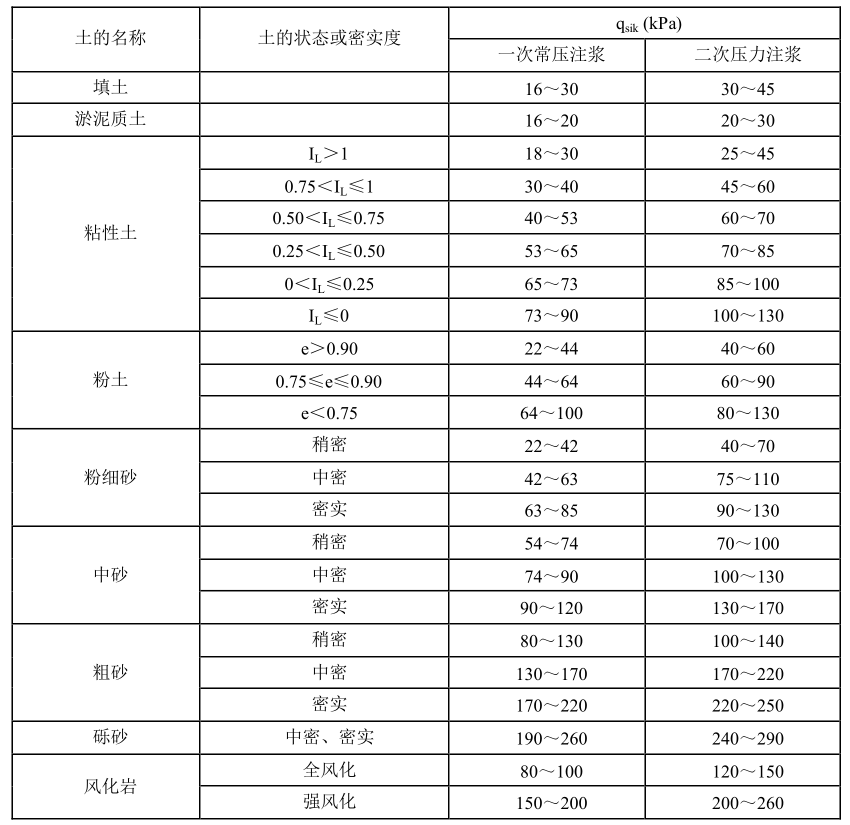
\includegraphics[width=0.8\linewidth]{figure/c8f3.png}
    \caption{锚杆的极限粘结强度标准值}
    \label{fig:c8f3}
\end{figure}

\subsection{施工安全保障措施}

(1) 基坑周围要设置安全标志警戒,提示施工人员注意安全,进入施工现场时必须佩戴安全帽。

(2) 机械和电气设备,非操作人员严禁触碰,操作人员要经过培训并持有对应的操作证件之后才可以上岗操作,在不操作的时候要关闭机械和电气的电源总开关,
有锁的设备应该及时上锁。

(3) 现场所有的特种设备都应做好登记备案,有专人维护,记录,上岗人员必须通过国家的职业技能考试,获取特种作业操作证件后才可上岗,不同班次的特种作业人员交接工作时要做好记录。

(4) 每一个用电器都要有单独的电箱控制,并且都要有锁,不得随意移动电源箱,非操作人员禁止触碰。

(5) 钢板桩插打、拔出、基坑开挖等高风险操作必须有防护员和专职的安全员在现场监督并实施防护措施才可开工。

(6) 插打桩时必须严格按照既定的方案设置基坑边线,无关人员不得逾越边线,打桩需使用专业打桩机,且操作打桩机的必须为持证上岗的打桩机操作手,操作过程中操作手必须严格遵守指令员
下发的指令,按照指令进行施工,如遇指令错误、未接到指令、或指令不清晰时严禁采取任何动作,也不得擅自开工。

(7) 基坑开挖和结构支护应该逐步交替进行,基坑应该分层开挖,开挖过程中要边挖边监测,如遇严重变形、严重偏离,路基严重沉降应立即停止开挖,立即回填,随后立即通知路政部门或设备管理单位进行养护。

(8) 在基础施工期间如遇地下不明管道和管线时,应当及时与有关部门联系,确认做好防护工作获得审批后才可继续施工。在地下管道,地下线缆,光缆附近施工时,应先征得有关部门的同意后,备齐充足的抢修材料,且拟定应急方案后才可动工。

(9) 钻孔桩施工前,应事先做好场地布置、调度和施工场所的排水降水工作。

(10) 所有施工用车辆务必保持完好状态,使用前要进行调整调试确保施工有序进行,在人多车多,施工车辆和施工人员混行的地区,应当设立临时的交通指挥人员。

(11) 电力线路周围三米范围之内禁止挖坑、挖沟、取土,堆土等,如无法避免,应当符合相关的规范和要求。



\section{施工现场安全管理措施}

\subsection{安全管理方针及目标}
\subsubsection{安全管理方针}

(1) 杜绝人身重伤、死亡责任事故,轻伤负伤率指标控制在 0.3\%;

(2) 确保安全文明标准化工地;

(3) 安全隐患排查整改率 100\%;

(4) 实现无重大设备事故、无重大火灾事故、无重大交通事故、无多人急性中毒事故;

(5) 认真贯彻中国建筑《安全生产管理手册》和《施工现场安全防护标准图册》,施工现场安全防护标准化合格率 100\%;

(6) 安全管理人员持证上岗率 100\%,特种作业管理人员持证上岗率 100\%。

\subsection{现场特种作业安全教育}

根据《安全生产法》、《建筑安全生产管理条例》、国家安全生产监督局第13号令《特种作业人员安全技术培训考核管理办法》,
特种作业人员必须经过专门培训,考试合格获得上岗证后方可进行特种作业操作。\\

(1) 电工安全教育\\

\quan{1} 作业人员,必须经专业技术培训、考试合格,方准上岗独立操作;

\quan{2} 必须穿绝缘鞋,戴好安全帽及防护手套和工作相关的防护用具。携带试电笔,不准使用无绝缘的金属工具,以免造成导线接地,短路及人身触电事故。
工作时严禁用手触摸带电设备及非绝缘部分;

\quan{3} 在施工现场检修机械设备或线路,必须在配电室拉掉相应的控制开关,并悬挂“严禁合闸”的警示牌;

\quan{4} 巡视线路或检修配电子表箱,不论线路是否停电,均视为带电,当发现故障时,应有防止跨步电压及接触电压的措施。
方可进行检修工作;

\quan{5} 对施工现场的配电箱内的漏电保护器要每周进行一次检查;\\


(2) 焊工安全教育\\

\quan{1} 焊接作业人员,必须经专业技术培训、考试合格,方准上岗独立操作。非焊工严禁进行电焊作业;

\quan{2} 操作前应检查所有工具、电焊机、电源开关及线路是否良好,金属外壳应有安全可靠的接地,进出应有完整的防护罩;

\quan{3} 操作时应穿工作服、绝缘鞋和戴电焊手套、防护面罩等安全防护用品。清除作业点周围 10 米范围内的易燃易爆物品;

\quan{4} 高处作业时,必须专人监护、系好安全带,焊工必须站在稳固的操作平台上作业,严禁将焊接电缆挂在脖颈上;

\quan{5} 焊接时二次线必须双线到位,严禁借用金属管道,金属、轨道及结构钢筋作回路地线;

\quan{6} 清除焊渣时,应佩带眼睛式面罩,防止焊渣溅入眼内或烫伤皮肤;

\quan{7} 搬运氧气瓶、乙炔气瓶时,必须装好防振圈,避免碰撞、振动;使用保管中应避免曝晒和火烤,乙炔瓶、氧气瓶及易燃物品等严禁同车运输;

\quan{8} 气瓶使用时,氧气瓶与乙炔气瓶之间不应小于 5m。 氧气瓶、乙炔瓶与切割点、明火安全距离 10 米以上;

\quan{9} 氧气瓶及压力表的部位,均不得沾染油污,不准撞击、滚动和曝晒。氧气表和乙炔表冻结时,不准用火烤或锤打,应使用热水或蒸汽解冻。 \\

(3) 铲车司机安全教育\\

\quan{1} 作业前应检查发动机的油、水应加足,各操纵杆放在空挡位置,制动灵敏可靠,灯光仪表齐全、有效方可起动;

\quan{2} 机械起动必须先鸣笛,将铲斗提升离地面 50cm 左右。行驶中可用高速档,但不得进行升降和翻转铲斗动作,作业时应使用低速档,铲斗下方严禁有人,严禁用铲斗载人;

\quan{3} 装载机不得在倾斜的场地上作业,作业区不得有障碍物及无关人员。装卸作业应在平整地面进行;

\quan{4} 向汽车内卸料时,严禁将铲斗从驾驶室顶上越过,铲斗不得碰撞车厢,严禁车厢内有人,不得用铲斗运物料;

在沟槽边卸料时,必须设专人指挥,装载机前轮应与沟槽边缘保持不少于 2m 的安全距离,并放置挡木挡掩;

\quan{5} 将大臂升起进行维护、润滑时,必须将大臂支撑稳固;

\quan{6} 作业后应将装载机开至安全地区,不得停在坑洼积水处,必须将铲斗平放在地面上,将手柄放在空挡位置,拉好手制动器。关闭门窗加锁后,方可离开。\\

(4) 挖掘机机操作员安全教育\\

\quan{1} 挖掘机司机必须经专业技术培训,考试合格取证后方可上
车独立操作。司机应熟知挖掘机的机械原理,保养规则,安全操作规程,并要按规定严格执行。严禁酒后或身体不适时进行操作;

\quan{2} 挖掘机在工作前,应向施工人员了解施工条件和任务。挖掘机进入现场后,司机应遵守施工现场的有关安全规则;

\quan{3} 挖掘机在工作前,应按照日常例行保养项目,对挖掘机进行检查、保养、调整、紧固。挖掘机在工作中,严禁进行维修、保养、紧固等工作。工作过程中若发生异响、异味、温升过高等情况,应立即停车检查;

\quan{4} 挖掘机工作时应当处于水平位置,并将走行机构刹住。若地面泥泞、松软和有沉陷危险时,应用枕木或木板垫妥;

\quan{5} 若必须在挖掘机回转半径内工作时,挖掘机必须停止回转,并将回转机构刹住后,方可进行。同时,机上机下人员要彼此照顾,密切配合,确保安全;

\quan{6} 挖掘机装载活动范围内,不得停留车辆和行人。若往汽车上卸料时,应等汽车停稳,驾驶员离开驾驶室后,方可回转铲斗,向车上卸料。挖掘机回转时,
应尽量避免铲斗从驾驶室顶部越过。卸料时,铲斗应尽量放低,但又注意不得碰撞汽车的任何部位;

\quan{7} 挖掘机回转时,应用回转离合器配合回转机构制动器平稳转动,禁止急剧回转和紧急制动;

\quan{8} 铲斗未离开地面前,不得做回转、走行等动作。铲斗满载悬空时,不得起落臂杆和行走;

\quan{9} 挖掘机不论是作业或走行时,都不得靠近架空输电线路。如必须在高低压架空线路附近工作或通过时,机械与架空线路的安全距离,必须符合规定尺寸。雷雨天气,严禁在架空高压线近旁或下面工作。
在地下电缆附近作业时,必须查清电缆的走向,并用白粉显示在地面上,并应保持1米以外的距离进行挖掘;

\quan{10} 夜间工作时,作业地区和驾驶室,应有良好的照明;

\quan{11} 挖掘机工作后,应将机械驶离工作地区,放在安全、平坦的地方。将机身转正,使内燃机朝向阳方向,铲斗落地,
并将所有操纵杆放到“空档”位置,将所有制动器刹死,关闭发动机。按照保养规程的规定,做好例行保养。关闭门窗并上锁后,方可离开;

\quan{12} 挖掘机装卸车时,应由专人指挥。装卸过程中,挖掘机在坡道上严禁回转或转向。装车时若发生危险情况,可将铲斗放下,协助制动,然后挖掘机缓缓退下。\\

(5) 起重机械操作员安全教育\\

\quan{1} 起重指挥应由技术熟练、懂得起重机械性能、经过专业培训的人员担任,持证上岗。指挥时应站在能够照顾到全面工作的地点,所发信号应事先统一,并做到准确、清楚;

\quan{2} 所有人员严禁在起重臂和吊起的重物下面停留或行走;

\quan{3} 起吊物件应使用交互捻制的钢丝绳。钢丝绳如有扭结、变形,断丝、锈蚀等异常现象,应及时降低使用标准或报废;

\quan{4} 钢丝绳中有一整股折断时、断丝数目在使用中增加很快时,该绳应立即更换。钢丝绳有明显的内部腐蚀时、钢丝绳局部外层钢丝伸长呈笼形态时,应立即报废。\\

\subsection{安全生产管理制度}
\subsubsection{安全教育制度}

\subsubsection{消防安全管理制度}

(1) 消防安全管理责任制

项目消防负责人是工地防火安全的第一责任人,负责本工地的消防安全,主要职责有:\\

\quan{1} 制定并落实消防安全责任制和防火安全管理制度,组织编制火灾的应急预案和落实防火、灭火方案以及火灾发生时应急预案的实施。

\quan{2} 对职工进行消防安全教育,组织消防知识学习,使职工懂得安全动火、用电和其他防火、灭火常识,增强职工消防意识和自防自救能力。

\quan{3} 组织火灾自救,保护火灾现场,协助火灾原因调查

\quan{4} 要掌握单位内重点部位生产储存物资的性质和灭火器材的分布情况,会使用灭火器材扑灭初起火灾。

(2) 施工现场三级动火管理制度

\quan{1} 一级动火审批制度:在禁火区域内,密闭的室内、施工现场进行动火作业,由动火部门填写动火申请表,由现场管理人员
进行检查,上报公司和上级主管部门进行核查后方可动火;

\quan{2} 在具有一定危险因素的非禁火区域进行临时焊接作业,或是在节假日期间动火,由项目负责人填写动火许可证,并附上
技术方案,经现场管理人员检查无误后上报公司安全部门,批准后方可动火;

\quan{3} 在非固定的、无危险因素的场所进行动火作业,由申请动火者填写动火申请单,经现场安全负责人审查无误后,方可动火。

(3) 消防器材与后勤管理制度

\quan{1} 在防火要害部位设置的消防器材,由该部位的消防职能人负责维修及保管。

\quan{2} 器材保管人员,应懂得消防知识,正确使用器材,工作认真负责。

\quan{3} 定期检查消防器材,发现超期、缺损的,及时向消防负责人汇报,及时更新;

\quan{4} 对进入仓库的易燃物品要按类存放,并挂设好警示牌和灭火器。

\quan{5} 经常注意季节性变化情况,气温超过 38 摄氏度时,应及时采取措施,防止易燃品自燃起火。

(4) 现场生活区防火制度

职工宿舍防火工作由宿舍长负责,其余人共同配合;

宿舍内严禁使用电热器具

宿舍内由电工接线完毕后,禁止任何人私自乱拉乱接

严禁躺在床上吸烟

职工宿舍每 50$m^2$ 布置一只灭火级别不少于 3A 的灭火器,并定期检查其可靠性。

宿舍区域安全负责人应保持高度警惕,发现危险因素及时消除隐患。

\subsubsection{特种设备安全生产管理制度}

\subsubsection{高空作业安全管理制度}

(1) 高空作业管理目标\\

安全生产目标是企业经济指标的重要组成部分,根据《安全生产法》等法律法规和行业安全管理标准,制订安全生产目标管理制度。

安全与生产、安全与效益是一个整体,当发生矛盾时,必须坚持“安全第一”的原则,遵守职业健康安全法律法规,积极为员工创造适宜的、良好的工作环境,以保护员工的身心健康和职业卫生;
为有效地消除和控制危害,需要建立本质安全的科学观念,预防是最佳的选择。需要推行科学的管理体系,建立安全标准化,实行风险预防型管理,
积极采用先进的技术、工艺和设计,树立所有意外事故和职业病都是可以预防的观念;
安全生产的保障需要人机环境的安全系统协调,从人机环境的综合治理入手,坚持不懈、持续改进,没有最好,只有更好。建立安全标准化,也建立了安全工作的长效机制。\\

(2) 高空作业安全管理规定\\

\quan{1} 审批人员赴高处作业现场,检查确认安全措施后,方可批准高处作业。 从事高处作业的单位必须进行高处作业风险分析,落实安全防护措施,方可施工;

\quan{2} 高处作业人员必须经安全教育,熟悉现场环境和施工安全要求。对患有职业禁忌症和年老体弱、疲劳过度、视力不佳及酒后人员等,不准进行高处作业;

\quan{3} 高处作业前,作业人员应检查确认安全措施落实后,方可施工,否则有权拒绝施工作业;

\quan{4} 高处作业人员要按照规定穿戴劳动保护用品,作业前要检查、作业中要正确使用防坠落用品与登高器具、设备; 

\quan{5} 高处作业应设监护人对高处作业人员进行监护,监护人应坚守岗位。高处作业前,施工单位要制订安全措施;

\quan{6} 不符合高处作业安全要求的材料、器具、设备不得使用。
高处作业所使用的工具、材料、零件等必须装入工具袋,上下时手中不得持物;不准投掷工具、材料及其他物品;易滑动、易滚动的工具、材料堆放在脚手架上时,应采取措施,防止坠落。\\

(3) 高空作业分级\\

凡在离地面两米以上进行的作业,都属于高空作业;\\

\quan{1} 作业高度在2米至5米时,称为一级高处作业;

\quan{2} 作业高度在5米以上至15米时,称为二级高处作业;

\quan{3} 作业高度在15米以上至30米时,称为三级高处作业;

\quan{4} 作业高度在30米以上时,称为特级高处作业。\\

\subsection{安全文明施工措施}
\subsubsection{文明施工管理}

项目文明施工是指保持施工场地整洁、卫生,施工组织科学,施工程序合理的一种施工活动。
实现文明施工,不仅要着重做好现场的场容管理工作,而且还要相应做好现场材料、
设备、安全、技术、保卫、消防和生活卫生等方面的管理工作。
一个工地的文明施工水平是该工地乃至所在企业各项管理工作水平的综合体现。

首先,工程项目在施工准备阶段先编制单位工程《施工组织设计》、《施工组织设计》中必须编制现场文明施工措施,并经相关部门审核、审批合格后方能组织实施。\\

文明施工应遵守以下项目:

(1) 施工现场要建立文明施工责任制,划分区域,明确管理负责人,实行挂牌制,做到现场清洁整齐;

(2) 施工现场场地平整,道路坚实畅通,有排水措施,基础、地下管道施工完后要及时回填平整,清除积土;临时水电要有专人管理,不得有长流水、长明灯;

(3) 施工现场的临时设施,包括生产、办公、生活用房、仓库、料场、临时上下水管道以及照明、动力线路,要严格按施工组织设计确定的施工平面图布置、搭设或埋设整齐;

(4) 工人操作地点和周围必须清洁整齐,做到活完脚下清,工完场地清,丢洒在楼梯、楼板上的杂物和垃圾要及时清除。严禁损坏污染成品,堵塞管道;

(5) 施工现场不准乱堆垃圾及余物。应在适当地点设置临时堆放点,并定期外运。清运垃圾及流体物品,要采取遮盖防漏措施,运送途中不得遗撒。
建筑物内清除的垃圾渣土,要通过临时搭设的竖井或利用电梯井或采取其他措施稳妥下卸,严禁从门窗口向外抛掷;

(6) 根据工程性质和所在地区的不同情况,采取必要的围护和遮挡措施,并保持外观整洁;

(7) 施工现场严禁居住家属,严禁居民、家属、小孩在施工现场穿行、玩耍;

(9) 施工现场应建立不扰民措施,针对施工特点设置防尘和防噪声设施,夜间施工必须有当地主管部门的批准。

\subsubsection{环境保护}

为加强建设工程施工现场管理,防止因建筑施工对环境的污染,依据《中华人民共和国环境保护法》等有关规定制定本措施,意在在施工过程中有效防治扬尘、
噪声、固体废物和废水等污染环境的情况。根据相关规定施工现场建立环境保护管理体系,责任落实到人,并保证有效运行。
应对施工现场防治扬尘、噪声、水污染及环境保护管理工作进行检查和对职工进行环保法规知识培训考核。按照现场常见的环境污染类别,可将环境保护规定大致分为以下三类:\\

(1) 防治大气污染:\\

\quan{1} 施工现场应采取覆盖、固化、绿化、洒水等有效措施,做到不泥泞、不扬尘。

\quan{2} 遇有四级风以上天气不得进行土方回填、转运以及其他可能产生扬尘污染的施工。  

\quan{3} 施工现场有专人负责环保工作,配备相应的洒水设备,及时洒水,减少扬尘污染。  

\quan{4} 建筑物内的施工垃圾清运必须采用封闭式容器吊运,严禁凌空抛撒。施工现场设密闭式垃圾站,施工垃圾、生活垃圾分类存放。施工垃圾清运时提前适量洒水,并按规定及时清运消纳。  

\quan{5} 土方、渣土和施工垃圾的运输,必须使用密闭式运输车辆,并与持有消纳证的运输单位签定防遗撒、扬尘、乱倒协议书。施工现场出入口处设置洗车池。  

\quan{6} 施工现场混凝土浇注使用预拌混凝土,施工现场装修阶段设置搅拌机的机棚必须封闭,并配备有效的降尘防尘装置。  

\quan{7} 拆除旧有和大临建筑时,随时洒水,减少扬尘污染。渣土要在拆除施工完成之日起三日内清运完毕,并遵守拆除工程的有关规定。  \\

(2) 防治水污染:\\

\quan{1} 搅拌机、混凝土输送泵及运输车辆清洗处设置二级沉淀池,废水不得直接排入市政污水管网,经二次沉淀后用于洒水降尘。  

\quan{2} 现场存放油料、油质脱模剂,必须对库房进行防渗漏处理,储存和使用采取防泄漏措施,防止油料泄漏,污染土壤水体。\\

(3) 防治噪声污染:\\

\quan{1} 施工现场遵照《中华人民共和国建筑施工场界噪声限值》制定降噪措施。建筑施工过程中使用的设备,可能产生噪声污染的,按有关规定向工程所在地的环保部门申报。  

\quan{2} 施工现场的电锯、电刨、搅拌机、固定式混凝土输送泵、大型空气压缩机等强噪声设备搭设封闭式机棚,并尽可能设置在远离居民区的一侧,以减少噪声污染。  

\quan{3} 因生产工艺上要求必须连续作业或者特殊需要时,确需在 22 时至次日 6 时期间进行施工的,在施工前到工程所在地建设行政主管部门提出申请,经批准后方可进行夜间施工,做好周边居民工作。并公布施工期限。  进行夜间施工作业时,应采取措施,最大限度减少施工噪声,采用低噪声震捣棒等方法。
承担夜间材料运输的车辆,进入施工现场严禁鸣笛.装卸材料应做到轻拿轻放,最大限度地减少噪声扰民。  

\quan{4} 施工现场进行噪声值监测,监测方法执行《建筑施工场界噪声测量方法》,噪声值不超过国家或地方噪声排放标准。  

\subsection{安全保障措施}
\subsubsection{基坑工程安全保障措施}

\subsubsection{钢筋工程安全保障措施}

\subsubsection{模板工程安全保障措施}

\subsubsection{混凝土工程安全保障措施}

\subsubsection{砌筑工程安全保障措施}

\subsubsection{脚手架搭拆工程安全保障措施}

\subsubsection{施工用电安全保障措施}

\subsubsection{施工机具安全保障措施}

\section{施工现场事故应急预案}
\subsection{总则}
\subsubsection{编制目的}

为了保障施工生产的正常进行,对潜在的事故作出应急准备与响应。防止施工企业施工现场的生产安全事故发生,完善应急工作机制,在工程项目发生事故状态下,迅速有序地开展事故的应急救援工作,
预防或减少可能造成的人员伤亡或者财产损失,最大限度的控制危险,认真落实“安全第一、预防为主、综合治理”的安全成产方针而制定本预案。

\subsubsection{编制依据}

(1)	《中华人民共和国安全生产法》

(2) 《特种设备事故应急预案编制导则》 GB/T 33942-2017

(3) 《生产经营单位安全生产事故应急预案编制导则》 GB/T 29639-2013

(4) 《生产安全事故应急演练指南》 AQ/T 9007-2011

(5) 建设部 《工程建设重大事故和调查程序规定》

(6) 项目相关规定以及建筑工程安全操作规程

\subsection{应急组织体系}
\subsubsection{事故应急救援组织体系与主要职责}

项目部应急指挥中心领导组下设应急指挥中心办公室,下分七个小组,分别为联络调度组、抢险救援组、医疗救助组、物资保障组、事故调查组与善后组,项目应急指挥组织机构见图 \ref{fig:c8f1}

\begin{figure}[thbp!]
    \centering
    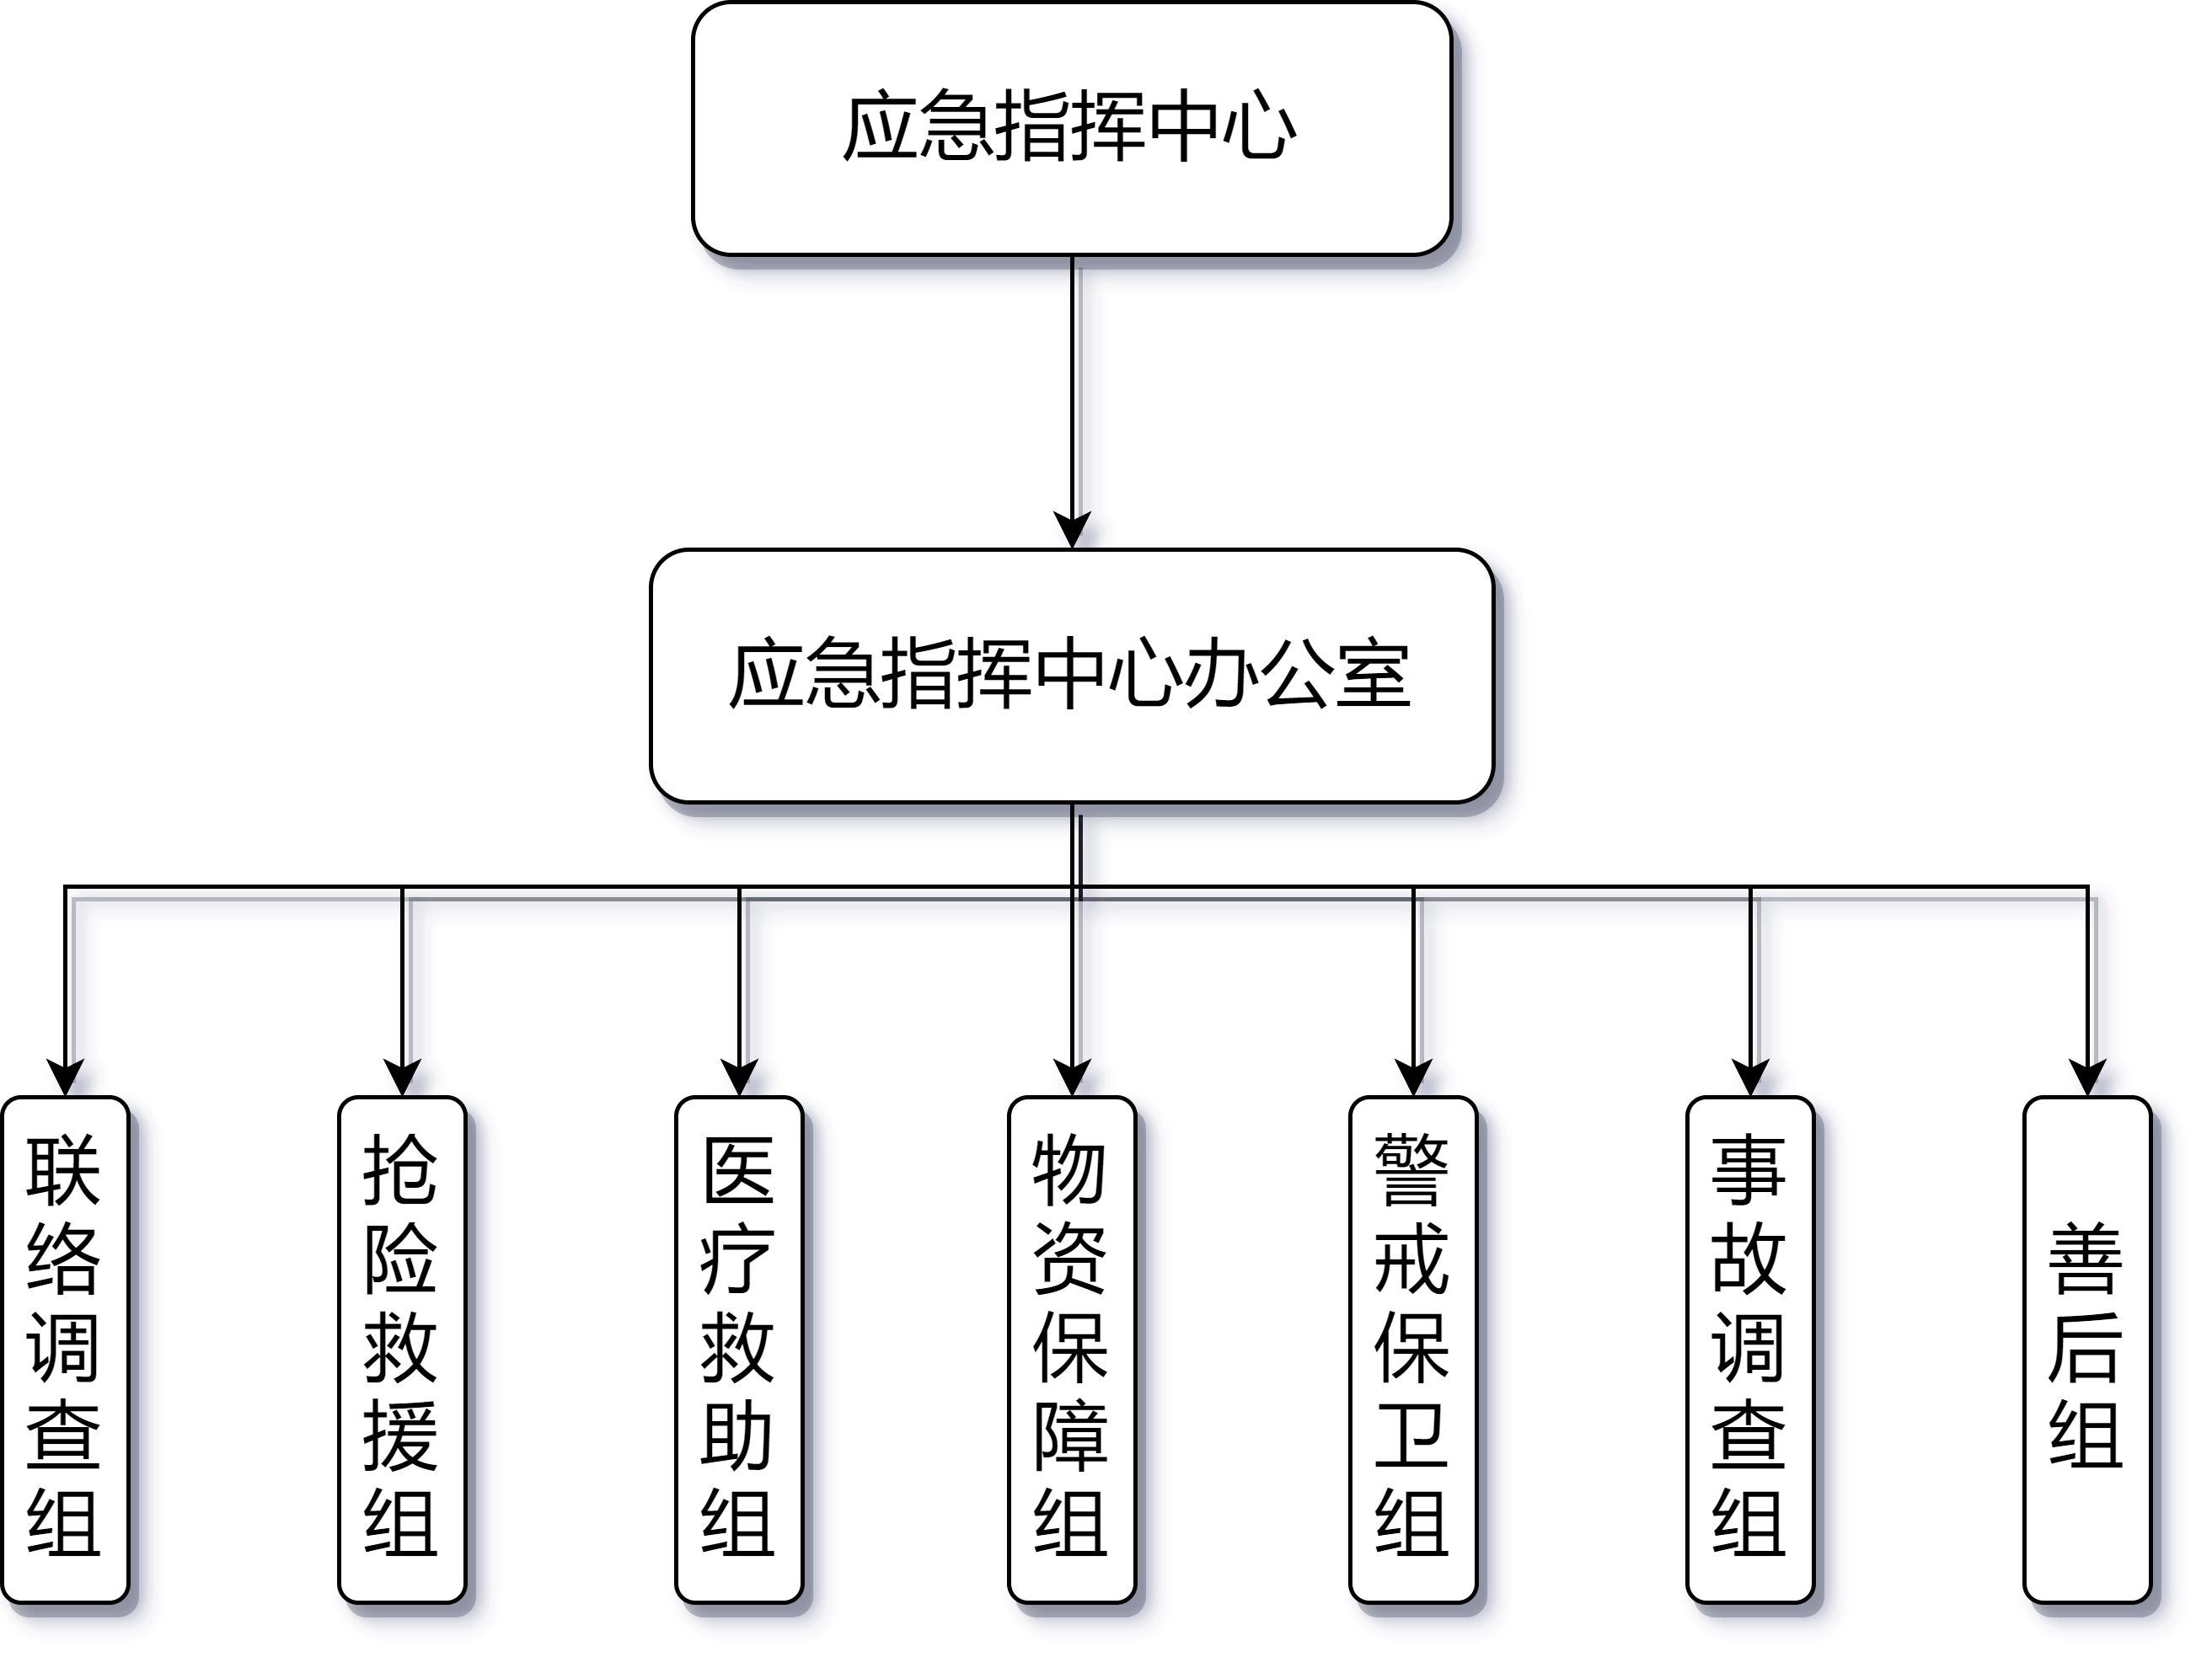
\includegraphics[width=0.8\linewidth]{figure/c8f1.png}
    \caption{项目应急指挥组织机构图}
    \label{fig:c8f1}
\end{figure}

各个组应互相紧密配合,统一领导,分工协作。处理事故时应坚持以为人本的原则,最大限度的保证人员的生命安全,控制事态发展,在确保尽可能最小化伤亡的前提下快速有效的展开救援。

\subsection{应急响应}
\subsubsection{响应分级}

根据事故严重程度、可能造成的后果以及可控性和恢复能力,项目部将应急响应级别原则上分为一级和二级两级。其中:

(1) 二级事故是发生事故险情,发生有可能影响工程正常施工或对施工有一定影响的事件时,可能导致人员受伤的或可能导致 1000 万元以下直接经济损失的事故,项目部能够自己处理的事故;

(2) 一级事故是指发生事故,发生直接导致施工中断或对施工造成极大影响的,导致有 3 人以上被困的或有人死亡或重伤的、导致 1000 万元以上直接经济损失的,项目部无法自行处理的,需要相关部门紧急救援的事故。 

\subsubsection{响应程序}

事故发生后,出事地点相关负责人立即向指挥中心报告险情,并同时启动现场处置方案,指挥中心接到报警后立刻对险情进行评估,确定响应等级并启动预案,详细的
响应流程见图 \ref{fig:c8f2}

\begin{figure}[thbp!]
    \centering
    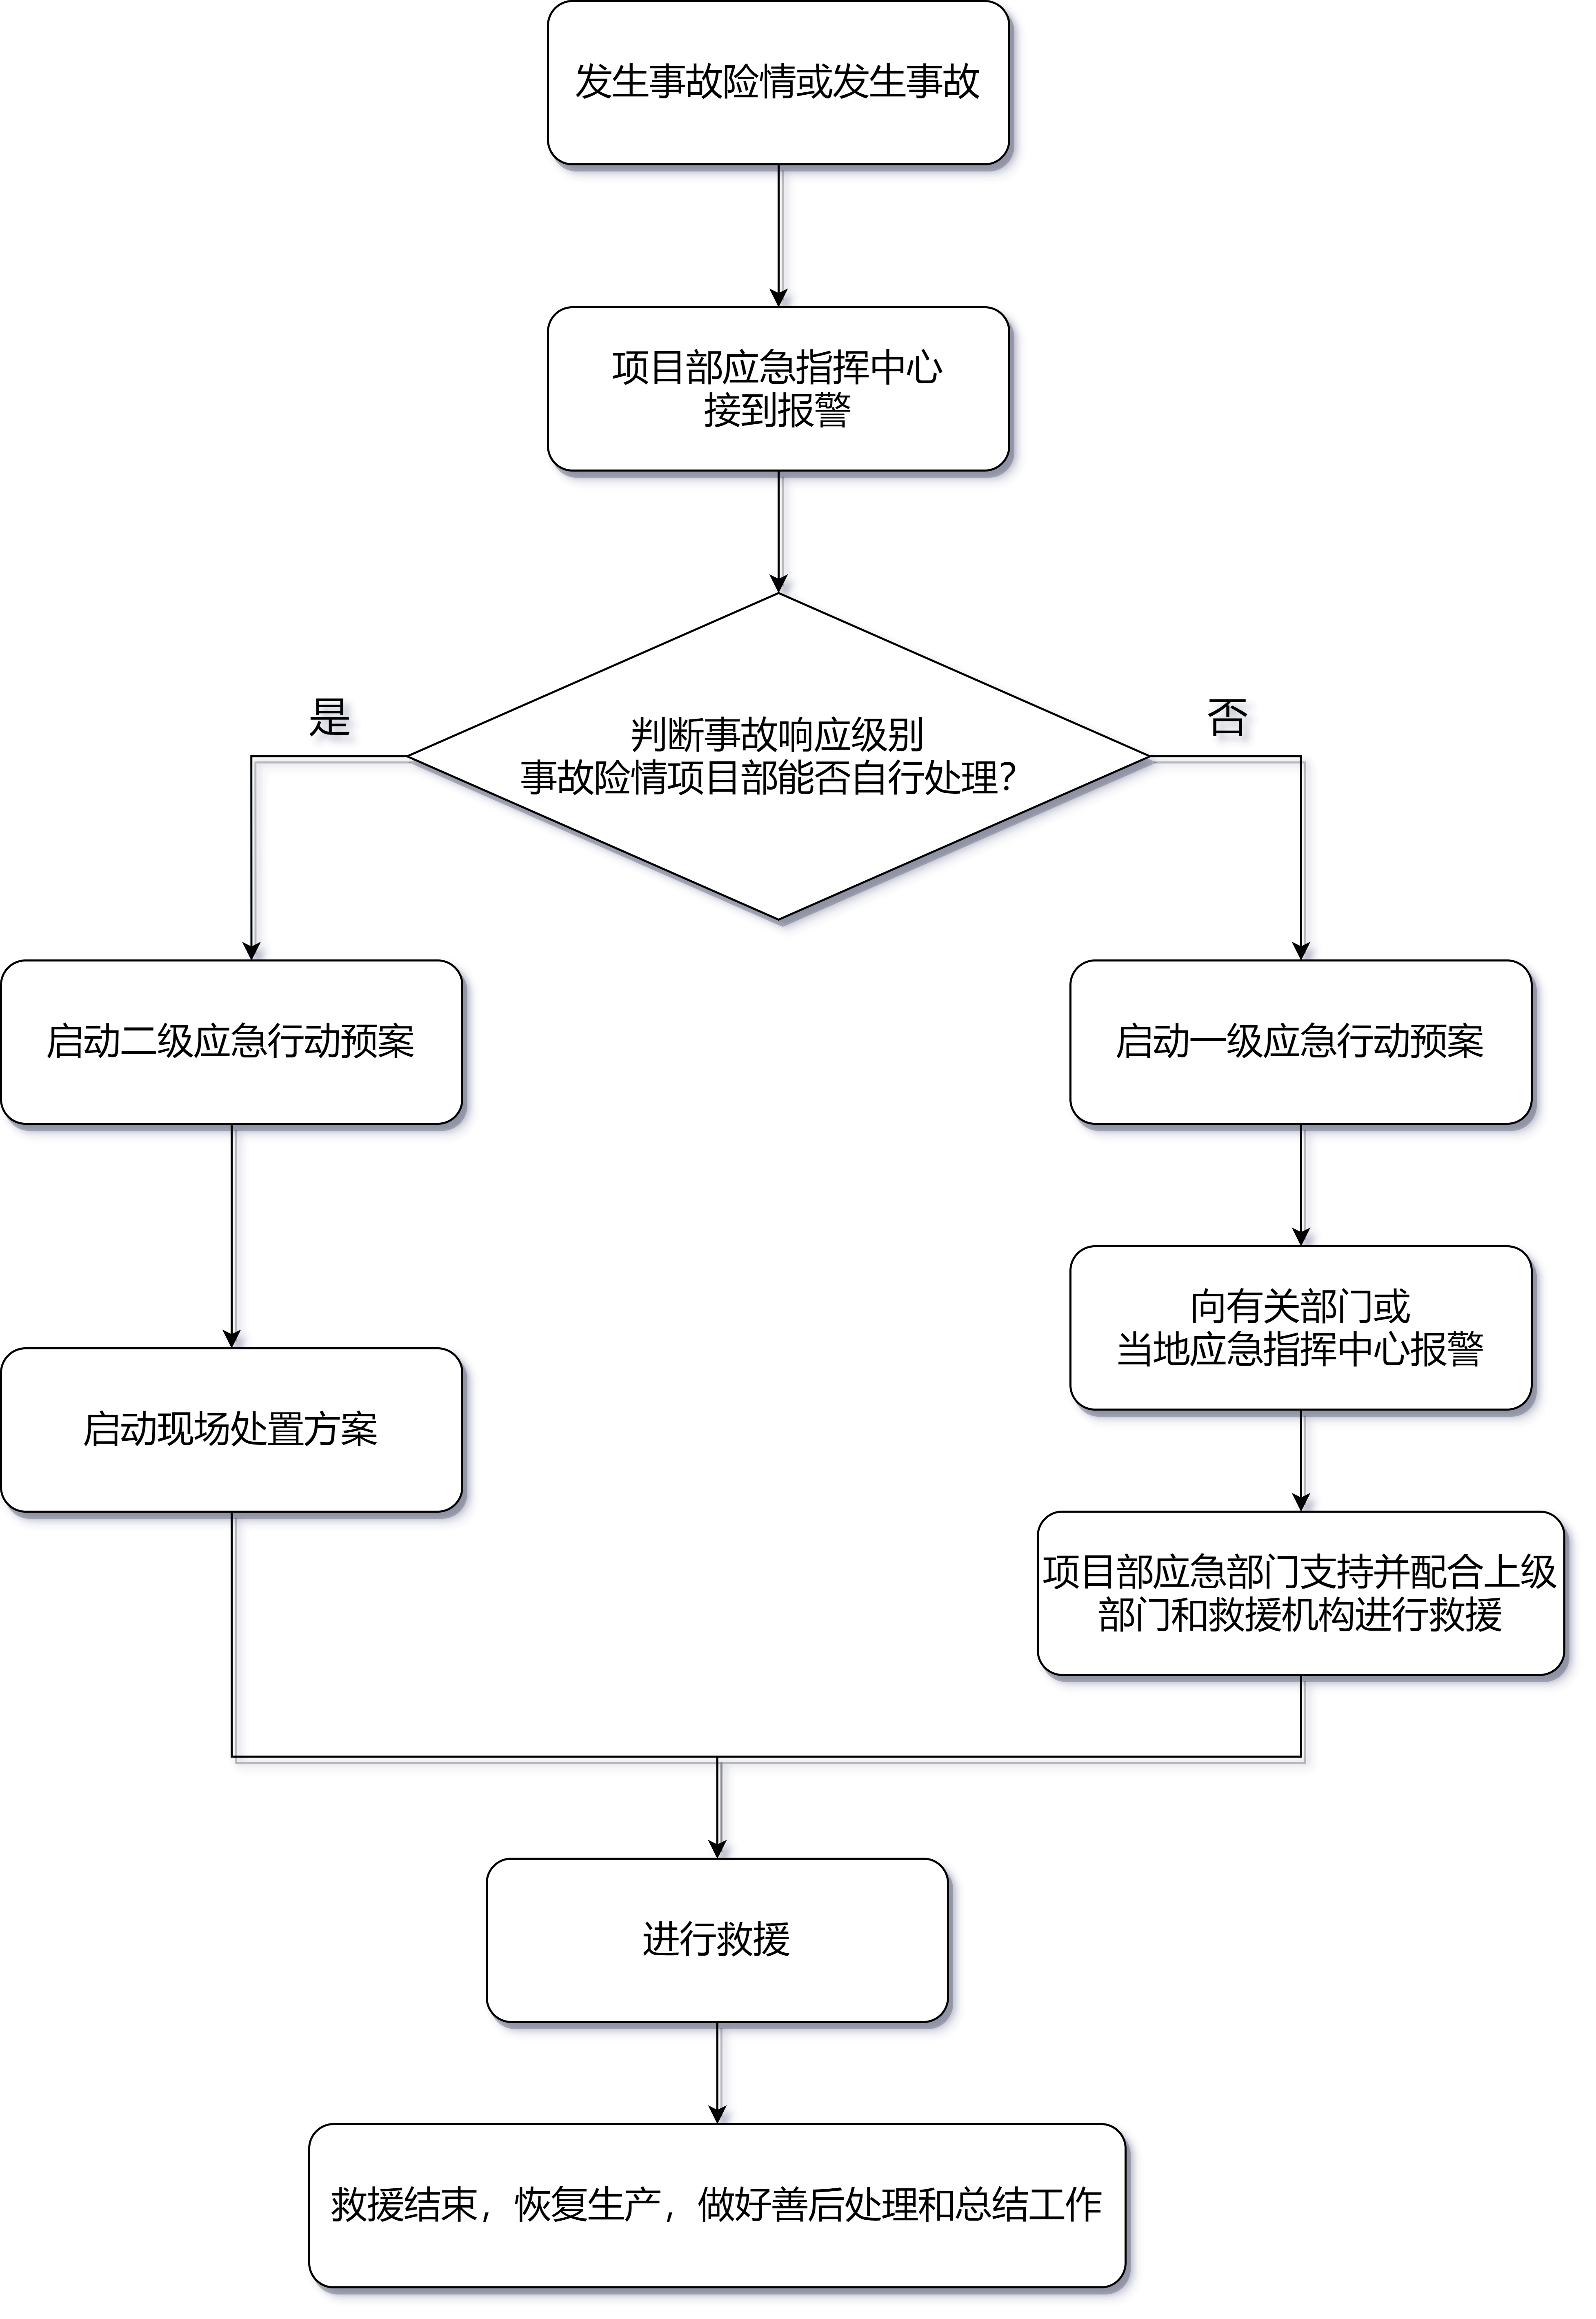
\includegraphics[width=0.8\linewidth]{figure/c8f2.png}
    \caption{项目应急响应程序流程图}
    \label{fig:c8f2}
\end{figure}

\subsection{事故应急处置}

\subsubsection{二级响应处置措施}

发生事故险情后,经指挥部确认该事故为二级事故,启动二级响应,抢险救援组率先将可能发生事故的部位接管并组织相关人员撤离,根据现场情况, 调整调集人员、设备与物质排查险情。
在响应处置过程中:

(1) 联络调度组负责维护现场秩序,将相关人员转移至安全地带,对有可能发生危险的区域进行有效的隔离;

(2) 医疗救助组负责现场的医疗抢救工作,随时待命,若发生事故则立即对受伤人员进行紧急处理,随后送往医院;

(3) 抢险救援组和物资设备保障组负责应急救援方案的主要实施,并由后勤保证组保证必要的通讯、抢救物质与设备以及自己及时到位

(4) 事故调查组在险情之后进场调查收集发生事故险情的相关资料,掌握施工险情情况,查明原因,评估事故的损失并
分清事故责任,提出防止事故发生的意见和建议,并做好书面报告。

(5) 全部疏散,安顿后停工观察,根据结果和进一步情况,明确安全等级并制定合理的复工复产计划。

\subsubsection{一级响应处置措施}

发生事故险情后,经指挥部确认该事故为一级事故,启动一级响应,抢险救援组率先将可能发生事故的部位接管并组织相关人员撤离,同时立即上报当地应急救援组织机构或地方人民政府相关机构,
应注意保护现场,已经撤离的人员不得再次靠近,等待有关部门组织专家和专业救援队伍前往现场并做好救援工作,同时,现场所有本项目部应急人员和应急小组应服从上级应急救援指挥机构的指挥。

\subsubsection{事故应急处置结束}

事故结束后,现场得以控制,次生与衍生灾害结束后,经过事故现场应急指挥机构批准后,现场应急状态结束。

应急状态结束后,又项目事故调查组负责收集事故资料,掌握事故状况,查明事故原因和评估事故影响程度和损失,查明事故责任并提出相应意见,以书面的形式汇报事故的详情,并提出防止事故再次发生的建议。

\subsection{事故后期处置}

事故处理结束后,现场应急指挥中心领导小组对现场要进行妥善的处理,包括证据的收集和现场的处理以及相关设施的重建并能尽快保证能够恢复生产,并要分析事故原因,总结经验教训,并采取预防措施。

\subsection{事故应急保障措施}
\subsubsection{应急队伍保障}

项目部应急管理中心下属的施工队每个队都应配备同等规模的应急小分队,平时项目部应加强对应急小分队的应急安全教育与培训,定期参观项目演练并亲自参与其中,做到一旦发生险情并能及时进入抢险救援状态,
能够顺利确保应急预案的有效实施。

\subsubsection{应急物资装备保障}

项目部应急指挥中心安排其下属的物资设备保障组负责项目的应急物资管理以及装备的储备及临时调配工作。

按照应急常态化的要求,物资设备保障组应当做到能够确定应急物资、设备和防护用品的数量,品类和状态,对有缺失,损坏和性能下降的物资以及耗材等应及时做好更新补充,维修和替换。

\subsubsection{其他保障}

(1) 交通运输

发生事故之后项目部应立即对现场和施工区域进行交通管制,为救援车辆和团队开辟应急特别通道,保障救援物资器材能及时准确的送达事故现场并能满足伤员的及时运出。

(2) 秩序与技术

应急响应时,又项目部警戒保卫组保障无关人员不得进入现场;同时要协助技术人员尽快倒搭现场,为救援队提供应激状态下的技术支持。

(3) 医疗与后勤

应急响应时,项目医疗救助组复制第一时间急救事故现场受伤人员,包括伤员的运出,现场对伤员的应急处置以及后续的输送伤员到正规医疗机构,直至伤员收到妥善救治;同时善后组负责后勤保障工作,协助整个
应急系统的正常运转,确保整个运转体系高效无虞。

\subsection{培训与演练}
\subsubsection{培训}

项目部应该对参加应急预案的各个部门和人员统一组织培训,目的在于发生险情时现在应急人员能够准确有效的进行应急处置,市应急救助人员具有充沛的应急救援知识和能力,培训磨合应急部门与其余部门的
协调和统一安排调度与指挥。

\subsubsection{演练}

在正式演练前,项目部应当召开演练前专项会议,协调各个部门的人员配备,并向参练人员明确其工作职责。项目部结合之前商定的元进行专项演练,对于在演练中发现的问题,应及时对预案的可行性进行整理和修改,
并杜绝相同问题在真正的应急救援中不再发生。

\subsection{火灾事故应急演练}
\subsubsection{指导思想}

通过举行火灾事故应急救援演练,事故风险较高部门和岗位的员工掌握突发火灾事故的应急救援程序、
消防器材操作使用方法和自救逃生方法,提高现场管理人员和救援人员的协调和快速应急反应能力,
从而进一步提高全体员工的自我保护意识和安全意识及自我保护能力。

\subsubsection{组织与安排}

(1) 演练领导小组\\

成员构成:配备配备总指挥一名和副总指挥一名

职责:负责演练活动筹备期间和实施过程中的领导与指挥工作。\\

(2) 演练策划组\\

成员构成:配备一名组长和三名组员

职责:负责制定演练方案以及对参与演练人员的指导和培训。\\

(3)	执行组\\

成员构成:配备一名组长和三名组员

职责:负责应急演练中与相关部门的联络、协调工作。负责情景事件要素设置及应急演练过程中的场景布置;负责调度参演人员、控制演练进程。\\

(4) 保障组\\

成员构成:配备一名组长和三名组员

职责:负责应急演练筹备及实施过程中安全保障方案的制定与执行;负责所需物资的准备,以及应急演练结束后上述物资的清理归库。\\

(5) 评估组\\

成员构成:配备一名组长和两名组员

职责:负责应急演练的评估工作,撰写应急演练评估报告,提出具有针对性的改进意见和建议。

\subsubsection{火灾应急演练过程}

安排 2 名工人在模拟火灾事故地点点燃烟雾弹,点燃烟雾弹后约 9 秒钟,一名员工随即大声呼救“着火了,请求马上救火”,现场另外一员工立即用对机向公司总指挥报告情况。

总指挥下令停止生产,全部人员立刻撤离现场,各生产部门员工在主管的带领下。从生产作业点快速撤离到预定的地点集结。随后各部门主管依次向总指挥报告人员疏散结果。
应急救援小组人员(灭火队员携带灭火器)从各方位赶到指挥中心前集合,各组长依次向总指挥报告。各救援小组人员在组长带领下奔向火灾现场展开应急救援。

6 名救护人员将 3 名伤者搀扶到保安室门口进行抢救,立即拨打 120 急救中心进行救援。

事故现场隔离现场保卫拉警戒带进行隔离,并指定进入的消防车从大门进入灭火地点,禁止其他无关车辆及人员进入。

各救援小组在组长带领下从事故现场向指挥台前集中并列队。组长向总指挥报告救援情况。

\subsubsection{演练要求}

(1) 公司全体员工应当认真学习有关消防安全知识,积极参与演练。

(2) 各救援小组由小组长组织相关人员学习救援器材的正确使用和相关救援措施,了解和掌握相关救援常识。

(3) 在演练过程中各救援小组要相互配合、协同作战,服从命令、听从指挥。

(4) )应急演练过程要力求紧凑、连贯,尽量反映真实事件下采取预警、应急处置与救援的过程。

(5) 应急演练应遵照应急预案有序进行。

\subsection{施工现场专项应急预案}
\subsubsection{高处坠落事故专项应急救援预案}

(1) 事故分析\\

高处坠落事故系以物体打击为主的多种因素导致的事故。\\

人员在施工过程有由于疏忽或失去平衡等因素发生高空坠落事故后会造成严重的人员伤亡或财产损失。\\

(2) 预防与监控\\

对作业人员要加强安全教育并做好交底工作。

高处作业时重点地区设立警示牌并避免上线同时作业

应加强对人员的安全教育,对高处作业、临边防护、吊装作业等重点项目进行安全检查,做到“早发现、早报告、早处置、低风险”\\

(3) 应急报告\\

当发生高处坠落事故时,应立即组织危险区域施工人员撤离,并报告应急指挥中心,同时指挥中心迅速评估险情,并决定是否应当启动应急预案,现场报警采取喊话的方式,向指挥中心
报告时应采用电话或对讲机。

项目应急安全中心应当使用电话向医院、公安、消防或当地的应急管理机构报告,报告的内容主要是:高处坠落事故发生的时间地点、背景、造成的经济损失、人员的伤亡状况以及需要额外救助的内容。\\

(4) 处置方式\\

当启动二级响应时,由项目部迅速启动救助方案;当启动一级响应时,应迅速撤离并报告有关部门并寻求帮助。\\

当发生高处坠落事故时,施工队应急自救小组启动机械伤害应急现场处置方案,抢险救援组迅速将遇险人员迅速撤离现场,且应当根据现场状况及时调整人员排布,设备用量,调集物资搜救被困人员

联络调度组负责维护现场秩序,将获救人员转移安全地带并有效隔离现场。

医疗救助组负责现场伤员的医疗工作,对救出的人员采取紧急医疗措施,受伤程度较轻的由医疗救助组先行急救,较重的迅速联系并送往医疗机构。

抢险救援组和物资保障组负责订正救援方案,并及时布置应急通讯、物资,并由后勤组保证所需物资和资金及时到位。

善后组负责妥善安置伤员,对在事故中罹难的职工按规定对其家属做好理赔工作。

事故调查组收集事故资料并掌握事故情况。评估事故影响程度和损失,查明主次要责任,提出复工方案与意见并形成书面报告。并由项目部应急负责人向上一级的应急救援组织机构汇报。\\

\subsubsection{机械伤害事故专项应急救援预案}

(1) 事故分析\\

机械伤害事故系以机械伤害为主的多种因素导致的事故。\\

机械在施工中,因检查维修不到位,操作违章,指挥有误等条件下,已发生碰撞,坠落等事故,造成人员伤亡和财产损失。\\

(2) 预防与监控\\

\quan{1} 项目部应制定安全管理制度,随时检查机械状态,对不符合要求的设备要及时调整,要对操作人员进行定期培训

\quan{2} 要根据现场的环境、气候或地形进行分析,对机械作业范围的高风险地区进行隔离并设立必要的警示牌

\quan{3} 机械运行中,如遇突发性的断电,偏离预定运行轨迹等故障时,应按照预设的方案及时应对,并通知施工队采取相应行动防止事故发生
有可能造成人员伤亡和财产损失时,应作出预警并向项目应急指挥中心回报并提出建议,项目预警指挥中心应做好启动应急预案的准备。\\

(3) 应急报告\\

当发生机械事故时,应立即组织危险区域施工人员撤离,并报告应急指挥中心,同时指挥中心迅速评估险情,并决定是否应当启动应急预案,现场报警采取喊话的方式,向指挥中心
报告时应采用电话或对讲机。

项目应急安全中心应当使用电话向医院、公安、消防或当地的应急管理机构报告,报告的内容主要是:机械伤害发生的时间地点、背景、造成的经济损失、人员的伤亡状况、机械的损坏程度以及需要额外救助的内容。\\

(4) 处置方式\\

当启动二级响应时,由项目部迅速启动救助方案;当启动一级响应时,应迅速撤离并报告有关部门并寻求帮助。\\

当发生一般机械伤害事故时,施工队应急自救小组启动机械伤害应急现场处置方案,抢险救援组迅速切断电源防止次生伤害并将遇险人员迅速撤离现场,且应当根据现场状况及时调整人员排布,设备用量,调集物资搜救被困人员

联络调度组负责维护现场秩序,将获救人员转移安全地带并有效隔离现场。

医疗救助组负责现场伤员的医疗工作,对救出的人员采取紧急医疗措施,受伤程度较轻的由医疗救助组先行急救,较重的迅速联系并送往医疗机构。

抢险救援组和物资保障组负责订正救援方案,并及时布置应急通讯、物资,并由后勤组保证所需物资和资金及时到位。

善后组负责妥善安置伤员,对在事故中罹难的职工按规定对其家属做好理赔工作。

事故调查组收集事故资料并掌握事故情况。评估事故影响程度和损失,查明主次要责任,提出复工方案与意见并形成书面报告。\\

当发生重大机械伤害事故时,现场负责人应立即切断所有电源设备,组织全部人员撤离危险地带,并由项目部应急负责人向上一级的应急救援组织机构汇报。

\subsubsection{火灾事故专项应急救援预案}

(1) 事故分析\\

火灾是由于动火不当而导致的事故。\\

在施工过程中火灾的隐患最大,特别是在施工的高峰期,明火作业交叉,易燃材料增多,用电负荷增大,极易引发火灾

生活区,库房等地发生火灾会造成严重的人员伤亡和经济损失,甚至造成大面积停工,设备损毁,甚至危害周边项目的正常生产生活。\\

(2) 预防与监控\\

\quan{1} 项目部应根据有关法律法规,制定完备的消防管理制度,并派专人检查制度的落实情况,消防器材的配备和维护情况,对不符合
消防安全要求的点要及时整改。

\quan{2} 要集合有关部门提供的火灾预警信息,结合当地有关自然状况,人口,交通,经济等因素进行分析评估,因地制宜的采取灾情预警和防范措施。

\quan{3} 当发现火灾苗头如烟、油、色以及气味异常时,应按照现场处置方案提前应对。并通知施工队采取相应行动防止事故发生
有可能造成人员伤亡和财产损失时,应作出预警并向项目应急指挥中心回报并提出建议,项目预警指挥中心应做好启动应急预案的准备。\\

(3) 应急报告\\

当发生火灾时,应立即组织危险区域施工人员撤离,并报告应急指挥中心,同时指挥中心迅速评估险情,并决定是否应当启动应急预案,现场报警采取喊话的方式,向指挥中心
报告时应采用电话或对讲机。

项目应急安全中心应当使用电话向医院、公安、消防或当地的应急管理机构报告,报告的内容主要是:火灾发生的时间地点、背景、造成的经济损失、人员的伤亡状况、燃烧物的种类或燃烧范围,以及需要额外救助的内容。\\

(4) 处置方式\\

当启动二级响应时,由项目部迅速启动救助方案;当启动一级响应时,应迅速撤离并报告有关部门并寻求帮助。\\

当发生轻微火灾时,施工队应急自救小组启动机械伤害应急现场处置方案,抢险救援组迅速切断电源防止次生伤害并组织项目消防队进行灭火,且应当根据现场状况及时调整人员排布,设备用量,调集物资搜救被困人员

联络调度组负责维护现场秩序,将获救人员转移安全地带并有效隔离现场。

医疗救助组负责现场伤员的医疗工作,对救出的人员采取紧急医疗措施,受伤程度较轻的由医疗救助组先行急救,较重的迅速联系并送往医疗机构。

抢险救援组和物资保障组负责订正救援方案,并及时布置应急通讯、物资,并由后勤组保证所需物资和资金及时到位。

善后组负责妥善安置伤员,对在事故中罹难的职工按规定对其家属做好理赔工作。

事故调查组收集事故资料并掌握事故情况。评估事故影响程度和损失,查明主次要责任,提出复工方案与意见并形成书面报告。\\

当发生严重火灾时,现场负责人应立即切断所有电源设备,组织全部人员撤离危险地带,并由项目部应急负责人立刻向当地消防部门和向上一级的应急救援组织机构汇报。


\section{经济技术性分析}

21 世纪是高科技时代,土木工程将会引进更多的高新技术,土木工程发展极为迅猛, 
其实践和研究已取得显著成就。而随着社会的不断发展及环境不断恶化,
人们也逐渐加强了对环境保护的重视,在追求土木工程舒适性,实用性,
美观性的同时也逐渐加强了对其环保功能的重视,因此,想要确保土木工程的长期稳定的发展,
就要合理的将可持续发展观融入到其中,有效的实现新时期土木工程的可持续发展。
在这个竞争日益激烈的市场环境下,经济技术效益是建筑企业生存的保障,
而建筑企业的经济技术效益与建筑经济技术有着必然的联系。众所周知,建筑是一大能耗行业,
所需要投入的人力、物力、财力非常大,如果建筑企业不能做好经济技术,势必就会影响到建筑企业的投入成本,
进而影响到经济技术效益。另外,成本管理作为建筑工程管理一项重要的工作,能够反映出建筑企业的施工质量,
如果企业不能做好经济技术,势必就会影响到建筑工程质量。 

\subsection{节约能源消耗}

建筑节能是近年来对建筑工程提出的一种全新的设计理念,
也是当前建筑工程领域广泛实践的新技术。土木工程在施工中需要消耗大量的能源,
已驱动机械设备运转,和施工人员的正常生活。如果不将能源消耗进行严格控制,
将对我国能源产生战略性的影响。在土木工程中提倡绿色施工的概念,
对于缓解我国能源危机,提高环境保护力度,提高人们的生活质量有重要意义。 

\subsection{提高施工水平}

传统的土木工程技术虽然已经可以实现大规模建设工程的建设任务,
但是在完成工程的同时也带来了极大的环境问题,通过提倡绿色施工技术,
在施工建设过程中对环境保护和能源消耗提出严格的限制要求,
可以促使施工单位不断改进技术,寻求更好的施工方案,促进土木工程行业的迅速发展。

\subsection{技术装备管理水平的影响}
先进的技术和装备是企业在建筑行业竞争中体现优势的主要因素,
先进的管理水平更能体现设备和技术的价值最大程度提高生产效率从而降低造价成本。
%=============  结论  ======================
\begin{center}
    \section*{\zihao{-2}  \textbf{设计总结}}
    \end{center}
\addcontentsline{toc}{section}{设计总结}

对于理工类专业来说,毕业设计是一个能够考验学生综合水平的一环,毕业设计可
以很好地培养学生的综合能力,并且将大学四年所学到的知识整合起来,可以提高对规
范的理解,对课程的认知,并且能有机的把理论和实际结合起来。除此之外毕业设计也
是一次能对专业软件和画图软件,以及排版能力的综合考量。

本设计是“河南省旅游中心项目安全施工组织设计”,通过本次的毕业设计,我能
对建筑施工的流程有了一个新的认识,对现场的安全技术和安全管理措施有了全新的理
解。建筑安全作为施工过程中看似平常的一环,实际上对项目的按时保质保量完工,人
员的生命安全,项目的经济效益等都有举足轻重的地位,可以说把控好安全的项目,无
论是施工质量还是整体成本,都会是非常优秀的一个项目。建筑作为国之基础,关乎着
社会的平稳运行和经济的发展,只有安全的做完施工,项目才可能顺利完成;只有项目
顺利完成,社会的经济水平才能得到提升,因此,安全管理在今后的现在施工中显得十
分重要。

在本设计中,首先考察了拟建项目的地理位置,分析了周边的环境影响,随后对工
程进行了危险源辨识,定性的对危险的物或因素进行了分析并提出了改进和防治措施,
然后针对重点的脚手架工程、模板工程和基坑工程定量做了专项的安全设计方案,最后
在保证安全的情况下尽可能做到文明施工。针对项目上可能出现的常见事故,还提出了
应急预案和演练过程,从而基本完备的达到了安全设计的要求。
在本次设计中,我可以说是真真正正了解到了安全工程专业日后的工作方向,将四
年所学习的课程串联了起来,真正的了解到了安全评价、土木施工、基础计算以及应急
管理等课程的知识要点,并将理论与实际结合了起来,我觉得这是一个工科大学生应该
有的技能和能力。在本次设计中,通过查阅资料,老师辅导还有同学讨论,我最终完成
了这个项目的安全组织设计,同时我也体会到了土建人的不易。本次毕业设计让我留下
了难忘的经历,我也相信我以后的工作和生活会做得更好。
%============= 参考文献 =====================
\addcontentsline{toc}{section}{参考文献}
\bibliography{bibfile}


\clearpage
\include{body/appendices}
%=============  致谢  ======================
\begin{center}
    \section*{\zihao{-2}  \textbf{致 ~~ 辞}}
    \end{center}

随着论文的结尾,也标志这我的大学四年生活正式画上了句号,我也将与这所坐落在沈城的美丽的学校即将挥手告别,在
大学四年的学习与生活之中有许许多多帮助过我的,给予我关怀的人,他们有些人是我的长辈,有些人是我的老师,有些人是我的同学,甚至有些事,有些景
也都在不同时间、以不同的方式在给我加油、给我在或是志得意满,或是人生低谷时帮助我端正心态,调整方向,在此深表感谢和感激。

大学四年来,首先要感谢的是我的父母,是他们用无私的爱、无私的关怀以及毫无保留的生活支持和经济支持不计回报的支撑着我走完大学四年的学习生活。可以说
在我十五载求学生涯之中是他们给了我最大的鼓励和支持,感谢父母对我的理解和包容,也感谢他们无私奉献的爱。对父母的恩情是无论如何也报答不完的,愿我能
在余生之内始终伴随我的父母,希望他们身体健康,平平安安。

其次要感谢的是土木学院安全教研室的全体老师,我本身算不上是聪明用功的学生,感谢这些老师们不厌其烦的教导,以及在学习生活中给予我们的关怀和爱护,在
建筑大学这个小世界里,我们真真正正感受到了来着“直系老师”们的关爱,让我们在离开家庭的保护之后还能感受到充满人文的,充满老师们独有的来自长辈的关心。
在这里也祝福土木学院安全教研室贾老师在内的全体老师们万事顺遂。

我还要感谢曾经帮助过我的学长们,是你们将懵懂无知的我从一个刚离开家门的完全不自立的孩子变成了一个懂得学会付出,懂得学会与他人合作,懂得为自己的一言一行而负责,
这里特别是要感谢我的助班谢建坤,感谢他在我刚刚步入校门时给予我兄长一般的关怀;其次要感谢我在大学生通讯社认识的部长们,虽然我未能陪大家走完大学学生工作的
最后一程,但是我会永远记住你们对我的包容和支持,你们教会我的处事之道和协作之力,一定会让我在今后的日子里受益匪浅。也希望所有帮助过和希望帮助过我的学长学姐们学业有成、前程似锦、心想事成。

大学生活是我头一次离开家中,与同学一起生活,一起居住,在这里我要感谢我的室友,在四年的日子里与我共同进退,共渡难关,虽然室友之间的生活并未一帆风顺
,并未无时不刻充满正能量,但是你们依旧是我生命中非常重要的的一部分。在未来的日子里,我将无时不刻不在怀念你们与我共同
生活这几年里的点点滴滴,更感谢你们能包容我糟糕的性格和坏习惯,祝我的室友们能早日找到自己的另一半,早日过上自己所希望的生活。

除了这些常规的感谢之外,我还要感谢那些素未谋面但是却亲如兄弟的人们,感谢我“图鉴”项目中的全体成员,感谢你们在我需要鼓励时给予我鼓励,在我需要安慰时给予我安慰。特别是
要感谢谈梦飞同学,感谢你让我更好的认识我自己,认识这个社会,感谢你让幼稚的我学着成熟,学会担当。

2020 年注定是艰难的一年,也注定是充满挑战的一年,很难想象我们这代人居然以这种方式见证了历史。我们经历了一个没有团圆的春节、一个没有毕业照的毕业季和一个没有毕业典礼的大学。但我们
没有害怕,更没有放弃,因为我们相信迷雾之后必将是阳光灿烂,黑暗之后必是满山黎明,等到疫情结束之时,就是我们这代人的胜利之日,最后我要感谢的是全社会的努力,当然也包括
感谢正在工作的你,或是感谢正在发呆的我。正是因为有了大家的齐心协力,我们才蹒跚却坚定地走完了 2020 年的上半年,在接下来的日子里,大家也要满怀希望啊!长风破浪的日子,不会太远啦!

在全篇致辞的最后,我想用一句话结束我的本科生毕业论文,也想用这一句话来勉励我今后的生活。\\

天下的所有坎坷之事终将消散,唯有爱与希望将永世长存。\\

共勉。
\addcontentsline{toc}{section}{致辞}

\end{document}
%%%%%%%%%% 结束 %%%%%%%%%%
